%%%%%%%%%%%%%%%%%%%%%%%%%%%%%%%%%%%%%%%%%%%%%%%%%%%%%%%%%%%%%%%%%%%%%%%%%%%%%%%%%%%
%%%  Filename: main.tex
%%%  ---
%%%  Template for Bachelor Thesis at DTETI UGM   		
%%%  Created using thesisdtetiugm.cls
%%%  --- 
%%%  Original Written by Canggih Puspo Wibowo
%%%  [canggihpw@gmail.com]
%%%
%%% Developed by Dr.-Ing. Yohan Fajar Sidik [DTETI FT UGM]
%%% [yohanfajarsidik@ugm.ac.id]
%%% Github repo: https://github.com/Dr-Sidik/template_thesis_latex_dteti
%%%%%%%%%%%%%%%%%%%%%%%%%%%%%%%%%%%%%%%%%%%%%%%%%%%%%%%%%%%%%%%%%%%%%%%%%%%%%%%%%%%

%% Use option "bahasa" or "english" 
%%    to change the basic language used
%% User option "bachelor", "master", or "doctoral"
%% 	  to change the degree
% \documentclass[<bachelor/master/doctoral>,<bahasa/english>]{thesisdtetiugm}
\documentclass[bachelor,bahasa]{thesisdtetiugm}
%\documentclass[bachelor,english]{thesisdtetiugm}
%======================================
% Information Input
%======================================
% Input author's name and ID number
\author{Ega Rizky Setiwan}{21/479314/TK/52861}
% Input the thesis' title
\title{Optimalisasi \textit{Knowledge Extraction} dan \textit{Knowledge Retrieval} pada RAG untuk \textit{Chatbot} Kesehatan Mental}
% Program and the head of the program
\program{Teknologi Informasi}{Ir. Agus Bejo, S.T., M.Eng., D.Eng., IPM.}{198001012015041002}
% Name of department head and NIP
\departmenthead{Hanung Adi Nugroho, Ir., S.T., M.E., Ph.D., IPM.}{197802242002121001}
\major{Konsentrasi Sistem Tenaga Listrik}
\yearsubmit{2025}
\examdate{\ldots\ldots\ldots}
% Name of thesis supervisors/promotors
\addsupervisor{Dr. Bimo Sunarfri Hantono, S.T., M.Eng.}{197701312002121003}
\addsupervisor{Dr. Guntur Dharma Putra, S.T., M.Sc.}{111199104201802102}
%\addsupervisor{<<Supervisor 3>>}{<<NIP>>}
% Name of examiners
%\addexaminer{<<Examiner 1>>}{<<NIP 1>>}
%\addexaminer{<<Examiner 2>>}{<<NIP 2>>}
%\addexaminer{<<Examiner 3>>}{<<NIP 3>>}
%\addexaminer{<<Examiner 4>>}{<<NIP 4>>}
%\addexaminer{<<Examiner 5>>}{<<NIP 5>>}
%\addexaminer{<<Examiner 6>>}{<<NIP 6>>}
%\addexaminer{<<Examiner 7>>}{<<NIP 7>>}
%\addexaminer{<<Examiner 8>>}{<<NIP 8>>}
%\addexaminer{<<Examiner 9>>}{<<NIP 9>>}

%======================================

% correct bad hyphenation here [example]
\babelhyphenation[bahasa]{
  know-led-ge meng-u-cap-kan ter-struk-tur di-ha-dap-kan meng-gu-na-kan ber-ba-gai pen-de-kat-an se-per-ti men-tal me-mi-lik-i 
  per-e-ko-no-mi-an men-ja-di ke-sen-jang-an se-ma-kin la-ya-nan fe-no-me-na me-la-por-kan ke-se-hat-an in-for-ma-si chat-bot
  me-man-faat-kan eks-ter-nal mi-sal-nya di-gu-na-kan me-ning-kat-kan me-mung-kin-kan mem-per-lu-as res-pons de-sa-in im-ple-men-ta-si
  me-nge-nai di-im-ple-men-ta-si-kan  meng-ha-sil-kan be-ru- node edge nodes edges di-u-rut-kan me-re-pre-sen-ta-si-kan
  di-ban-ding-kan en-ti-tas re-la-si be-ru-pa mem-ve-ri-fi-ka-si ke-pri-ba-di-an e-mo-si-o-nal di-la-ku-kan di-re-pre-sen-ta-si-kan
  des-krip-si ber-se-su-ai-an a-kan se-la-in neigh-bor di-ha-sil-kan me-nun-juk-kan ja-wab-an lud-low graf graph di-pa-kai vec-tor vek-tor
  correct-ness re-le-van-cy re-le-van-si naive be-ri-si-ko me-nyam-pai-kan faith-ful meng-im-ple-men-ta-si-kan me-ngor-ban-kan
  prompt-ing deep-mind di-ten-tu-kan default pe-ne-rap-an sa-sar-an di-te-mu-kan ludlow near-est des-krip-tif re-le-van re-triev-al
  mem-be-ri-kan di-te-mu-kan me-ma-kan learn-ing gemini dis-course un-der-stand-ing sum-ma-ri-za-tion me-nye-le-sai-kan de-mon-stra-si 
  bah-kan ex-trac-tion me-nya-ji-kan stig-ma such hal-lu-ci-na-tion hal-lu-ci-na-tions re-sult 
}
%% Uncomment block of code below to disable hyphenation
%\tolerance=1
%\emergencystretch=\maxdimen
%\hyphenpenalty=10000
%\hbadness=10000

\begin{document}
%======================================
% Create cover etc
%======================================

%---- COVER ----
%\printcover{sample/logougm.png}{Pendadaran/Tesis/Ringkasan Tesis*}
\printcover{sample/logougm.png}{Bachelor}
% *Choose one

%---- ENDORSEMENT PAGE ----
% Select endorsement page type. If you want to use your own PDF file,  
% 	use \printendorsementpdf, or if you want to use JPG file, use 
% 	\printendorsementjpg. Otherwise, use \printendorsement.
% 	Choose one only. Comment out unused command(s).
%
\cleardoublepage \phantomsection
\printendorsement
%\printendorsementpdf
%\printendorsementjpg{sample/scanned-endorsement.jpg}

%---- DEDICATION PAGE ----
\cleardoublepage \phantomsection
\chapterstatement{contents/statement/statement}
%\chapterstatementjpg{sample/scanned-statement.jpg}

\cleardoublepage \phantomsection
\chapterdedication{contents/dedication/dedication}

%---- STATEMENT PAGE ----
% Select statement page type. If you want to use your own JPG file,  
%	use \chapterstatementjpg{<your *.jpg file path>}. Otherwise, 
%	use \chapterstatement{contents/statement/statement}.
%	Choose one only. Comment out unused command(s).
%


%---- PREFACE PAGE ----
\cleardoublepage \phantomsection
\chapterpreface{contents/preface/preface}

%======================================
% Create Table of Contents, List of Figures, List of Tables
% <Do not change this part>
%======================================
\cleardoublepage \phantomsection
\thetoc
\onehalfspacing
\tableofcontents
\singlespacing
\cleardoublepage \phantomsection
\thelot
\listoftables
\cleardoublepage \phantomsection
\thelof
\listoffigures

%======================================

%---- NOMENCLATURE PAGE ----
\cleardoublepage \phantomsection
\chapternomenclature{contents/nomenclature/nomenclature}

%---- INTISARI PAGE----
\cleardoublepage \phantomsection
\chapterintisari{contents/abstract/intisari}

%---- ABSTRACT PAGE----
\cleardoublepage \phantomsection
\chapterabstract{contents/abstract/abstract}


%======================================



%======================================
%  MAIN TEXT
%======================================
\startmain
% You can change 
%    the filename and location of the files inputted
\cleardoublepage \phantomsection
\chapter{Pendahuluan}

\section{Latar Belakang}
Kesehatan mental merupakan komponen fundamental bagi kesejahteraan individu dan masyarakat secara keseluruhan.
Isu kesehatan mental global menunjukkan tren yang mengkhawatirkan, ditandai dengan peningkatan prevalensi berbagai gangguan mental seperti depresi, kecemasan, dan stres di berbagai negara.
Sebagai contoh, penelitian yang dilakukan oleh Institute for Health Metrics and Evaluation (IHME) memperkirakan bahwa sekitar 970 juta orang, atau 12\% dari populasi global, mengalami gangguan mental pada 2019 \cite{GBD2019MentalDisorders}.
Di Indonesia, situasinya juga tidak kalah mengkhawatirkan. Khususnya pada populasi remaja, hasil temuan penelitian Indonesia - National Adolescence Mental Health Survey (I-NAMHS) yang dirilis pada tahun 2022 menyajikan gambaran yang lebih detail.
Satu dari tiga remaja Indonesia (34,9\%), setara dengan 15,5 juta jiwa, memiliki setidaknya satu masalah kesehatan mental dalam 12 bulan terakhir.
Lebih lanjut, satu dari dua puluh remaja (5,5\%), atau sekitar 2,45 juta jiwa, terdiagnosis mengalami gangguan mental dalam periode yang sama, dengan gangguan kecemasan sebagai jenis yang paling umum ditemui \cite{INAMHS2022}.
Dampak dari gangguan kesehatan mental ini sangat luas, tidak hanya memengaruhi kualitas hidup, produktivitas, dan interaksi sosial individu, tetapi juga memberikan beban signifikan pada sistem layanan kesehatan dan perekonomian.
Oleh karena itu, investasi dalam upaya peningkatan kesehatan mental sangat krusial, karena berpotensi meningkatkan kualitas kesehatan masyarakat secara umum, yang pada gilirannya akan mendukung peningkatan fungsi sosial, produktivitas, dan pertumbuhan ekonomi.

Sayangnya, akses terhadap layanan kesehatan mental yang berkualitas masih menjadi tantangan besar.
Faktor-faktor seperti stigma sosial yang kuat, keterbatasan jumlah tenaga profesional kesehatan mental yang terdistribusi tidak merata, serta biaya layanan yang sering kali tidak terjangkau oleh sebagian besar masyarakat, menciptakan kesenjangan besar antara kebutuhan dan ketersediaan layanan.
Sebanyak 71\% dari penderita psikosis tidak mendapatkan penanganan kesehatan mental \cite{WHO2022MentalHealth}. Data I-NAMHS 2022 semakin memperjelas jurang ini:
hanya 2,6\% dari remaja dengan masalah kesehatan mental yang pernah mengakses layanan yang menyediakan dukungan atau konseling untuk masalah emosi dan perilaku dalam 12 bulan terakhir.
Lebih lanjut, secara keseluruhan, hanya satu dari lima puluh remaja (2\%) yang pernah menggunakan layanan dalam 12 bulan terakhir, dan dua pertiga dari mereka (66,5\%)
hanya pernah menggunakan layanan sebanyak satu kali. Ironisnya, ketika ditanyakan mengenai penyedia layanan yang paling banyak diakses oleh mereka yang mencari bantuan, hampir dua perlima (38,2\%)
pengasuh utama menjawab petugas sekolah, yang mengindikasikan peran penting namun mungkin belum optimal dari sistem pendidikan dalam deteksi dini dan rujukan. Fenomena ini juga diperkuat oleh temuan bahwa
hanya 4,3\% dari pengasuh utama yang menyatakan bahwa remaja mereka membutuhkan bantuan untuk masalah emosi dan perilaku, meskipun data menunjukkan 34,9\% remaja mengalami masalah kesehatan mental.
Dari pengasuh utama yang menyadari kebutuhan bantuan, lebih dari dua perlima (43,8\%) melaporkan tidak mencari bantuan karena lebih memilih untuk menangani sendiri masalah remaja tersebut atau dengan dukungan
dari keluarga dan teman-teman, yang mungkin juga mencerminkan stigma atau ketidakpercayaan terhadap layanan formal. Kondisi ini mendesak perlunya inovasi untuk memperluas jangkauan dan meningkatkan kualitas dukungan kesehatan mental.
Pandemi COVID-19 juga turut memperburuk situasi, di mana 4,6\% remaja melaporkan sering merasa lebih cemas, lebih depresi, lebih kesepian, atau lebih sulit berkonsentrasi dari biasanya selama periode tersebut \cite{INAMHS2022}.

Teknologi kecerdasan buatan atau \textit{Artificial Intelligence} (AI) telah berkembang secara masif selama beberapa dekade terakhir dan mulai menggeser perubahan aktivitas manusia.
AI mengubah proses-proses tradisional yang kaku dan membutuhkan campur tangan manusia secara intens menjadi proses modern yang luwes dan minim campur tangan manusia.
Teknologi ini sudah banyak mengintervensi kegiatan sehari-hari di berbagai sektor industri seperti \textit{online shopping}, \textit{online banking}, dan \textit{mental health care} \cite{MultiIndustryAIChatbot}.
Salah satu aplikasi teknologi AI dalam kesehatan mental yang paling banyak dikembangkan adalah \textit{chatbot} atau agen percakapan.
\textit{Chatbot} kesehatan mental menawarkan potensi solusi yang menjanjikan dengan memberikan dukungan emosional awal dan informasi psikoedukasi yang mudah diakses kapan saja dan di mana saja melalui perangkat digital.
Keunggulan tersebut diharapkan dapat membantu mengatasi beberapa hambatan penderita mental disorder dalam mencari bantuan, terutama terkait dengan stigma dan aksesibilitas geografis maupun finansial \cite{CBTWoebotTest}.
Salah satu penerapan \textit{chatbot} pada bidang kesehatan mental adalah Lintang \textit{Chatbot} yang dikembangkan oleh Health Promoting University (HPU) Universitas Gadjah Mada (UGM).
\textit{Chatbot} ini menggunakan pendekatan berbasis aturan (\textit{rule-based}) yang dirancang untuk memberikan pertolongan pertama psikologis dan informasi kesehatan mental.
Pada era modern ini, \textit{chatbot} yang populer dibagun dengan basis \textit{Large Language Model} (LLM), seperti ChatGPT, Gemini, Claude, dll.
LLM merupakan model kecerdasan buatan yang telah dilatih dengan data dalam jumlah sangat besar, memungkinkannya untuk menghasilkan respons yang sangat luwes dan alami.

Meskipun menawarkan potensi yang menjanjikan, \textit{chatbot} kesehatan mental yang ada saat ini, utamanya yang berbasis pada aturan atau model generatif sederhana, masih memiliki keterbatasan.
Sering kali respons yang diberikan terasa kaku, repetitif, dan gagal memahami nuansa dalam ekspresi emosi atau pertanyaan pengguna.
Tantangan utama terletak pada kemampuan \textit{chatbot} dalam mengakses, memproses, dan menyajikan informasi yang tidak hanya akurat dan relevan, tetapi juga kontekstual dan empatik.
Pengguna sering kali membutuhkan informasi yang sangat spesifik mengenai kondisi mereka, opsi perawatan, atau fasilitas yang tersedia.
Informasi ini sering kali tidak tersedia oleh \textit{chatbot} pada umumnya karena keterbatasan terhadap data yang selalu berubah dan berkembang setiap waktu.
Keterbatasan akses tersebut dapat membuat model generatif mengalami "halusinasi", yaitu model menciptakan informasi yang terdengar meyakinkan namun tidak faktual atau tidak bersumber dari basis pengetahuan yang valid.
Lebih lanjut, memastikan bahwa basis pengetahuan \textit{chatbot} selalu terbarui, berbasis bukti ilmiah (\textit{evidence-based}), dan bebas dari misinformasi merupakan hal yang krusial, mengingat sensitivitas isu kesehatan mental.

Untuk menjawab tantangan tersebut, salah satu pendekatan yang telah dikembangkan adalah \textit{Retrieval-Augmented Generation} (RAG) \cite{Lewis2021RAGKnowledgeIntensiveNLP}.
RAG menggabungkan kemampuan menghasilkan respons yang luwes dan alami dari LLM ini dengan informasi relevan yang diambil dari basis pengetahuan.
Pendekatan tersebut diharapkan dapat membuat \textit{chatbot} memberikan jawaban yang lebih faktual, mengurangi halusinasi, dan menyajikan informasi yang lebih spesifik dan terkini karena memiliki konteks yang relevan dengan pertanyaan.
Pada umumnya, arsitektur RAG merepresentasikan basis pengetahuannya dalam bentuk kumpulan dokumen \cite{Lewis2021RAGKnowledgeIntensiveNLP}, sejalan dengan cara manusia secara alami merepresentasikan pengetahuan melalui buku, artikel, atau jurnal ilmiah.
Kumpulan dokumen yang relevan diambil oleh sistem sebagai konteks tambahan dalam menjawab pertanyaan.

Meskipun efektif dalam mengurangi halusinasi, arsitektur RAG konvensional ini memiliki keterbatasan fundamental yang berasal dari representasi datanya yang datar (\textit{flat}).
Struktur ini menghadapi kesulitan saat sistem mencoba mengambil informasi berdasarkan hubungan antar entitas.
Sistem ini seringkali kurang memiliki \textit{ contextual awareness} yang dibutuhkan untuk menjaga koherensi di berbagai entitas dan interelasinya, sehingga respons yang dihasilkan mungkin tidak sepenuhnya menjawab pertanyaan pengguna.
Sebagai contoh, dalam domain kesehatan mental, sebuah sistem mungkin dapat mengambil potongan teks tentang "Hiperaktivitas" dan potongan lain tentang "Gangguan Mental Emosional", tetapi ia kesulitan untuk secara konsisten memanfaatkan hubungan eksplisit bahwa yang satu adalah gejala untuk yang lain karena informasi tersebut berada dalam dokumen yang terpisah.
Akibatnya, jawaban yang dihasilkan bisa jadi terfragmentasi dan gagal menyajikan jawaban yang koheren.

Untuk mengatasi limitasi tersebut, penelitian terbaru mulai mengusulkan pendekatan graph-based RAG, yang mengorganisir basis pengetahuan ke dalam sebuah struktur graf.
Dalam model ini, informasi direpresentasikan sebagai \textit{node} yang melambangkan entitas (misalnya, gangguan, gejala, obat) dan \textit{edge} yang menandai hubungan semantik di antara mereka \cite{Chen2020ReviewKnowldgeReasoningOverKnowledgeGraph}.
Sebagai contoh, "Depresi Mayor" memiliki gejala "Kehilangan Minat", "Terapi Kognitif Perilaku" digunakan untuk mengobati "Gangguan Panik".
Representasi terstruktur ini, yang dikenal sebagai \textit{Knowledge Graph} (KG), memungkinkan pencarian informasi yang lebih presisi, penarikan kesimpulan (\textit{reasoning}), dan pemahaman konteks yang lebih luas dan mendalam \cite{Chen2020ReviewKnowldgeReasoningOverKnowledgeGraph}.
Adopsi basis pengetahuan berupa KG ke dalam RAG berpotensi meningkatkan kemampuan \textit{chatbot} kesehatan mental untuk memberikan penjelasan yang kaya, jawaban yang akurat atas pertanyaan-pertanyaan spesifik, dan bahkan membantu pengguna memahami hubungan antara berbagai aspek kondisi mental mereka.

Namun, efektivitas KG dalam arsitektur RAG sangat ditentukan oleh dua proses fundamental, yaitu \textit{Knowledge Extraction} (KE) dan \textit{Knowledge Retrieval} (KR).
KE adalah proses mengidentifikasi dan mengekstrak informasi terstruktur (entitas, relasi, atribut) dari berbagai sumber data (misalnya, literatur medis, jurnal psikologi, pedoman klinis, forum diskusi terkurasi) untuk membangun atau memperkaya KG \cite{Choi2025KnowledgeGraphConstruction}.
Dalam domain kesehatan mental, proses ini dihadapkan pada tantangan seperti variasi terminologi, sinonim, polisemi, dan kebutuhan krusial akan akurasi serta validitas informasi.
Ekstraksi yang tidak optimal akan menghasilkan KG yang tidak lengkap, tidak akurat, atau bias, yang pada akhirnya akan menurunkan kualitas informasi yang dapat diakses oleh sistem RAG.

Selanjutnya, \textit{Knowledge Retrieval}, yaitu proses untuk menemukan informasi yang paling relevan dengan kueri pengguna untuk diumpankan ke model generatif dalam RAG, juga merupakan aspek krusial.
Ketika pengguna berinteraksi dengan \textit{chatbot} menggunakan bahasa alami, \textit{retriever} harus mampu menyediakan informasi dari basis data yang dimiliki agar cukup untuk menjawab pertanyaan.
Proses ini harus mampu menangani ambiguitas bahasa, memahami intensi pengguna secara akurat, dan mengambil informasi yang relevan tanpa membebani model generatif dengan informasi yang berlebihan atau tidak perlu.
Metode \textit{retrieval} yang suboptimal akan menghasilkan respons yang kurang relevan, tidak lengkap, atau bahkan menyesatkan \cite{Edge2025LocalGlobalGraphRAG}.

Meskipun potensi RAG berbasis KG untuk \textit{chatbot} kesehatan mental sangat besar, penelitian yang secara spesifik berfokus pada optimalisasi proses \textit{Knowledge Extraction} dan \textit{Knowledge Retrieval} dalam konteks ini masih relatif terbatas.
Kebanyakan penelitian lebih terfokus pada pembangunan KG secara umum atau aplikasi RAG dengan sumber data teks bebas.
Padahal, optimalisasi kedua proses ini, yang disesuaikan dengan karakteristik unik dan tuntutan domain kesehatan mental seperti kebutuhan akan akurasi tinggi, empati, dan penyampaian informasi yang mudah dicerna, sangat esensial untuk memaksimalkan efektivitas dan keamanan \textit{chatbot}.
Oleh karena itu, penelitian ini bertujuan untuk menginvestigasi dan mengembangkan metode optimalisasi untuk kedua proses tersebut, guna membangun chatbot kesehatan mental yang lebih akurat, andal, dan mampu memberikan pemahaman kontekstual yang mendalam.

\section{Rumusan Masalah}
Pemanfaatan chatbot untuk layanan kesehatan mental yang aksesibel dihadapkan pada tantangan fundamental, yaitu memastikan respons yang akurat, andal, dan berbasis bukti untuk mencegah risiko misinformasi yang berbahaya bagi pengguna.
Meskipun arsitektur canggih seperti RAG yang diperkaya KG menawarkan solusi menjanjikan, implementasinya masih dihadapkan pada kendala teknis, khususnya pada komponen \textit{Knowledge Extraction} dan \textit{Knowledge Retrieval}.
Oleh karena itu, penelitian ini difokuskan untuk menjawab permasalahan sebagai berikut.
\begin{enumerate}
	\item Belum adanya rancangan arsitektur \textit{chatbot} layanan kesehatan mental yang teruji untuk menjamin konsistensi dan akurasi respons berbasis bukti, sehingga berisiko menimbulkan misinformasi yang dapat membahayakan pengguna dalam konteks kesehatan mental yang sensitif.
	\item Adanya tantangan dalam merancang proses KE yang mampu memetakan terminologi dan hubungan kompleks dari literatur kesehatan mental ke dalam struktur KG yang koheren. Kegagalan dalam memodelkan hubungan ini secara akurat akan menghasilkan KG yang tidak mampu mendukung proses \textit{retrieval} secara mendalam, menyebabkan jawaban menjadi dangkal atau tidak lengkap.
	\item Ketidakmampuan proses KR untuk secara konsisten menemukan potongan informasi yang paling relevan dari KG sebagai respons terhadap pertanyaan pengguna, berisiko membuat arsitektur RAG mengambil basis bukti yang salah atau tidak lengkap, sehingga respons yang dihasilkan menjadi tidak akurat dalam menjawab pertanyaan spesifik pengguna.
\end{enumerate}
\section{Tujuan Penelitian}
Berdasarkan rumusan masalah yang telah dipaparkan, penelitian ini memiliki beberapa tujuan spesifik yang dirancang untuk menjawab tantangan tersebut.
Adapun tujuan dari penelitian ini adalah sebagai berikut:
\begin{enumerate}
	\item Merancang dan mengimplementasikan sebuah arsitektur \textit{chatbot} kesehatan mental yang mengintegrasikan KG dan RAG untuk menghasilkan respons berbasis bukti yang konsisten dan akurat.
	\item Mengembangkan metode \textit{Knowledge Extraction} menggunakan LLM yang mampu membangun KG dengan struktur relasi yang efektif untuk mendukung proses \textit{Knowledge Retrieval}.
	\item Merancang dan menerapkan sebuah metode KR yang mampu secara akurat dan efisien menemukan informasi paling relevan dari KG sebagai respons terhadap pertanyaan spesifik pengguna, guna meningkatkan akurasi sistem RAG.
\end{enumerate}
\section{Batasan Penelitian}
\begin{enumerate}
	\item \textbf{Objek Penelitian}: Penelitian ini akan berfokus pada metode RAG berbasis \textit{Knowledge Graph} yang mencakup
	      Metode optimalisasi \textit{Knowledge Extraction} dari sumber data tekstual kesehatan mental,
	      struktur, kualitas, dan pemanfaatan KG kesehatan mental sebagai basis bukti,
	      algoritma dan strategi optimalisasi \textit{Knowledge Retrieval} dari KG untuk mendukung sistem RAG, dan
	      kualitas dan efektivitas respons berbasis bukti yang dihasilkan oleh prototipe \textit{chatbot} kesehatan mental yang dikembangkan.
	\item \textbf{Metode Penelitian}: Penelitian ini akan menggunakan pendekatan metode eksperimen dan kuantitatif.
	      Pada tahap pengembangan akan menggunakan pendekatan desain dan rekayasa sistem (\textit{design and engineering}) untuk merancang, membangun, dan mengimplementasikan metode KE dan KR pada KG.
	      Ini melibatkan studi literatur, perancangan algoritma, implementasi perangkat lunak, dan pengujian iteratif.
	      Selanjutnya evaluasi performa komponen sistem dilakukan secara kuantitatif.
	      Performa komponen \textit{retriever} dan jawaban akhir akan dibandingkan dengan \textit{golden standard}.
	\item \textbf{Waktu dan Tempat Penelitian}: Penelitian ini akan dilakukan selama periode enam bulan, dimulai pada bulan Februari 2025 hingga Juli 2025. Tempat penelitian adalah di Gedung DTETI FT UGM, dengan menggunakan VS Code untuk pengembangan dan pengujian model.
	\item	\textbf{Populasi dan Sampel}: Populasi dalam penelitian ini adalah seluruh korpus data teks yang relevan dengan domain kesehatan mental, seperti artikel ilmiah dan buku teks.
	      Sampel data dipilih dari populasi tersebut yang berupa buku dan artikel ilmiah yang tersedia pada \textit{website} \href{https://ugm.ac.id/}{UGM}, \href{https://cpmh.psikologi.ugm.ac.id/}{CPMH}, \href{https://hpu.ugm.ac.id}{HPU UGM}, dan \href{https://repository.kemkes.go.id/}{Kementerian Kesehatan}.
	\item	\textbf{Variabel}: Penelitian ini menggunakan variabel bebas berupa metode KE dan KR yang diterapkan.
	      Variabel terikat adalah performa \textit{chatbot} yang berupa kualitas respons yang dinilai berdasarkan metrik tertentu.
	\item	\textbf{Hipotesis}: Hipotesis yang diusulkan dalam penelitian ini adalah \textit{chatbot} kesehatan mental yang menggunakan RAG berbasis KG dengan optimalisasi pada KE dan KR menunjukkan peningkatan performa dibandingkan dengan \textit{chatbot} yang menggunakan pendekatan RAG standar atau tanpa KG.
	\item	\textbf{Keterbatasan Penelitian}: Penelitian ini memiliki keterbatasan pada \textit{dataset} yang digunakan sebagai basis pengetahuan dalam sistem RAG.
	      Akurasi dan kelengkapan data bergantung pada \textit{dataset} yang mungkin belum mencakup semua aspek permasalahan kesehatan mental.
	      Penelitian ini tidak mengevaluasi dampak klinis \textit{chatbot} pada kondisi psikologis pengguna melainkan hanya mengevaluasi hasil respons \textit{chatbot} dengan metrik yang tersedia.
\end{enumerate}

\section{Manfaat Penelitian}
Penelitian ini diharapkan memberikan kontribusi pada pengembangan arsitektur \textit{chatbot} yang lebih andal dan terpercaya, khususnya dalam domain yang memerlukan informasi berbasis bukti seperti layanan kesehatan mental.
Selain itu, penelitian ini juga diharapkan memberikan wawasan mengenai efektivitas arsitektur \textit{chatbot} menggunakan RAG berbasis \textit{Knowledge Graph} dalam memberikan respons yang akurat.
Dari sisi praktis, \textit{chatbot} ini dapat diimplementasikan dan memberikan dampak positif dengan membantu pengguna dalam membuat keputusan terkait dengan kesejahteraan mental mereka, dengan tetap menekankan pentingnya konsultasi profesional untuk diagnosis dan perawatan.
\section{Sistematika Penulisan}
Sistematika penulisan berisi hal yang akan dibahas dalam penelitian ini yang akan disusun menjadi 5 bab, sebagai berikut.

\begin{enumerate}
	\item \textbf{Bab I Pendahuluan} menjelaskan hal yang melatarbelakangi adanya penelitian ini, rumusan masalah yang akan coba dicari solusinya, tujuan yang ingin dicapai, serta manfaat bagi pihak-pihak terkait.
	\item \textbf{Bab II Tinjauan Pustaka dan Dasar Teori} berisi ulasan literatur penelitian yang sudah pernah dilakukan sebelumnya mengenai topik-topik yang relevan dengan pengembangan chatbot.
	      Bab ini akan menguraikan beberapa metode yang pernah dilakukan untuk meningkatkan performa \textit{chatbot} pada aplikasi tertentu, khususnya pada bidang layanan kesehatan mental.
	      Setiap metode tersebut akan diulas potensinya untuk pengembangan lebih lanjut, peningkatan yang telah dicapai, dan tantangan yang mungkin dihadapi.
	      Selain itu, bab ini juga akan disertai dengan penjelasan mengenai teori-teori yang berkaitan dengan pengembangan \textit{chatbot}, arsitektur RAG, dan penggunaan \textit{Knowledge Graph}.
	\item \textbf{Bab III Metode Penelitian} membahas langkah-langkah detail yang akan ditempuh dalam penelitian, seperti mulai dari identifikasi masalah, studi literatur, proses pengumpulan data, perancangan dan pengembangan model, hingga metode evaluasi dan analisis hasil.
	      Bab ini juga akan menjelaskan metode penelitian eksperimen dan kuantitatif yang akan dilakukan dalam penelitian ini.
	\item \textbf{Bab IV Hasil dan Pembahasan} menyajikan hasil dari implementasi dan pengujian model \textit{chatbot} yang telah dikembangkan.
	      Pada bab ini akan membahas mengenai kualitas respons dari \textit{chatbot} yang mengimplementasikan arsitektur RAG berbasis \textit{Knowledge Graph} dan dibandingkan dengan yang tidak menggunakan arsitektur tersebut.
	      Hasil temuan tersebut akan dianalisis secara mendalam dan dibandingkan dengan hipotesis serta penelitian sebelumnya.
	\item \textbf{Bab V Kesimpulan dan Saran}  berisi kesimpulan yang ditarik dari keseluruhan hasil penelitian dan pembahasan.
	      Bagian ini akan memberikan gambaran mengenai kontribusi penelitian ini dalam pengembangan teknologi \textit{chatbot} pada layanan kesehatan mental.
	      Selain itu, akan disampaikan pula saran-saran untuk pengembangan lebih lanjut dari sistem yang dibangun atau untuk penelitian terkait di masa mendatang.
\end{enumerate}
\cleardoublepage \phantomsection
\chapter{Tinjauan Pustaka dan Dasar Teori}

\section{Tinjauan Pustaka}
\subsection{\textit{Chatbot} dengan Sistem Berbasis Aturan (\textit{Rule-Based System})}
Sistem berbasis aturan (\textit{rule-based system}) merupakan salah satu pendekatan yang paling awal dalam pengembangan \textit{chatbot}.
Dalam sistem ini, alur percakapan, pertanyaan yang dapat dikenali, serta respons yang diberikan telah ditentukan sebelumnya melalui serangkaian aturan eksplisit.
Aturan-aturan tersebut umumnya dirancang secara manual oleh ahli di bidang tertentu.
Sebagai contoh, dalam konteks kesehatan mental, perancang aturan bisa berupa psikiater, psikolog, atau peneliti di bidang kesehatan.
Implementasi dari aturan-aturan tersebut dapat berbentuk struktur kondisional seperti \textit{if-then-else} yang digunakan untuk mengatur jalannya percakapan.
Karena aturan-aturan ini tertulis secara eksplisit, pengembang memiliki kendali penuh terhadap arah percakapan dan jawaban yang diberikan oleh \textit{chatbot}.
Hal ini memungkinkan \textit{chatbot} merespons pertanyaan pengguna secara konsisten dan sesuai dengan skenario yang telah ditentukan.

Salah satu pionir \textit{chatbot} berbasis aturan adalah ELIZA, yang dikembangkan oleh Joseph Weizenbaum di Massachusetts Institute of Technology (MIT) pada tahun 1966.
ELIZA dirancang untuk menyimulasikan percakapan antara pasien dan psikoterapis aliran Rogerian, dengan memanfaatkan teknik \textit{pattern matching} (pencocokan pola) dan \textit{substitution} (penggantian kata).
Sistem ini mencocokkan masukan pengguna dengan pola-pola tertentu yang telah didefinisikan dalam skrip. Pola-pola tersebut biasanya mengandung \textit{wildcard} seperti simbol * (\textit{asterisk}), yang memungkinkan sistem menangkap frasa dari masukan pengguna dan menyusunnya kembali dalam bentuk respons yang sesuai \cite{Weizenbaum1966ELIZA}.

Di Indonesia, salah satu contoh implementasi \textit{chatbot} berbasis aturan adalah Lintang, sebuah \textit{chatbot} yang dikembangkan oleh HPU UGM.
\textit{Chatbot} ini dirancang untuk melakukan skrining awal masalah kesehatan mental dan memberikan pertolongan pertama psikologis.
Lintang dilengkapi dengan berbagai fitur utama seperti psikoedukasi yang menyediakan informasi penting mengenai kesehatan mental, termasuk berbagai gangguan, gejala, dan strategi bantuan diri.
Tips kesehatan mental yang memberikan saran untuk merawat dan meningkatkan kesehatan mental, seperti teknik relaksasi, manajemen stres, dan promosi kesejahteraan emosional.
Fitur swaperiksa yang memungkinkan pengguna melakukan evaluasi awal kondisi kesehatan mental dengan menjawab sejumlah pertanyaan.
Terakhir, direktori layanan yang menyajikan informasi mengenai sumber daya dan layanan kesehatan mental yang tersedia di lingkungan fakultas maupun universitas \cite{Lintang}.

Sistem berbasis aturan menawarkan keunggulan dari segi kontrol penuh akan alur percakapan dan respons yang dihasilkan.
Hal tersebut menjadikannya cocok diimplementasikan pada aplikasi yang membutuhkan struktur dialog ketat dan dapat diprediksi seperti pada ELIZA dan Lintang.
Namun, pendekatan ini memiliki tantangan pada skalabilitas dan fleksibilitas.
Sistem akan menjadi sangat kompleks dan sulit untuk dipelihara seiring bertambahnya variasi masukan pengguna karena semua aturan harus di bangun secara manual.
Selain itu, \textit{chatbot} cenderung tidak mampu untuk memahami dan menangani percakapan yang sifatnya terbuka atau tidak terduga.


\subsection{\textit{Chatbot} dengan \textit{Fine-Tuning Large Language Model}}
\textit{Chatbot} mengalami perkembangan yang signifikan seiring dengan kemajuan teknik \textit{Natural Language Processing} (NLP), khususnya dengan adanya \textit{Large Language Model} (LLM) seperti GPT, Gemini, Qwen, Llama, dll.
LLM memungkinkan terjadinya interaksi percakapan yang luwes antara manusia dan mesin.
\textit{Language model} ini dilatih menggunakan sumber data yang masif, sehingga mampu memahami dan menghasilkan teks dengan konteks yang luas dan alami.
Namun, LLM mengalami kesulitan saat diimplementasikan pada kasus yang spesifik, seperti menjadi \textit{chatbot} kesehatan mental untuk suatu instansi.
Jawaban yang diberikan LLM sering kali bermasalah, seperti terlalu umum, berhalusinasi, dan tidak faktual.
Untuk itu, banyak dikembangkan metode seperti \textit{fine-tuning} untuk menutupi celah tersebut.

\textit{Fine-tuning} banyak dilakukan untuk melatih suatu \textit{language model} sehingga dapat sangat mahir pada domain tertentu.
Sebuah penelitian oleh Yu pada tahun 2024 mencoba mengeksplorasi metode untuk meningkatkan performa \textit{chatbot} untuk dukungan kesehatan mental.
Penelitian tersebut menunjukkan adanya peningkatan performa umpan balik \textit{chatbot} setelah dilakukan \textit{fine-tuning}.
Hasil evaluasi menunjukkan penggunaan \textit{fine-tuning} pada LLM DialoGPT (sekitar 1,5 B parameter) memiliki kualitas percakapan yang lebih relevan dan akurat, dengan skor BLEU mencapai 0,32 yang lebih tinggi dibandingkan GPT 3 (sekitar 175 B parameter) tanpa \textit{fine-tuning} yang hanya mencapai 0,13 \cite{yu2024FineTuneOnMentalHealthChatbotExperimental}.
Dari hasil tersebut terlihat potensi besar \textit{fine-tuning} dalam meningkatkan performa LLM untuk kasus tertentu.

\textit{Fine-tuning} terbukti secara signifikan meningkatkan performa \textit{language model} dalam menghasilkan umpan balik yang lebih relevan dan kontekstual, sebuah kapabilitas yang krusial khususnya dalam aplikasi layanan kesehatan mental.
Tingkat keberhasilan peningkatan ini sangat ditentukan oleh kualitas dan relevansi data yang digunakan selama proses \textit{fine-tuning}.
Model yang dihasilkan secara inheren akan mencerminkan karakteristik data pelatihannya.
Meskipun demikian, implementasi \textit{fine-tuning} menghadapi tantangan, terutama ketika berhadapan dengan basis pengetahuan yang sering berubah atau dinamis.
Kebutuhan untuk melakukan \textit{fine-tuning} ulang secara berkala demi menjaga model tetap \textit{up-to-date} memerlukan alokasi sumber daya komputasi yang besar, baik dari segi waktu, maupun daya pemrosesan.


\subsection{Penggunaan \textit{Prompt Engineering} pada \textit{Large Language Model} (LLM)}
\textit{Large Language Model}, yang dilatih pada korpus data tekstual masif, menunjukkan kinerja yang luar biasa dalam berbagai tugas pemahaman dan \textit{text generation}, bahkan sering melampaui manusia pada tugas pengetahuan umum.
LLM beroperasi dengan mengkodekan input teks ke dalam suatu ruang vektor berdimensi tinggi yang merepresentasikan hubungan semantik antar kata dan frasa.
Representasi vektor tersebut yang kemudian menjadi dasar bagi model untuk menghasilkan output teks yang relevan, koheren, dan sesuai dengan konteks yang diminta.
Kualitas respons dapat dipengaruhi oleh berbagai faktor, termasuk \textit{prompt} yang diberikan, \textit{hyperparameter} model, dan keragaman data pelatihan \cite{Chen2025UnleashingPotentialPromptEngineering}.
Dalam aplikasinya \textit{prompt} merupakan input dari model, mengubah \textit{prompt} dapat menghasilkan hasil yang berbeda secara signifikan \cite{Kaddour2023ChallengesApplicationsLLM}.
Untuk itu, \textit{prompt engineering}, pendekatan sistematis dalam merancang \textit{prompt}, memiliki peran krusial dalam memaksimalkan kinerja LLM.


Publikasi \textit{"Language Models are Few-Shot Learners"} oleh Brown et al. 2020 memberikan gambaran bahwa LLM seperti GPT-3 dapat dimaksimalkan dalam menyelesaikan tugas NLP menggunakan metode \textit{in-context learning} \cite{LLMisFewShot2020}.
\textit{In-context learning} merupakan paradigma dalam \textit{Natural Language Understanding} (NLU), di mana demonstrasi tugas ditambahkan ke dalam input \textit{prompt} sehingga \textit{pre-trained model} dapat menangani tugas tersebut tanpa memodifikasi parameter di dalamnya \cite{Dong2024SurveyInContextLearning}.
Penelitian ini membuka pengetahuan baru bahwa untuk memaksimalkan sebuah model dalam suatu tugas khusus dapat dilakukan tanpa memodifikasi bobot model (\textit{fine-tuning}).
Model yang cukup besar dapat "belajar" untuk melakukan tugas hanya dari beberapa contoh yang diberikan dalam \textit{prompt} itu sendiri, tanpa memodifikasi model itu sendiri \cite{LLMisFewShot2020}.
Brown et al. mengeksplorasi tiga variasi \textit{in-context learning} yang dibedakan berdasarkan banyaknya contoh demonstrasi yang diberikan dalam \textit{prompt}, sebagai berikut.

\begin{enumerate}
	\item \textbf{\textit{Few-Shot Prompting}} \\
	      Model diberikan beberapa contoh demonstrasi tugas pada saat inferensi. Suatu contoh biasanya memiliki konteks dan penyelesaian yang diinginkan.
	      \textit{Few-shot} bekerja dengan memberikan $K$ buah contoh konteks dan penyelesaiannya, diikuti oleh input target yang harus diselesaikan oleh model.
	      $K$ biasanya berentang antara 10 s.d 100 bergantung dengan \textit{context window} model \cite{LLMisFewShot2020}.
	\item \textbf{\textit{One-Shot Prompting}} \\
	      Model diberikan 1 contoh demonstrasi ($K=1$) beserta deskripsi dari tugas yang akan dikerjakan dalam bahasa alami.
	      Contoh demonstrasi tersebut berfungsi sebagai panduan bagi model untuk memahami input sehingga menghasilkan output yang diharapkan \cite{LLMisFewShot2020}.
	\item \textbf{\textit{Zero-Shot Prompting}} \\
	      Model diminta untuk melakukan tugas hanya berdasarkan deskripsi bahasa alami dari tugas tersebut tanpa diberikan contoh demonstrasi ($K = 0$).
	      Sebagai contoh untuk tugas terjemah bahasa \textit{"Terjemahkan kalimat bahasa Inggris berikut ke Bahasa Indonesia"} \cite{LLMisFewShot2020}.
\end{enumerate}

Tiga variasi \textit{prompt} tersebut kemudian diuji pada model GPT-3 untuk menyelesaikan beberapa tugas khusus.
Pada tugas \textit{cloze and completion}, GPT-3 dengan 3 metode \textit{prompt} secara signifikan melampaui SOTA (\textit{State of the Art}) pada \textit{dataset}
LAMBADA (\textit{LAnguage Modeling Broadened to Account for Discourse Aspects}) dengan peningkatan akurasi dari 68,0 (SOTA Turing-NLG) menjadi 86,4 (\textit{few-shot}), 72,5 (\textit{one-shot}), dan 76,2 (\textit{zero-shot}).
Pada kasus uji lain, penggunaan \textit{prompt engineering} juga menunjukkan performa yang mendekati \textit{state-of-the-art} sistem yang sudah dilakukan \textit{fine-tuning}.
Hasil tersebut menunjukkan bahwa metode \textit{few-shot} memberikan peningkatan performa paling tinggi, disusul dengan \textit{one-shot} dan \textit{zero-shot}.

Sebuah penelitian oleh Islam et al. (2025) yang berjudul \textit{"LLM-based Prompt Ensemble for Reliable Medical Entity Recognition from EHRs"} menunjukkan bahwa teknik \textit{prompting} mempengaruhi output model secara signifikan.
Penelitian ini secara khusus menyelidiki teknik \textit{entity extraction} pada bidang medis berbasis \textit{prompt} menggunakan LLM GPT-4o dan DeepSeek-R1.
Teknik \textit{prompting} seperti \textit{zero-shot}, \textit{few-shot}, dan \textit{ensemble} pada GPT-4o dan DeepSeek-R1 dievaluasi untuk mencari tahu efektivitas dari teknik dan LLM tersebut dalam tugas \textit{medical entity recognition}.
Khusus pada \textit{few-shot}, contoh demonstrasi yang ditambahkan pada \textit{prompt} dibagi menjadi 3 perlakuan, yaitu \textit{few-shot 1} berupa 1 sampel dokumen berlabel, \textit{few-shot 2} berupa 100 kalimat berlabel yang diambil dari 5 dokumen, dan \textit{few-shot 3} berupa sejumlah 5.355 contoh entitas.
Untuk teknik \textit{ensemble} melibatkan 4 jenis \textit{prompting} sebelumnya yang kemudian dilakukan semacam voting untuk menentukan hasilnya.
Dari hasil pengujian diperoleh teknik \textit{few-shot 3} memperoleh akurasi paling tinggi sebesar 0,65 pada ekstraksi entitas disusul dengan \textit{few-shot 2}, \textit{few-shot 1}, \textit{zero-shot}, dan \textit{ensemble} sebesar 0,59, 0,56, 0,37, dan 0,37.
Namun, pada pengujian klasifikasi entitas, teknik \textit{few-shot 3} justru mendapat nilai F1 paling rendah sebesar 0,86 yang berkebalikan dengan teknik \textit{ensemble} yang memiliki nilai F1 paling tinggi sebesar 0,95 dan \textit{few-shot 2} dan \textit{few-shot 1} sebesar 0,94.
Hasil tersebut membuktikan bahwa \textit{prompt engineering} meningkatkan performa LLM dalam tugas tertentu, khususnya ekstraksi entitas.

\subsection{Implementasi Arsitektur \textit{Retrieval-Augmented Generation} pada \textit{Chatbot}}
\textit{Retrieval-Augmented Generation} (RAG) merupakan metode yang ada seiring dengan perkembangan LLM yang pesat.
LLM standar sangat mahir dalam memberikan umpan balik yang bersifat umum.
Namun, pada kasus khusus, LLM mengalami kesulitan dalam memberikan respons dan cenderung menghasilkan informasi yang tidak akurat dan relevan (halusinasi).
Informasi yang dimiliki oleh LLM hanya terbatas oleh data yang digunakan pada saat \textit{training} yang bersifat statis.
Untuk itu, RAG hadir dengan memberikan pengetahuan tambahan kepada LLM agar respons yang diberikan dapat lebih akurat dan relevan.

RAG dirancang untuk meningkatkan kemampuan LLM dengan mengintegrasikan pengetahuan eksternal yang memperluas dan memperdalam basis pengetahuannya.
LLM dapat mengakses pengetahuan tambahan melalui suatu mekanisme pengambilan informasi eksternal, sehingga memungkinkan model untuk memanfaatkan basis data pengetahuan yang relevan dan terkini saat menghasilkan respons.
Metode ini dirancang untuk mengatasi keterbatasan model generatif umum dengan menggabungkan dua komponen yaitu mekanisme \textit{retrieval} dan modul generatif.
Mekanisme \textit{retrieval} bertugas untuk mengambil informasi relevan dari sumber pengetahuan eksternal.
Informasi ini kemudian disajikan sebagai konteks tambahan kepada modul generatif, biasanya berupa LLM, untuk menghasilkan respons teks yang sesuai.

Arsitektur RAG yang dipopulerkan oleh Lewis et al, (2020) muncul dengan paradigma yang menjanjikan dengan menggabungkan keunggulan generatif LLM dengan kemampuan untuk mengakses dan mendasarkan respons pada pengetahuan eksternal.
Model RAG dievaluasi dengan berbagai \textit{knowledge-intensive task} seperti \textit{Open-domain Question Answering}, \textit{Abstractive Question Answering}, \textit{Jeopardy Question Geneeretion}, dan \textit{Fact Verification}.
Hasil evaluasi tersebut menunjukkan bagaimana RAG dapat meningkatkan kinerja sebuah language model BART (400 juta parameter) dapat melampaui language model dengan parameter jauh lebih banyak (T5 11 miliar parameter) pada \textit{knowledge-intensive task} \cite{Lewis2021RAGKnowledgeIntensiveNLP}.
Arsitektur RAG pada penelitian ini terdiri dari 2 komponen utama yaitu:

\begin{enumerate}
	\item \textbf{\textit{Retriever}} \\
	      Komponen \textit{retriever} bertanggung jawab untuk menemukan dokumen atau potongan teks yang relevan dari korpus pengetahuan besar (dalam penelitian ini, Wikipedia) berdasarkan input pengguna.
	      Lewis et al. menggunakan \textit{Dense Passage Retriever} (DPR), yang terdiri dari
	      \textit{query encoder} yang mengubah input pengguna ke dalam representasi vektor,
	      \textit{document encoder} yang mengubah dokumen dalam korpus pengetahuan menjadi representasi vektor, dan
	      mekanisme pencarian seperti BM25 dan MIPS (\textit{Maximum Inner Product Search}) untuk mengambil dokumen yang relevan dengan kueri.
	\item \textbf{\textit{Generator}} \\
	      Komponen generator berupa model \textit{sequence-to-sequence}, dalam penelitian ini BART-large, yang menghasilkan output akhir.
	      \textit{Generator} menerima input asli ditambah dengan dokumen yang dihasilkan oleh \textit{retriever} sebagai konteks tambahan untuk menghasilkan jawaban final.
\end{enumerate}


\subsection{Penggunaan \textit{Knowlegde Graph} pada Arsitektur \textit{Retrieval-Augmented Generation}}
\textit{Knowledge Graph} menggunakan model data berbasis \textit{graph} untuk menangkap pengetahuan pada skenario aplikasi yang melibatkan integrasi, manajemen, dan ekstraksi data dari banyak sumber.
Menggunakan abstraksi pengetahuan dengan model berbasis \textit{graph} memberikan beberapa keuntungan dibandingkan model relasional atau alternatif NoSQL lain \cite{IndustryScaleKnowledgeGraph}.
Model ini memberikan pemodelan pengetahuan lebih alami berupa \textit{graph} yang terdiri dari \textit{nodes} dan \textit{edges} yang merepresentasikan entitas dan relasi \cite{ComparisonofCurrentGraphDatabaseModels}. \\

\begin{figure}[h]
	\centering
	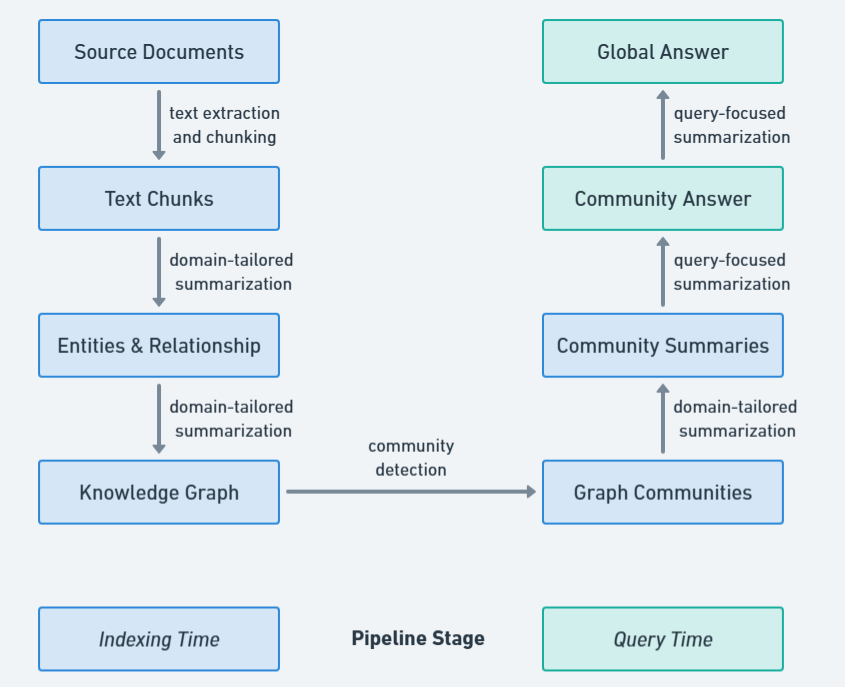
\includegraphics[width=0.8\textwidth]{images/graph-rag-pipeline.png}
	\caption{
		Alur kerja GraphRAG yang memanfaatkan indeks graf dan deteksi komunitas \cite{Edge2025LocalGlobalGraphRAG}
	}
	\label{fig:graphragpipeline}
\end{figure}

Penggunaan graf untuk memodelkan pengetahuan pada arsitektur RAG memberikan beberapa keuntungan dibandingkan RAG berbasis vektor.
Pada RAG konvensional berbasis vektor, sistem akan mengambil sekumpulan dokumen yang secara individu relevan dengan kueri \cite{Lewis2021RAGKnowledgeIntensiveNLP}.
Namun, saat kueri membutuhkan pemahaman \textit{dataset} secara global, RAG konvensional mengalami kesulitan karena basis pengetahuan disusun hanya sebagai potongan dokumen yang saling independen.
Dalam penelitian Edge et al. 2025 yang berjudul "\textit{From Local to Global: A GraphRAG Approach to Query-Focused Summarization}" mengintegrasikan model pengetahuan berbasis \textit{graph} dalam RAG \cite{Edge2025LocalGlobalGraphRAG}.
Alur kerja GraphRAG seperti pada \ref{fig:graphragpipeline} terdiri dari beberapa proses meliputi
\begin{enumerate}
	\item \textbf{\textit{Source Documents \textrightarrow{} Text Chunks}} \\
	      Pada proses ini, dokumen-dokumen awal dipecah menjadi potongan-potongan teks (\textit{text chunks}) dengan ukuran tertentu.
	      Menentukan ukuran dari potongan teks ini merupakan perkara krusial mengingat potongan teks yang panjang mengurangi jumlah kueri ke LLM (hemat biaya) tetapi dapat menurunkan kualitas pengambilan informasi di awal potongan \cite{Edge2025LocalGlobalGraphRAG}.

	\item \textbf{\textit{Text Chunks \textrightarrow{} Entities \& Relationships}} \\
	      LLM akan digunakan sebagai ekstraktor entitas penting, relasi antar entitas, dan deskripsi singkat untuk keduanya dari potongan teks sebelumnya.
	      Klaim yang berupa pernyataan faktual tentang entitas juga akan diekstrak oleh LLM \cite{Edge2025LocalGlobalGraphRAG}.
	      \textit{Prompt} LLM disesuaikan menggunakan teknik \textit{few-shot} yang memberikan beberapa contoh spesifik hasil yang diharapkan agar respons yang diberikan LLM sesuai \cite{LLMisFewShot2020}.

	\item \textbf{\textit{Entities Relationships \textrightarrow{} Knowledge Graph}} \\
	      Entitas, relasi, dan klaim yang telah diekstrak kemudian ditransformasi menjadi \textit{nodes} (entitas) dan \textit{edges} (relasi) dalam sebuah \textit{kowledge graph}.
	      Deskripsi entitas diagregasikan dengan entitas yang berupa \textit{node}.
	      Entitas, relasi, atau klaim dapat terdeteksi lebih dari satu kali karena proses ekstraksi dilakukan secara berulang dari banyak dokumen yang berbeda.
	      Banyaknya duplikasi relasi menjadi bobot dari \textit{edges} \cite{Edge2025LocalGlobalGraphRAG}.

	\item \textbf{\textit{Knowledge Graph \textrightarrow{} Graph Communities}} \\
	      Berdasarkan \textit{graph} yang telah terbentuk sebelumnya, komunitas akan dideteksi menggunaka algoritma tertentu yang bertujuan untuk memartisi \textit{graph} menjadi beberapa komunitas yang terdiri dari kumpulan \textit{nodes} yang terhubung dengan erat.
	      Dalam penelitian ini digunakan \textit{Leiden community detection} (Trag et al. 2019) secara hierarkis, mendeteksi sub-komunitas secara rekursif dalam setiap komunitas yang terdeteksi hingga mencapai komunitas yang tidak dapat lagi dipartisi \cite{Traag2019Leiden}.

	\item \textbf{\textit{Graph Communities \textrightarrow{} Community Summaries}} \\
	      Proses ini membuat ringkasan dari setiap komunitas dalam hierarki komunitas menggunakan metode tertentu.
	      Ringkasan ini secara independen berguna untuk memahami struktur global dan semantik \textit{dataset} serta dapat digunakan untuk memindai korpus tanpa adanya kueri tertentu.
	      Ringkasan berfungsi sebagai bagian dari indeks graf yang digunakan untuk menjawab kueri global \cite{Edge2025LocalGlobalGraphRAG}.

	\item \textbf{\textit{Community Summaries \textrightarrow{} Community Answers \textrightarrow{} Global Answer}} \\
	      Berdasarkan pertanyaan pengguna, ringkasan komunitas yang telah dibuat sebelumnya dapat digunakan untuk menghasilkan jawaban final melalui proses yang bertahap.
	      Ringkasan komunitas diacak dan dibagi menjadi potongan-potongan (\textit{chunks}) dengan ukuran token tertentu.
	      LLM menghasilkan jawaban sementara (\textit{intermediate answers}) dari \textit{chunks} ini secara paralel, beserta skor seberapa membantu jawaban tersebut (0-100).
	      Jawaban dengan skor 0 akan dibuang.
	      Jawaban sementara diurutkan berdasarkan skornya, lalu dimasukkan ke konteks baru LLM hingga batas token tercapai untuk menghasilkan jawaban global (\textit{global answer}) kepada pengguna \cite{Edge2025LocalGlobalGraphRAG}.
\end{enumerate}






\section{Dasar Teori}
\subsection{Kesehatan Mental}
Kesehatan mental, menurut definisi dari \textit{World Health Organization} (WHO), adalah sebuah kondisi kesejahteraan mental (\textit{state of mental well-being})
di mana setiap individu sadar akan potensi yang dimiliki, belajar dan bekerja dengan baik, dan memberikan kontribusi bagi komunitasnya \cite{WHO2022MentalHealth}.
Definisi tersebut menekankan bahwa kesehatan mental bukanlah sekadar kondisi bebas dari gangguan jiwa, melainkan sebuah fondasi yang memungkinkan seseorang untuk berpikir, belajar, merasakan emosi, berinteraksi dengan orang lain, dan menikmati hidup.
Kesehatan mental merupakan komponen yang tidak terpisahkan dengan kesehatan secara keseluruhan dan sama pentingnya dengan kesehatan fisik.

\subsection{\textit{Natural Language Processing}}
Pemrosesan bahasa alami (\textit{Natural Language Processing}, NLP) merupakan serangkaian teknik komputasi yang didorong secara teoritis untuk menganalisis dan merepresentasikan
teks alami pada beberapa tingkat analisis linguistik dengan tujuan mencapai pemrosesan bahasa seperti manusia untuk serangkaian tugas atau aplikasi \cite{Liddy2001NLP}.
Komputer tidak dapat mengerti bahasa manusia yang kompleks dan tidak pasti secara langsung, tetapi memerlukan sesuatu untuk menjadi penghubung antara keduanya.
NLP hadir sebagai cabang dari kecerdasan buatan (AI) yang berfungsi sebagai jembatan antara bahasa manusia yang kompleks dengan komputasi komputer yang terstruktur.
Tujuan utama dari NLP adalah memberdayakan komputer untuk memahami, menafsirkan, memanipulasi, dan menghasilkan bahasa manusia yang bermakna dan bermanfaat.

NLP dapat diklasifikasikan menjadi dua bagian, yaitu \textit{Natural Language Understanding} (NLU) dan \textit{Natural Language Generation} (NLG) \cite{Khurana2022AboutNLP}.
Berikut merupakan penjelasan dari NLU dan NLG.

\begin{enumerate}
	\item \textbf{\textit{Natural Language Understanding} (NLU)} \\
	      NLU memungkinkan komputer untuk memahami bahasa alami dan menganalisisnya dengan mengekstrak konsep, entitas, emosi, kata kunci, dll.
	      NLU berkaitan dengan ilmu bahasa (linguistik) yang berupa morfologi atau bentuk kata, leksikal atau makna kata, sintaksis atau susunan kalimat, semantik atau makna kalimat, \textit{discourse} atau hubungan antar kalimat, dan pragmatik atau makna kontekstual \cite{Khurana2022AboutNLP}.
	\item \textbf{\textit{Natural Language Generation} (NLG)} \\
	      NLG merupakan proses menghasilkan teks, dapat berupa kata, frasa, atau kalimat, yang bermakna dari representasi internal.
	      Proses ini terjadi dalam empat fase yaitu mengidentifikasi tujuan, merencanakan cara mencapai tujuan, mengevaluasi situasi dan sumber komunikasi yang tersedia, dan mewujudkan rencana sebagai teks \cite{Khurana2022AboutNLP}.
\end{enumerate}

Aplikasi NLP sangat luas dan meresap dalam kehidupan sehari-hari, mulai dari fungsionalitas mesin pencari, \textit{chatbot} layanan pelanggan, asisten digital seperti Bixby, Siri dan Alexa, hingga aplikasi khusus seperti analisis sentimen, mesin penerjemah otomatis, dan ekstraksi informasi dari dokumen.
Pada domain kesehatan mental, NLP telah menunjukkan potensi signifikan dalam menganalisis catatan klinis elektronik, unggahan di media sosial, dan respons survei untuk membantu dalam deteksi dini dan pemantauan kondisi seperti depresi, kecemasan, dan \textit{Post-Traumatic Stress Disorder} (PTSD) \cite{NLPonMentalHealth}.

\subsection{\textit{Machine Learning}}
Pembelajaran mesin (\textit{Machine Learning}, ML) adalah bidang AI yang fokus pada pembelajaran dengan mengembangkan algoritma terbaik untuk merepresentasikan data yang tersedia.
Berbeda dengan pemrograman klasik, di mana algoritma dapat dikodekan secara eksplisit menggunakan fitur yang diketahui,
ML menggunakan subset data untuk menghasilkan algoritma yang paling cocok untuk pola data tersebut \cite{choi2020IntroductionML_NN_DL}.
Inti dari ML adalah kemampuannya untuk secara otomatis menemukan pola dalam data dan menggunakan pola tersebut untuk membuat inferensi atau prediksi pada data baru yang belum pernah dilihat.

Algoritma ML membangun model matematis berdasarkan kumpulan data sampel, yang dikenal sebagai "data pelatihan" (\textit{training} data), untuk melakukan berbagai tugas seperti klasifikasi, regresi, atau pengelompokan.
Dalam ML terdapat beberapa metode pembelajaran yang umum digunakan, yaitu \textit{supervised} di mana model belajar dari data yang telah diberi label dengan output yang benar, \textit{unsupervised} di mana model belajar menemukan pola tersembunyi dari data tanpa label, dan \textit{reinforcement} di mana model belajar untuk membuat urutan keputusan dengan berinteraksi dengan lingkungannya untuk memaksimalkan imbalan kumulatif \cite{choi2020IntroductionML_NN_DL}.
Penerapan ML sangat luas, mencakup berbagai domain seperti penyaringan email spam, sistem rekomendasi, pengenalan objek, pengenalan ucapan, diagnosis medis berdasarkan data pasien, dan analisis pasar keuangan untuk prediksi tren.
ML menjadi sangat berguna dalam situasi di mana perancangan dan pengkodean algoritma konvensional yang eksplisit untuk melakukan tugas tertentu dianggap sulit atau tidak praktis karena kompleksitas masalah atau sifat data yang dinamis.


\subsection{\textit{Deep Learning}}
Pembelajaran mendalam (\textit{Deep Learning, DL}) merupakan sebuah pendekatan dalam \textit{Machine learning} yang berusaha mempelajari representasi data melalui struktur model yang terdiri dari banyak lapisan (\textit{layers}) \cite{IanGoodfellow2016DeepLearning}.
Beberapa algoritma pembelajaran yang dikembangkan, awalnya dikembangkan sebagai model komputasi dari pembelajaran biologis yang meniru cara otak bekerja.
Maka dari itu, nama lain dari \textit{deep learning} adalah jaringan saraf tiruan (\textit{Artificial Neural Network}, ANN) \cite{IanGoodfellow2016DeepLearning}.
Jaringan tersebut digunakan untuk mempelajari representasi data dengan berbagai tingkat abstraksi.
Istilah mendalam (\textit{deep}) merujuk pada kedalaman atau banyaknya lapisan dalam jaringan saraf ini.
Setiap lapisan dalam arsitektur DL menerima output dari lapisan sebelumnya, mentransformasikannya, dan meneruskannya ke lapisan berikutnya, secara bertahap mengekstraksi fitur-fitur yang semakin kompleks dan relevan dari data input mentah \cite{IanGoodfellow2016DeepLearning}.

Sebagai subset dari \textit{Machine Learning} (ML), yang juga merupakan subset dari AI, DL memiliki perbedaan signifikan dibandingkan dengan ML.
DL memiliki kemampuan \textit{feature engineering} secara otomatis.
ML konvensional sering kali memerlukan intervensi manusia untuk merancang dan memilih fitur-fitur input yang relevan dari data, model DL dapat secara mandiri mempelajari hierarki fitur yang optimal langsung dari data mentah, seperti piksel dalam gambar atau kata-kata dalam teks \cite{IanGoodfellow2016DeepLearning}.
Aplikasi DL telah merambah berbagai bidang, termasuk pengenalan gambar dan ucapan, deteksi objek dalam video, pemrosesan bahasa alami untuk terjemahan dan pemahaman, serta pengembangan kendaraan otonom.


\subsection{\textit{Large Language Model}}
Model bahasa besar (\textit{Large Language Model}, LLM) merupakan model bahasa berskala besar yang mampu memahami, memprediksi, dan menghasilkan bahasa manusia secara alami dan kontekstual \cite{Chang2024SurveyonLLM}.
LLM merupakan bentuk lanjutan dari \textit{language models} (LMs), yang secara umum adalah sistem komputasi yang mempelajari probabilitas urutan kata dalam teks.
Model bahasa awal seperti \textit{n-gram models} memprediksi kata berikutnya berdasarkan konteks kata-kata sebelumnya, namun memiliki keterbatasan seperti ketidakmampuan menangani kata yang jarang muncul, kecenderungan \textit{overfitting}, serta kesulitan dalam memahami struktur linguistik yang kompleks.
LLM hadir untuk mengatasi tantangan tersebut dengan memanfaatkan arsitektur modern dan kapasitas pembelajaran yang jauh lebih besar \cite{Chang2024SurveyonLLM}.

Keunggulan lain dari LLM terletak pada kemampuan \textit{in-context learning}, yaitu kemampuan untuk melakukan adaptasi dan menyelesaikan berbagai tugas hanya dari petunjuk yang diberikan dalam bentuk \textit{prompt}, tanpa perlu pelatihan ulang secara eksplisit.
LLM dapat "belajar" dari konteks input yang diberikan pengguna untuk memberikan respons yang relevan dan akurat.
Fitur ini membuat LLM sangat fleksibel dan dapat digunakan untuk berbagai keperluan, mulai dari menjawab pertanyaan, membuat ringkasan, menerjemahkan teks, menulis kode program, hingga mengekstrak entitas dari sebuah dokumen \cite{Chang2024SurveyonLLM}.

\subsection{Gemini}
Gemini adalah famili model AI multimoda yang dikembangkan oleh Google DeepMind.
Model Gemini dibangun berdasarkan arsitektur transformer \textit{decoders}.
Model ini dilatih dengan data multimoda dan multilingual yang berasal dari \textit{website}, buku, dan kode, termasuk juga gambar, audio, dan video \cite{saeidnia2023welcomeGemini}.
Saat penelitian dilakukan, Gemini telah berada pada versi 2.5 yang menggunakan arsitektur  \textit{sparse mixture-of-experts} (MoE) \textit{transformer}.
Gemini 2.5 mendukung input konteks dengan panjang lebih dari 1 juta token yang memungkinkan untuk memahami data dengan cakupan yang luas \cite{comanici2025gemini2.5}.



\subsection{GPT}
\textit{Generative Pre-trained Transformer} (GPT) adalah \textit{language model} berbasis arsitektur transformer yang dikembangkan oleh OpenAI sejak tahun 2018 saat rilis model transformer pertamanya.
Saat penelitian ini dilakukan, OpenAI telah memperbarui model GPT hingga generasi keempat seperti gpt-4.1.
Model ini dilatih secara unsupervised pada kumpulan data dalam jumlah besar yang berasal dari \textit{website} publik, kode dan data matematis, serta data multimodal seperti gambar, audio, dan video.
Pelatihan tersebut bertujuan untuk memahami pola bahasa alami, lalu digunakan untuk menghasilkan teks baru yang koheren.
GPT bekerja dengan mekanisme \textit{self-attention} yang memungkinkan model memahami konteks panjang dalam sebuah teks, sehingga mampu menghasilkan jawaban yang relevan dan konsisten \cite{hurst2024gpt4o}.

\subsection{\textit{Retrieval-Augmented Generation}}
\textit{Retrieval-Augmented Generation} (RAG) adalah teknik yang menggabungkan kekuatan \textit{Large Language Model} (LLM) dengan sistem pengambilan (\textit{retrieval}) informasi dari sumber eksternal (seperti basis pengetahuan atau dokumen) untuk meningkatkan akurasi, ketepatan, dan kedalaman pengetahuan dalam tugas \textit{knowledge-intensive} seperti tanya-jawab terbuka atau penjelasan faktual.
Tujuan utama RAG adalah untuk mengatasi beberapa keterbatasan yang melekat pada LLM standar, seperti kecenderungan untuk menghasilkan informasi yang tidak akurat atau "berhalusinasi", menyajikan pengetahuan yang tidak relevan, atau kurangnya kemampuan untuk menyediakan sumber atau justifikasi atas informasi yang dihasilkannya \cite{Lewis2021RAGKnowledgeIntensiveNLP}.


\subsection{Token}
Dalam bidang \textit{Natural Language Processing} (NLP), token merujuk pada satuan terkecil dari teks yang dapat dikenali dan diproses oleh sistem komputasi bahasa.
Token dapat berupa kata, bagian dari kata (\textit{subword}), tanda baca, atau bahkan karakter individual, tergantung pada strategi tokenisasi yang digunakan \cite{Jurafsky2023SpeechLangageProcessing}.
Proses pemecahan teks menjadi token disebut tokenisasi, dan merupakan tahap awal penting dalam \textit{pipeline} pemrosesan bahasa alami.
Dalam model \textit{Large Language Model} seperti GPT atau BERT, tokenisasi umumnya dilakukan dengan pendekatan berbasis \textit{subword}, seperti \textit{Byte Pair Encoding} (BPE) atau WordPiece, yang memungkinkan model mengenali dan memproses kata-kata baru atau langka dengan efisien \cite{bostrom2020BytePairWordPieceToken}.
Tokenisasi berbasis \textit{subword} menyusun token dari unit-unit kata yang lebih kecil sehingga kosakata tetap terbatas namun tetap mencakup variasi linguistik yang luas.
Misalnya, kata "memperjuangkan" dapat dipecah menjadi beberapa token seperti "mem", "perjuang", dan "kan".


\subsection{Vektor}
Vektor adalah sebuah objek matematis yang memiliki dua karakteristik utama yaitu magnitudo (besar) dan arah.
Secara fundamental, sebuah vektor dapat direpresentasikan sebagai sebuah larik (\textit{array}) terurut yang berisi angka.
Vektor tersebut merupakan elemen dari suatu ruang vektor (\textit{vector space}) yang merupakan himpunan objek yang memiliki operasi penjumlahan dan perkalian skalar serta memenuhi sejumlah aksioma tertentu \cite{strang2009IntroductionLinearAlgebra}.
Sebuah vektor dalam ruang berdimensi $n$ dapat direpresentasikan sebagai barisan terurut dari $n$ bilangan real seperti pada Persamaan \ref{eq:vector}.
\def\V{
	\begin{bmatrix}
		v_1    \\
		v_2    \\
		\vdots \\
		v_n
	\end{bmatrix}
}

\begin{equation}
	\mathbf{v} = \V \in \mathbb{R}^n
	\label{eq:vector}
\end{equation}%
dengan $v_1, v_2, \cdots, v_n$ adalah komponen-komponen dari vektor $\mathbf{v}$ dan $n$ adalah dimensi ruang tempat vektor tersebut berada.
Dalam konteks kecerdasan buatan, vektor biasanya digunakan untuk merepresentasikan objek kompleks seperti teks, gambar, atau video ke dalam bentuk numerik yang dapat diproses oleh mesin.


\subsection{\textit{Cosine Similarity}}
Kesamaan kosinus (\textit{cosine similarity}) merupakan salah satu metrik matematis untuk yang digunakan untuk mengukur tingkat kemiripan antara dua vektor \textit{non-zero}.
Secara fundamental, metrik ini menghitung nilai kosinus dari sudut yang dibentuk oleh dua vektor tersebut.
Fokus utama dari \textit{cosine similarity} adalah pada orientasi atau arah vektor-vektor tersebut dan mengabaikan besar atau magnitudonya \cite{Xia2015CosineSimilarity}.
Hal ini menjadikannya sangat berguna dalam konteks di mana besaran absolut dari vektor kurang relevan dibandingkan dengan "arah" atau "profil" relatifnya.
Secara matematis, formula untuk menghitung nilai \textit{cosine similarity} dapat diungkapkan dengan Persamaan \ref{eq:cosine-similarity}.

\begin{equation}
	\text{$Similarity$}(\vec{A}, \vec{B}) = \cos{(\theta)} = \frac{\vec{A} \cdot \vec{B}}{\|\vec{A}\| \|\vec{B}\|} = \frac{\sum_{i=1}^{n} A_i B_i}{\sqrt{\sum_{i=1}^{n} A_i^2} \sqrt{\sum_{i=1}^{n} B_i^2}}
	\label{eq:cosine-similarity}
\end{equation}%
dengan $\vec{A} \cdot \vec{B}$ adalah \textit{dot product} dari vektor $A$ dan $B$, $\|\vec{A}\|$ adalah magnitudo atau besar dari vektor $A$ dan $\|\vec{B}\|$ adalah magnitudo atau besar dari vektor $B$.
\textit{Dot product} $\vec{A} \cdot \vec{B}$ dilakukan dengan mengalikan komponen-komponen yang bersesuaian dari kedua vektor kemudian menjumlahkan hasilnya.
Magnitudo dari sebuah vektor dihitung sebagai akar kuadrat dari jumlah kuadrat setiap komponennya.
Nilai \textit{cosine similarity} akan selalu berada pada rentang $-1$ hingga $1$.
Nilai $1$ menunjukkan bahwa kedua vektor memiliki orientasi yang sama persis atau sudut yang dibentuk keduanya 0 derajat.
Nilai $0$ menunjukkan bahwa kedua vektor ortogonal atau saling tegak lurus (sudut 90 derajat) yang sering diartikan sebagai tidak adanya kesamaan orientasi.
Nilai $-1$ menunjukkan bahwa kedua vektor memiliki orientasi yang berlawanan arah (sudut 180 derajat).
Dua buah vektor dikatakan mirip apabila nilai \textit{cosine similarity} antar keduanya mendekati $1$.


\subsection{\textit{Vector Embedding}}
\textit{Vector embedding} merupakan representasi numerik dari sebuah data, terutama yang tidak terstruktur seperti teks, gambar, audio, atau video.
Pada prinsipnya \textit{vector embedding} bekerja dengan melakukan transformasi data ke dalam bentuk vektor berdimensi tinggi.
Bentuk vektor tersebut merepresentasikan fitur atau karakteristik dari objek asli, seperti makna dalam teks, objek dalam gambar, atau suara dalam audio.
Dalam konteks NLP \textit{embedding} digunakan untuk menangkap hubungan semantik, sintaksis, atau kontekstual yang mendasari sebuah teks.
Hal tersebut membuat hubungan antar objek seperti kemiripan semantik teks dapat dianalisis secara matematis \cite{Singh2023EmbeddingVectorAndVectorDB}.

Proses pembentukan \textit{vector embedding} biasanya melibatkan model \textit{machine learning} tradisional seperti Word2Vec dan GloVe atau model berbasis \textit{transformer} yang lebih modern seperti BERT, GPT, dan Gemini.
Model-model tersebut telah dilatih untuk menghasilkan nilai-nilai dalam \textit{vector embedding} berdasarkan makna atau konteks setiap unit data.
Model tradisional seperti GloVe bekerja dengan mentransformasi setiap kata menjadi 1 representasi vektor unik tanpa memperhatikan bagai mana kata tersebut digunakan dalam kalimat.
Sebaliknya, model yang lebih modern seperti BERT, GPT, dan Gemini mampu menghasilkan representasi vektor yang berbeda untuk kata yang sama tergantung pada konteks spesifik kalimat di mana kata tersebut muncul.

\subsection{\textit{Full-Text Search}}
Dalam konteks \textit{information retrieval}, \textit{full-text search} merujuk kepada teknik untuk melakukan pencarian keseluruhan konten tekstual dari sebuah atau koleksi dokumen yang tersimpan.
\textit{Full-text search} adalah jenis pencarian yang dilakukan dengan mencocokkan istilah (\textit{terms}) yang terkandung dalam kueri pencarian dengan \textit{terms} dalam setiap dokumen dalam basis data, kemudian hasilnya di-\textit{ranking} dengan algoritma tertentu.
Jenis pencarian ini banyak digunakan di berbagai bidang, mencakup pencarian bahasa alami yang banyak dijumpai pada mesin pencari, pencarian situs web, dan banyak basis data \cite{beall2008weaknesses}.
Keunggulan utama dari metode pencarian ini adalah kemampuannya dalam menangani variasi teks, termasuk \textit{stemming}, \textit{stopwords}, dan peringkat relevansi hasil.
Misalnya, sistem dapat mendeteksi bahwa kata “berlari” dan “lari” memiliki makna dasar yang sama, sehingga hasil pencarian menjadi lebih akurat.
Dalam implementasi modern, \textit{full-text search} biasanya dilengkapi dengan teknik seperti \textit{inverted index}, \textit{ranking model}, dan skor relevansi \cite{mongodb2025fulltext}.

\subsection{\textit{Vector Database}}
Basis data vektor (\textit{vector database}) adalah salah satu jenis basis data yang dirancang khusus untuk secara efektif mengelola data yang direpresentasikan sebagai vektor berdimensi tinggi.
Vektor-vektor tersebut merupakan representasi numeris dari fitur atau atribut suatu objek yang umumnya dibentuk melalui proses \textit{vector embedding}.
Setiap vektor dapat memiliki puluhan hingga ribuan dimensi tergantung pada kompleksitas data yang direpresentasikan.
Vektor-vektor ini kemudian sering kali dikelompokkan atau diindeks berdasarkan kedekatan mereka dalam ruang vektor multidimensi untuk memudahkan dalam pencarian \cite{Han2023VectorDB_ANN_SimilaritySearch}.

Basis vektor berbeda secara fundamental dengan basis data relasional berbasis baris dan kolom, basis data ini unggul dalam menangani volume besar data tidak terstruktur yang telah ditransformasikan menjadi representasi vektor padat berdimensi tinggi.
Fitur kueri pencarian kemiripan (\textit{similarity search}) menjadikannya sangat unggul dibandingkan basis data lain karena fitur tersebut merupakan operasi krusial bagi banyak aplikasi AI.
Umumnya basis data vektor seperti ChromaDB, Pinecone, Melvis, dll. mendukung algoritma \textit{Approximate Nearest Neighbor} (ANN) yang efisien untuk menemukan vektor-vektor yang paling mirip dengan vektor kueri dalam data yang sangat besar \cite{Han2023VectorDB_ANN_SimilaritySearch}.
Hal tersebut menjadikannya pilihan utama saat berinteraksi dengan data berbentuk vektor.

\subsection{\textit{Graph Database}}
Basis data graf (\textit{graph database}) adalah basis data yang dirancang untuk secara efisien mengelola data yang dimodelkan dalam bentuk graf.
Struktur data pada basis data graf secara fundamental terdiri atas \textit{node} atau \textit{vertex} yang merepresentasikan sebuah entitas atau objek dan \textit{edge} yang merepresentasikan koneksi atau relasi antar node tersebut.
Baik \textit{node}, maupun \textit{edge} dapat memiliki properti yang menyimpan atribut atau metadata yang dapat berisi deskripsi dari entitas atau relasi tersebut \cite{Paul2019GraphDB}.
Salah satu keunggulan dari basis data graf adalah adanya konsep \textit{index-free adjacency} yang berarti setiap \textit{node} dapat secara langsung mengetahui dan dapat mengakses \textit{node} lain yang berhubungan tanpa harus menggunakan indeks tambahan seperti pada basis data relasional.
Hal tersebut mempercepat performa pencarian hubungan antar \textit{node} dan memungkinkan algoritma seperti \textit{graph traversal} yang efisien \cite{Paul2019GraphDB}.

\subsection{\textit{Knowledge Graph}}
Konsep Graf Pengetahuan (\textit{Knowledge Graph}, KG) pertama kali diperkenalkan secara luas oleh Google pada tahun 2012 melalui proyek Google \textit{Knowledge Graph} untuk meningkatkan relevansi hasil pencarian dan pengalaman pencarian pengguna \cite{Singhal2012IntroducingKnowledgeGraph}.
Bermula dari itu, banyak perusahaan dan institusi mengembangkan KG mereka sendiri seperti Bing dengan Stori, DBpedia, YAGO, Wikidata, dan Freebase sebagai bagian dari \textit{semantic web} \cite{Paulheim2016KnowledgeGraphSurvei}.
\textit{Knowledge Graph} adalah representasi semantik terstruktur dari pengetahuan yang memodelkan entitas (seperti orang, tempat, organisasi, dll.) dan hubungan antar entitas dalam bentuk graf.
Setiap entitas direpresentasikan sebagai \textit{node} dan relasi antar entitas direpresentasikan sebagai \textit{edge} \cite{Chen2020ReviewKnowldgeReasoningOverKnowledgeGraph}.
Secara matematis, sebuah struktur KG dapat direpresentasikan dengan Persamaan \ref{eq:knowledge-graph}
\begin{equation}
	\text{$KG$} = \langle E, R, T \rangle
	\label{eq:knowledge-graph}
\end{equation}%
dengan $E$ adalah himpunan semua \textit{node} atau entitas dalam pengetahuan, $R$ adalah himpunan semua relasi, dan $T$ adalah himpunan triplet yang merepresentasikan fakta.
$T$ dapat dinyatakan secara matematis, seperti pada Persamaan \ref{eq:triple-in-kg}

\begin{equation}
	T = \{(h,r,t) \mid h,t \in E, r \in R\}
	\label{eq:triple-in-kg}
\end{equation}

Setiap triplet $T$ terdiri dari tiga bagian yaitu $h$ (\textit{head}) adalah entitas asal, $r$ adalah relasi, dan $t$ (\textit{tail}) adalah entitas tujuan.

\subsection{\textit{Knowledge Extraction}}
Ekstraksi pengetahuan (\textit{Knowledge Extraction}, KE) merupakan proses sistematis untuk mengidentifikasi dan mengekstrak informasi bermakna dari data tidak terstruktur atau semi terstruktur seperti teks untuk direpresentasikan ke dalam bentuk terstruktur yang dapat dipahami oleh mesin.
Dalam konteks \textit{Knowledge Graph}, sumber data yang berupa dokumen akan diekstrak menjadi bentuk triplet (subjek-predikat-objek) yang akan membentuk KG.
Pada praktiknya proses ekstraksi ini terdiri dari ekstraksi entitas, relasi antar entitas, dan klasifikasi entitas.
Proses ini merupakan tahap awal yang krusial dalam konstruksi KG karena akan menentukan kualitas representasi pengetahuan oleh \textit{Knowledge Graph} \cite{Choi2025KnowledgeGraphConstruction}.

\subsection{\textit{Knowledge Retrieval}}
Pengambilan pengetahuan (\textit{Knowledge Retrieval}, KR) merupakan proses pencarian dan pengambilan pengetahuan secara sistematis dari basis data pengetahuan seperti \textit{Knowledge Graph} \cite{Yao2007KnowledgeRetrieval}.
Dalam konteks KG, proses pengambilan ini memungkinkan suatu sistem untuk melakukan inferensi logis dan menjawab kueri secara presisi dan benar.
Penekanan utama dalam \textit{Knowledge Retrieval} adalah pada pengambilan pengetahuan yaitu representasi formal pengetahuan yang dapat diolah untuk penalaran, bukan sekadar pengambilan data mentah atau informasi yang terkait dengan kueri.
KR bertujuan untuk mengambil makna dan hubungan terstruktur yang kemudian dapat dimanfaatkan untuk tugas lain yang lebih kompleks.

\subsection{\textit{Precision}}
\textit{Precision} (presisi) merupakan metrik yang mengukur seberapa banyak item yang berhasil diidentifikasi (\textit{retrieved}) yang benar-benar relevan.
Metrik ini juga dikenal sebagai \textit{confidence} dalam bidang \textit{data mining} dan menjadi fokus utama dalam \textit{information retrieval} dan \textit{machine learning} untuk mengukur keyakinan pada hasil prediksi.
Presisi menunjukkan proporsi kasus positif yang diprediksi dengan positif yang sebenarnya \cite{powers2020evaluationprecisionrecallfmeasure}.
Definisi \textit{Precision} diberikan pada Persamaan \ref{eq:precision}.

\begin{equation}
	\label{eq:precision}
	Precision = \frac{TP}{TP + FP}
	= \frac{\textit{Relevant items retrieved}}{\textit{Retrieved items}}
\end{equation}%
dengan:
\begin{itemize}
	\item $TP$ adalah \textit{True Positives}, yaitu jumlah prediksi positif yang benar.
	\item $FP$ adalah \textit{False Positives}, yaitu jumlah prediksi positif yang salah.
\end{itemize}

Presisi memiliki rentang nilai antara 0 dan 1 ($0 \leq Precision \leq 1$).
Nilai presisi mendekati 1 menunjukkan banyak \textit{item} relevan dari semua \textit{item} yang diambil.
Nilai presisi mendekati 0 berarti banyak \textit{noise} atau \textit{item} tidak relevan yang diambil.
Dalam kasus RAG, presisi berarti proporsi banyaknya informasi relevan dari semua informasi yang dihasilkan dibandingkan dengan total informasi yang dihasilkan.

\subsection{\textit{Recall}}

\textit{Recall} merupakan metrik yang mengukur seberapa banyak item relevan yang berhasil diidentifikasi dari semua item yang relevan.
Metrik ini juga dikenal sebagai \textit{sensitivity} atau \textit{True Positive Rate} (TPR).
\textit{Recall} menunjukkan proporsi kasus positif yang diprediksi dengan total kasus positif yang seharusnya muncul \cite{powers2020evaluationprecisionrecallfmeasure}.
Definisi \textit{Recall} diberikan pada Persamaan \ref{eq:recall}.

\begin{equation}
	\label{eq:recall}
	Recall = \frac{TP}{TP + FN} = \frac{\textit{Relevant items retrieved}}{\textit{Relevant items}}
\end{equation}%
dengan:
\begin{itemize}
	\item $TP$ adalah \textit{True Positives}, yaitu jumlah prediksi positif yang benar.
	\item $FN$ adalah \textit{False Negatives}, yaitu jumlah kasus positif yang gagal diprediksi (salah diprediksi negatif).
\end{itemize}

\textit{Recall} memiliki rentang nilai antara 0 dan 1 ($0 \leq Recall \leq 1$).
Nilai \textit{recall} mendekati 1 menunjukkan banyak \textit{item} relevan yang diambil dari semua kemungkinan \textit{item} relevan.
Nilai \textit{recall} mendekati 0 menunjukkan sedikit \textit{item} relevan yang diambil dari semua kemungkinan \textit{item} relevan.
Dalam kasus RAG \textit{recall} berarti proporsi banyaknya informasi relevan dari semua informasi yang dihasilkan dibandingkan dengan total informasi relevan yang seharusnya muncul.


\subsection{\textit{Mean Reciprocal Rank} (MRR)}
Metrik \textit{Reciprocal Rank} (RR) menghitung kebalikan dari peringkat (\textit{rank}) di mana dokumen relevan pertama ditemukan.
RR bernilai 1 jika dokumen relevan ditemukan pada peringkat 1,  0,5 jika ditemukan pada peringkat 2,  0,33 pada peringkat 3, dan seterusnya.
Ketika dirata-ratakan di seluruh kueri, ukuran ini disebut \textit{Mean Reciprocal Rank} (MRR) \cite{craswell2016meanMRR}.
MRR didefinisikan dalam Persamaan \ref{eq:mrr}

\begin{equation}
	\label{eq:mrr}
	\mathrm{MRR} = \frac{1}{N} \sum_{i=1}^{N} \frac{1}{\text{rank}_i}
\end{equation}

MRR memiliki rentang nilai antara 0 dan 1 ($0 \leq \mathrm{MRR} \leq 1$).
Nilai 1 adalah skor sempurna, yang berarti untuk setiap kueri, dokumen relevan pertama selalu muncul di peringkat pertama.
Nilai 0 berarti sistem tidak pernah berhasil menemukan dokumen relevan untuk kueri apa pun.
Dalam konteks RAG, MRR menunjukkan performa \textit{retriever} dalam memprioritaskan urutan munculnya konteks yang relevan.
Hal tersebut cukup krusial karena beberapa LLM memiliki kecenderungan memprioritaskan informasi yang muncul di awal.

\subsection{\textit{Retrieval-Augmented Generation Assessment} (RAGAS) \textit{Framework}}

RAGAS (\textit{Retrieval-Augmented Generation Assessment}) adalah sebuah kerangka kerja yang dirancang untuk mengevaluasi sistem AI yang menggunakan arsitektur \textit{Retrieval-Augmented Generation} (RAG).
Tujuan utamanya adalah untuk mengatasi tantangan dalam menilai kualitas \textit{pipeline} RAG, yang terdiri dari komponen pengambilan (\textit{retrieval}) dan generasi (\textit{generation}).
Kerangka kerja ini menyediakan serangkaian metrik otomatis yang dapat mengukur berbagai aspek kinerja berbasis LLM sehingga mampu untuk mengevaluasi data dalam bentuk bahasa alami.
Dengan demikian, RAGAS memungkinkan pengembang untuk secara efisien mendiagnosis kelemahan, baik pada kemampuan sistem untuk menemukan informasi yang relevan, maupun pada kemampuannya untuk menghasilkan jawaban yang akurat dan koheren dari informasi tersebut \cite{es2024ragas}.

Untuk memberikan evaluasi yang komprehensif, RAGAS menyediakan beberapa metrik utama untuk mengevaluasi sistem RAG.

\begin{enumerate}
	\item \textbf{\textit{Faithfulness}} \\
	      Metrik pertama adalah \textit{faithfulness} atau kepatuhan.
	      \textit{Faithfulness} adalah metrik krusial yang mengukur konsistensi faktual jawaban yang dihasilkan terhadap konteks yang diambil.
	      Metrik ini memastikan bahwa model tidak berhalusinasi dengan memverifikasi bahwa setiap klaim dalam jawaban didukung oleh sumber yang diberikan.
	      Rentang nilai \textit{faithfulness} adalah dari 0 hingga 1, di mana skor 1 menunjukkan kepatuhan faktual yang sempurna (semua klaim terdukung), dan skor 0 menunjukkan jawaban sepenuhnya berhalusinasi atau tidak relevan dengan konteks.
	\item \textbf{\textit{Response Relevancy}} \\
	      \textit{Response Relevancy} menilai seberapa relevan jawaban terhadap pertanyaan asli.
	      Jawaban yang tidak lengkap atau mengandung informasi berlebihan yang tidak diminta akan dikenakan penalti.
	      Metrik ini memiliki rentang nilai dari 0 hingga 1.
	      Semakin tinggi nilainya menunjukkan respons selaras dengan pertanyaan, sedangkan semakin kecil nilainya menunjukkan respons kurang lengkap atau mengandung informasi yang redundan.
	      Metrik ini tidak mengukur kebenaran, melainkan fokus pada ketepatan dalam menjawab pertanyaan.
	\item \textbf{\textit{Answer Similarity}} \\
	      \textit{Answer Similarity} secara spesifik mengukur kemiripan semantik antara jawaban yang dihasilkan dan jawaban referensi, biasanya dihitung menggunakan \textit{cosine similarity} dari \textit{embedding} kedua jawaban tersebut.
	      Skala nilainya berkisar dari 0 (tidak ada kemiripan makna) hingga 1 (makna identik secara semantik).
	\item \textbf{\textit{Correctness}} \\
	      Selanjutnya, \textit{Correctness} mengevaluasi keakuratan jawaban secara keseluruhan dengan membandingkannya dengan jawaban referensi (\textit{ground truth}).
	      Metrik ini bergantung pada \textit{ground truth} dan jawaban, dengan skor berkisar antara 0 hingga 1.
	      Skor yang lebih tinggi menunjukkan kesesuaian yang lebih dekat antara jawaban yang dihasilkan dan kebenaran dasar, yang menandakan ketepatan yang lebih baik.
\end{enumerate}


\section{Analisis Perbandingan Metode}

Dalam tinjauan pustaka telah diulas berbagai metode untuk mengembangkan \textit{chatbot}.
Komparasi dari masing-masing metode tersebut terdapat pada Tabel \ref{tab:method-comparision}.

\begin{sidewaystable}
	\centering
	\caption{Ringkasan dan Perbandingan Metode Pengembangan \textit{Chatbot}}
	\label{tab:method-comparision}
	\begin{tabularx}{\textheight}{|X|p{8.5cm}|p{8.5cm}|}
		\hline
		\textbf{Metode} & \textbf{Kelebihan} & \textbf{Kekurangan} \\
		\hline\hline

		\textbf{\textit{Fine-Tuning LLM}: }
		Melatih lebih lanjut sebuah \textit{Large Language Model} (LLM) yang sudah ada dengan menggunakan \textit{dataset} spesifik domain.
		Tujuannya adalah untuk mengadaptasi pengetahuan dan gaya respons model agar sesuai dengan kebutuhan.
		                &
		\begin{enumerate}[leftmargin=*]
			\item Menghasilkan respons yang sangat relevan dan akurat untuk domain spesifik.
			\item Gaya bahasa dan "kepribadian" \textit{chatbot} dapat disesuaikan.
			\item Latensi sama dengan \textit{base} model.
		\end{enumerate}
		                &
		\begin{enumerate}[leftmargin=*]
			\item Membutuhkan \textit{dataset} pelatihan yang besar dan berkualitas tinggi.
			\item Prosesnya mahal secara komputasi dan memakan waktu.
			\item Pengetahuan terbatas pada saat pelatihan.
			\item Pengetahuan baru ditambahkan dengan melatih ulang model.
		\end{enumerate}
		\\
		\hline
		\textbf{\textit{Prompt Engineering LLM}: }
		Merancang dan menyusun instruksi (\textit{prompt}) yang detail dan terstruktur untuk mengarahkan LLM agar memberikan respons yang diinginkan tanpa mengubah model itu sendiri.
		                &
		\begin{enumerate}[leftmargin=*]
			\item Tidak memerlukan pelatihan ulang.
			\item Biaya rendah dan fleksibel.
			\item Sangat mudah dilakukan pembaruan sesuai kebutuhan.
		\end{enumerate}
		                &
		\begin{enumerate}[leftmargin=*]
			\item Performa sangat tergantung kualitas \textit{prompt}.
			\item Konsistensi jawaban tidak selalu terjamin.
			\item Sulit untuk menangani domain yang sangat spesifik.
			\item Tidak \textit{scalable} untuk domain pengetahuan masif.
		\end{enumerate}
		\\
		\hline
		\textbf{\textit{Retrieval-Augmented Generation} Konvensional: }
		Menggabungkan LLM dengan sistem pencarian informasi dari basis data eksternal (misalnya, dokumen teks).
		Sebelum menjawab, sistem mencari informasi relevan terlebih dahulu, lalu memberikannya sebagai konteks bagi LLM.
		                &
		\begin{enumerate}[leftmargin=*]
			\item Mengurangi halusinasi karena jawaban didasarkan pada sumber nyata.
			\item Memudahkan pembaruan informasi tanpa proses \textit{training} ulang.
		\end{enumerate}
		                &
		\begin{enumerate}[leftmargin=*]
			\item Kualitas jawaban sangat bergantung pada kualitas \textit{retriever}.
			\item Butuh \textit{pipeline} tambahan untuk pencarian data yang dapat menambah latensi.
		\end{enumerate}
		\\
		\hline
		\textbf{\textit{Retrieval-Augmented Generation} dengan \textit{Knowledge Graph}: }
		Varian dari RAG yang menggunakan \textit{Knowledge Graph} (KG) sebagai basis data eksternal.
		KG merepresentasikan informasi sebagai entitas dan hubungan yang terstruktur, memberikan konteks yang lebih kaya kepada LLM.
		                &
		\begin{enumerate}[leftmargin=*]
			\item Lebih terstruktur dalam memodelkan informasi dibanding dokumen teks biasa.
			\item Mendukung pencarian dengan konteks yang lebih luas.
			\item Memperkuat konteks relasional antar data.
			\item Dapat meng-\textit{update} informasi tanpa \textit{retraining}.
		\end{enumerate}
		                &
		\begin{enumerate}[leftmargin=*]
			\item Pembuatan \textit{Knowledge Graph} memerlukan pemodelan yang optimal.
			\item Kompleksitas implementasi tinggi.
		\end{enumerate}
		\\
		\hline
	\end{tabularx}
\end{sidewaystable}

\pagebreak
Metode \textit{Fine-Tuning} LLM menawarkan beberapa keunggulan utama, seperti kemampuan untuk menghasilkan respons yang sangat relevan dan akurat untuk domain spesifik.
Selain itu, metode ini memungkinkan pengembang untuk menyesuaikan gaya bahasa dan "kepribadian" \textit{chatbot}, yang didukung oleh latensi yang lebih rendah karena tidak memerlukan konteks eksternal saat inferensi.

Namun, di balik kelebihannya, terdapat kekurangan yang signifikan, proses \textit{fine-tuning} membutuhkan \textit{dataset} pelatihan yang besar dan berkualitas tinggi, menjadikannya mahal dan memakan waktu secara komputasi.
Pengetahuan yang ditanamkan ke dalam model juga bersifat statis, sehingga sulit untuk diperbarui tanpa melalui proses pelatihan ulang yang intensif.
Kelemahan yang paling krusial adalah metode ini masih rentan terhadap "halusinasi", yaitu memberikan informasi yang salah atau tidak faktual.

Dalam konteks yang sangat sensitif seperti layanan kesehatan mental, risiko halusinasi dari metode \textit{fine-tuning} menjadi opsi yang riskan.
Oleh karena itu, metode RAG berbasis \textit{\textit{Knowledge Graph}} muncul sebagai solusi yang lebih unggul.
Dengan mendasarkan jawaban pada basis data terstruktur yang memetakan entitas dan relasinya, RAG dengan KG secara signifikan mengurangi ambiguitas dan meningkatkan akurasi fakta.
Kemampuannya untuk melakukan penalaran yang kompleks berdasarkan sumber terverifikasi menjadikannya pilihan yang lebih aman dan andal untuk membangun \textit{chatbot} kesehatan mental yang bertanggung jawab.

\cleardoublepage \phantomsection
\chapter{Metode Penelitian}

Bab ini menyajikan ulasan mengenai alat dan bahan yang akan dipakai untuk menyelesaikan tugas akhir ini.
Alat dan bahan tersebut meliputi perangkat keras, perangkat lunak, dan data yang digunakan.
Selanjutnya akan dijelaskan mengenai rancangan serta langkah-langkah metodologis yang akan diimplementasikan dalam pelaksanaan penelitian ini.

\section{Alat dan Bahan Tugas Akhir}

\subsection{Alat Tugas Akhir}
Alat-alat yang digunakan dalam penelitian berupa perangkat keras dan perangkat lunak antara lain.
\subsubsection{Perangkat Keras}
\begin{enumerate}
	\item Laptop Lenovo Ideapad Slim 5i dengan spesifikasi sistem operasi Windows 11, \textit{processor} Intel Core i5 1135G7, RAM 8 GB LPDDR4X, grafis NVIDIA MX 450 2GB, SSD M.2 NVME 512 GB.
	\item Neo4j Aura console Free Tier
	\item Pinecone Free Tier
\end{enumerate}

\subsubsection{Perangkat Lunak}
\begin{enumerate}
	\item Visual Studio Code
	\item Python 3.11.5
	\item Kumpulan pustaka python seperti numpy, pandas, fastapi, dll.
	\item RAGAS \textit{framework}
	\item Google Gemini 2.5 Flash
	\item Google text-embedding-001
	\item OpenAI o4-mini
	\item OpenAI gpt-4.1-nano
	\item OpenAI text-embedding-ada-002
	\item Neo4j Graph Database
	\item Pinecone Vector Database
	\item Layanan konversi file FreeConvert
\end{enumerate}

\subsection{Bahan Tugas Akhir}
Berikut merupakan bahan yang akan digunakan dalam tugas akhir.
\begin{enumerate}
	\item Buku "Petunjuk Teknis Pencegahan dan Pengendalian Gangguan Mental Emosional" yang diakses dari \textit{website} \href{https://repository.kemkes.go.id/book/1258}{Kementerian Kesehatan}.
	\item Buku "Panduan Kesehatan Jiwa pada Masa Pandemi COVID-19" yang diakses dari \textit{website} \href{https://pusatkrisis.kemkes.go.id/panduan-kesehatan-jiwa-pada-masa-pandemi-covid-19}{Kementerian Kesehatan}
	\item Buku "Panduan Pertolongan Pertama Psikologis Pada Upaya Bunuh Diri" yang diakses dari \textit{website} \href{https://cpmh.psikologi.ugm.ac.id/wp-content/uploads/sites/39/2021/11/Panduan-Pertolongan-Pertama-Pencegahan-Bunuh-Diri_v1.pdf}{CPMH}
	\item Artikel dari \textit{website} \href{https://cpmh.psikologi.ugm.ac.id/}{CPMH}
	\item Artikel dari \textit{website} \href{https://hpu.ugm.ac.id}{HPU UGM}
\end{enumerate}

\section{Metode yang Digunakan}
Penelitian ini menerapkan pendekatan hibrida yang mengintegrasikan kekuatan \textit{Large Language Models} (LLM) untuk pemahaman bahasa alami dengan representasi pengetahuan terstruktur dari \textit{Knowledge Graph}.
Metode yang digunakan berfokus pada dua area utama yaitu ekstraksi pengetahuan berbasis \textit{few-shot learning} dan mekanisme pengambilan pengetahuan yang adaptif.

Bagian ekstraksi pengetahuan, berbeda dengan metode \textit{supervised learning} yang memerlukan \textit{dataset} beranotasi skala besar, penelitian ini menggunakan pendekatan \textit{few-shot learning}.
Sebuah \textit{pre-trained} LLM diberi beberapa contoh (\textit{shots}) untuk mengekstrak entitas dan relasi dari teks sumber secara langsung.
Informasi yang diekstrak kemudian tidak disimpan dalam format vektor mentah, melainkan direpresentasikan sebagai \textit{node} dan \textit{edge} dalam tipe data graf yang disebut \textit{Knowledge Graph}.
Setiap entitas yang diekstrak juga akan memiliki representasi vektor yang memungkinkan pencarian semantik.
Metode ini memungkinkan representasi pengetahuan yang kaya secara semantik dan terstruktur, yang menjadi dasar untuk penalaran relasional.
Proses penyerapan data diperkuat dengan mekanisme resolusi entitas untuk memastikan konsistensi dan meminimalkan redundansi dalam KG.

Proses pengambilan informasi dari KG tidak bersifat monolitik, melainkan adaptif terhadap niat pengguna.
Mekanisme \textit{retrieval} dimulai dengan klasifikasi kueri untuk membedakan antara pertanyaan yang berfokus pada atribut sebuah entitas dan pertanyaan yang mengeksplorasi hubungan antar entitas.
Berdasarkan klasifikasi ini, sistem akan menjalankan strategi \textit{graph traversal} yang paling efisien.
Pencarian \textit{node} awal di dalam \textit{graph} juga menggunakan pendekatan \textit{hybrid search}, yang menggabungkan kecepatan \textit{full-text search} untuk pencocokan kata kunci yang tepat dengan fleksibilitas \textit{dense vector search} untuk pemahaman makna semantik.

\section{Alur Tugas Akhir}
\begin{figure}[h]
	\centering
	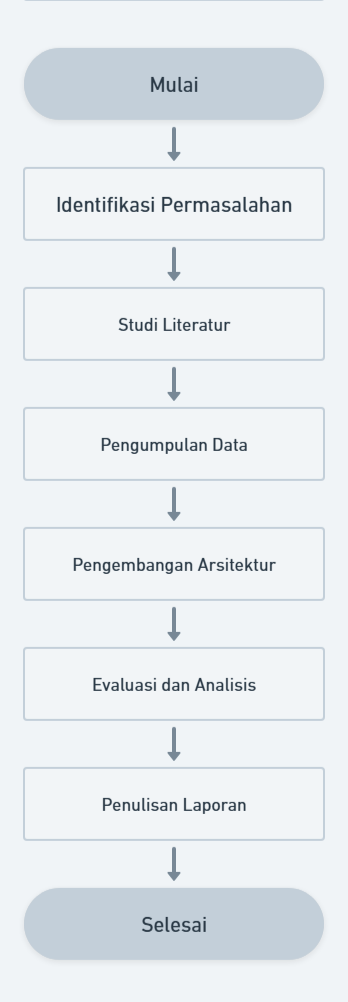
\includegraphics[width=0.3\textwidth]{images/alur-penelitian.png}
	\caption{
		Alur Penelitian
	}
	\label{fig:research-flow}
\end{figure}

Pelaksanaan penelitian ini akan mengikuti suatu alur yang terdiri dari beberapa tahapan utama yang saling terkait dan berurutan,
namun juga memungkinkan adanya iterasi pada beberapa fase tertentu, terutama pada tahap pengembangan dan evaluasi model.
Visualisasi alur penelitian ini disajikan dalam Gambar \ref{fig:research-flow}.
Tahapan-tahapan fundamental tersebut secara terperinci adalah sebagai berikut.


\subsection{Identifikasi Masalah}
Tahap awal ini merupakan fondasi dari keseluruhan penelitian. Proses ini dimulai dengan identifikasi masalah umum mengenai adanya kesenjangan akses terhadap informasi kesehatan mental yang akurat dan terstruktur di Indonesia.
Dari masalah umum tersebut, dirumuskan masalah teknis yang spesifik, yaitu bagaimana teknologi RAG dapat dioptimalkan untuk mengatasi tantangan ini.
Identifikasi masalah mencakup analisis kelemahan RAG berbasis potongan dokumen, yang cenderung kesulitan dalam melakukan penalaran atas hubungan kompleks.
Berdasarkan analisis ini, diajukan hipotesis bahwa penggunaan \textit{Knowledge Graph} dapat memberikan konteks yang lebih kaya dan terstruktur.
Tahapan ini menghasilkan rumusan masalah utama yang berfokus pada optimalisasi ekstraksi pengetahuan untuk membangun KG yang konsisten dan optimalisasi pengambilan pengetahuan dari KG untuk menjawab kueri pengguna secara akurat.

\subsection{Studi Literatur}
Studi literatur dilakukan secara sistematis, komprehensif, dan berkelanjutan.
Hal tersebut bertujuan membangun landasan teoritis yang kokoh, memahami tren dan perkembangan terkini \textit{state-of-the-art} dalam bidang terkait, mengidentifikasi celah penelitian (\textit{research gap}) yang dapat diisi, serta mempelajari berbagai metode dan alat bantu yang relevan.
Proses ini melibatkan pencarian, pengumpulan, analisis, dan sintesis informasi dari berbagai sumber ilmiah jurnal internasional seperti IEEE, ArXiv, JMIR, dll.
Fokus utama area studi literatur meliputi aplikasi teknologi AI pada kesehatan mental, RAG, dan \textit{Knowledge Graph}.
Setelah itu, dilakukan analisis mendalam mengenai metode \textit{Knowledge Extraction} dan \textit{Knowledge Retrieval} yang digunakan.

\subsection{Pengumpulan Data}
Pemilihan sumber data didasarkan pada serangkaian kriteria validasi yang telah ditetapkan demi menjaga kualitas sumber pengetahuan.
Kriteria ini bertujuan untuk menyaring informasi dan memastikan hanya konten yang berkualitas tinggi yang akan diintegrasikan ke dalam sistem.
Prinsip utama pemilihan data meliputi kredibilitas dan otoritas lembaga penyusun serta relevansinya terhadap isu kesehatan mental.
Sumber data harus berasal dari lembaga atau institusi yang memiliki otoritas dan rekam jejak yang diakui secara nasional dalam bidang kesehatan dan psikologi, seperti Kementerian Kesehatan, universitas, psikolog, dan lembaga lain.
Selain itu, konten yang terkandung harus relevan dengan permasalah kesehatan mental yang ada, berikut dengan fasilitas yang tersedia, pencegahan, edukasi, dsb.
Mengingat target implementasi sistem ini adalah untuk civitas akademika UGM, maka prioritas diberikan pada sumber data yang tidak hanya relevan untuk konteks kesehatan mental secara umum, tetapi juga spesifik dan dekat dengan lingkungan UGM.
Penggunaan sumber internal ini bertujuan untuk meningkatkan kepercayaan, kedekatan, dan relevansi informasi bagi pengguna akhir.

Berdasarkan kriteria yang ditetapkan, korpus data untuk penelitian ini dikumpulkan dari beberapa sumber, antara lain:

\begin{enumerate}
	\item \textbf{Kementerian Kesehatan (Kemenkes) RI}: Dokumen yang dipublikasikan oleh Kemenkes digunakan sebagai pedoman dasar yang berlaku secara nasional, memberikan pengetahuan mengengai kesehatan mental secara umum di Indonesia.
	\item \textbf{\textit{Center for Public Mental Health} (CPMH) Fakultas Psikologi UGM}: Sebagai pusat studi kesehatan mental, publikasi dari CPMH tidak hanya valid secara akademis, tetapi juga sangat relevan bagi civitas akademika UGM.
	\item \textbf{\textit{Health Promoting University} (HPU) UGM}: Materi dari HPU UGM dipilih karena secara spesifik dirancang untuk mempromosikan kesehatan di lingkungan kampus UGM. Informasi dari sumber ini, seperti mengenai layanan dukungan yang tersedia di UGM, akan sangat praktis dan langsung dapat dimanfaatkan oleh pengguna.
\end{enumerate}

Data yang terkumpul akan melalui proses kurasi untuk memastikan kesesuaian konten dan konsistensi informasi.
Setelah divalidasi, data kemudian akan melalui tahap prapemrosesan untuk membersihkan teks dan menyiapkannya untuk fase pengembangan arsitektur.

\subsection{Pengembangan Arsitektur Ekstraksi dan Penyerapan Pengetahuan}

\begin{figure}[H]
	\centering
	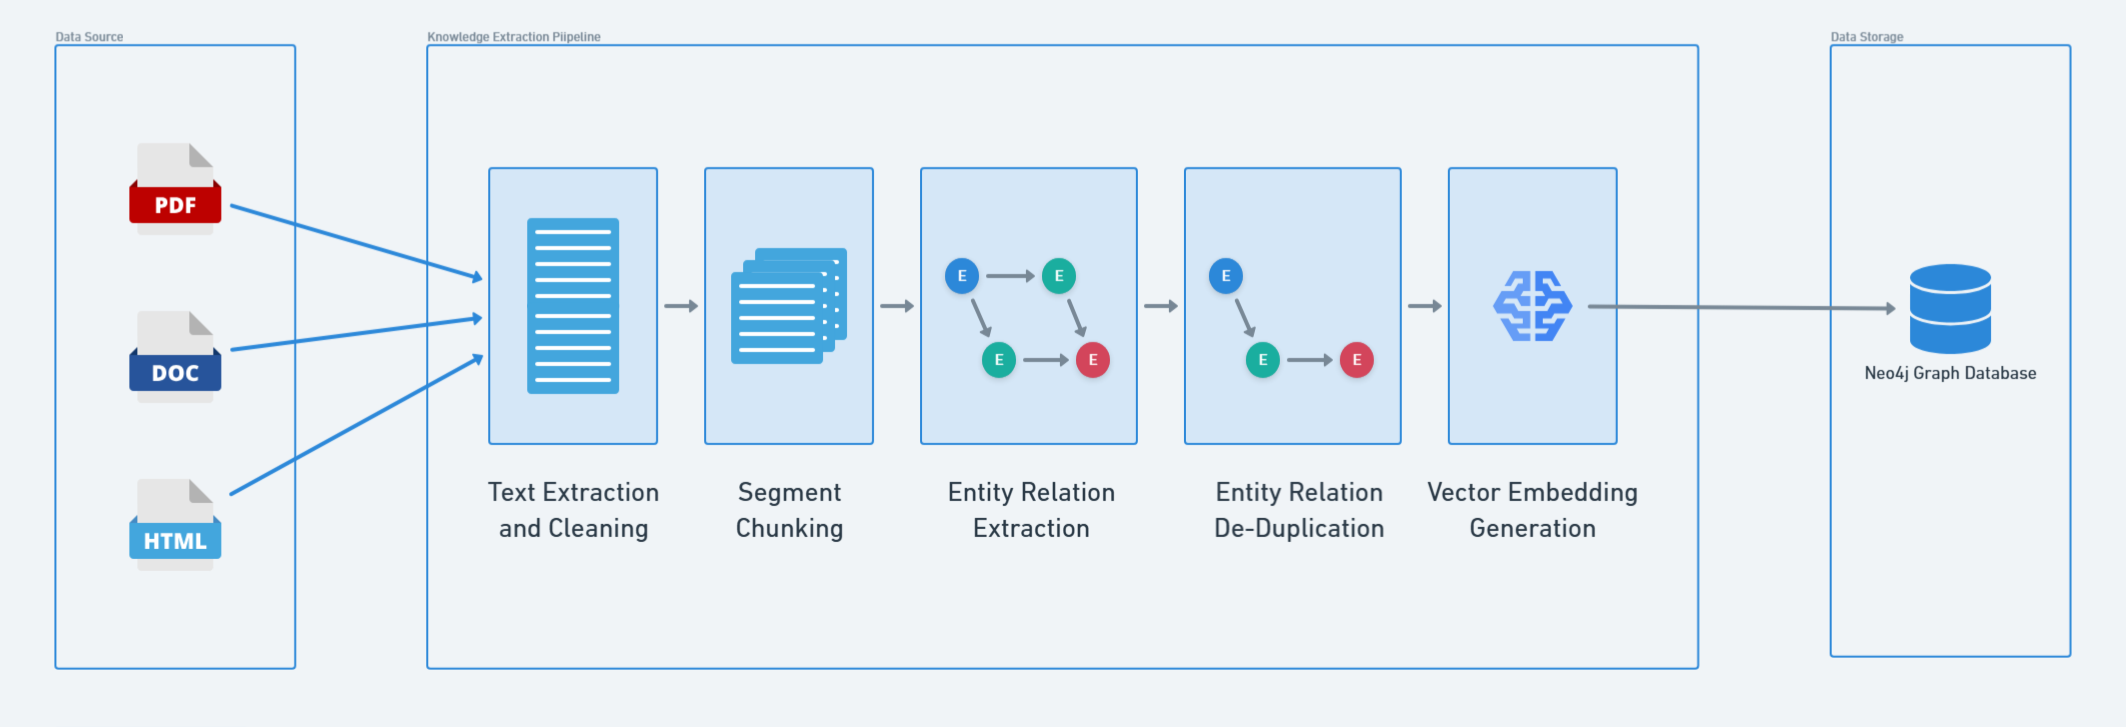
\includegraphics[width=1\textwidth]{images/knowledge-extraction-flow.png}
	\caption{
		\textit{Knowledge Extraction Pipeline}
	}
	\label{fig:knowledge-extraction-pipeline}
\end{figure}

Pengembangan model akan berfokus pada optimalisasi dua komponen krusial pada RAG berbasis \textit{Knowledge Graph}, yaitu \textit{Knowledge Extraction} dan \textit{Knowledge Retrieval}.
Tahap ini bertujuan untuk membangun \textit{Knowledge Graph} yang bersih, konsisten, dan kaya informasi dari berbagai sumber data yang mayoritas tidak terstruktur seperti PDF, DOCX, dan situs web.
Proses ekstraksi pengetahuan diimplementasikan melalui sebuah \textit{pipeline} seperti pada Gambar \ref{fig:knowledge-extraction-pipeline}.
Berikut merupakan penjelasan detail setiap langkah dalam \textit{pipeline}.

\subsubsection{Ekstraksi Teks dari Dokumen}
Hampir semua \textit{language model} dapat memahami informasi dalam bentuk teks.
Untuk itu, langkah awal membangun sebuah \textit{Knowledge Graph} adalah mengekstrak teks mentah dari berbagai sumber data.
Banyak data memiliki format, baik ekstensi, maupun struktur yang beragam karena berasal dari banyak sumber.
Setiap tipe dokumen memiliki cara mengekstraknya masing-masing, misalnya dokumen HTML dapat dikenali strukturnya melalui tagar HTML seperti \texttt{<h1>} untuk menyatakan judul dan \texttt{<p>} untuk menyatakan paragraf.
Dokumen bertipe DOCX terdiri dari kumpulan \textit{file} ZIP yang harus diekstrak untuk mengambil isi dokumen.
Setiap dokumen tersebut juga memiliki struktur penulisan yang tidak seragam, seperti pada dokumen HTML belum tentu mengandung tagar \textit{headline} (\texttt{<h1>}, \texttt{<h2>}, sampai \texttt{<h6>}) untuk menulis, melainkan memakai tagar \texttt{<div>}.
Ketakseragaman format tersebut menjadi tantangan tersendiri dalam mengekstrak teks dari dokumen yang beragam.

Dokumen yang digunakan dalam membangun KG meliputi.
\begin{enumerate}
	\item Buku "Petunjuk Teknis Pencegahan dan Pengendalian Gangguan Mental Emosional" dari Kementerian Kesehatan.
	\item Buku "Panduan Kesehatan Jiwa pada Masa Pandemi COVID-19" dari Kementerian Kesehatan.
	\item Buku "Panduan Pertolongan Pertama Psikologis Pada Upaya Bunuh Diri" dari CPMH.
	\item Artikel dari situs web CPMH
	\item Artikel dari situs web HPU UGM
\end{enumerate}

Sebagian besar dokumen tersebut berada dalam format PDF, sedangkan artikel dari situs web CPMH dan HPU UGM berada dalam format HTML.
Mengekstrak \textit{file} PDF dengan mempertahankan struktur dokumen cukup sulit untuk dilakukan secara langsung karena PDF merupakan tipe dokumen berbasis halaman (\textit{page}) yang mengabaikan struktur keseluruhan seperti judul, paragraf, atau tabel.
Informasi mengenai struktur dokumen penting dijaga untuk langkah selanjutnya.
Untuk itu, dilakukan strategi konversi \textit{file} PDF ke dalam bentuk dokumen yang lebih terstruktur seperti DOCX dan HTML.
Konversi dilakukan menggunakan layanan konversi file online \href{https://www.freeconvert.com/}{FreeConvert}.
Setelah dilakukan konversi dokumen PDF menjadi DOCX barulah isi dari dokumen dapat diambil.
Ekstraksi teks mentah dari dokumen dilakukan menggunakan pustaka python-docx dengan mengambil semua teks yang ada beserta dengan tabel.
Sementara itu, dokumen artikel dari situs web CPMH dan HPU UGM berformat HTML, sehingga proses ekstraksinya lebih sederhana.
Ekstraksi dari HTML lebih mudah karena format ini sudah memiliki struktur bawaan melalui penggunaan tag.
Misalnya, tag \texttt{<h1>} digunakan untuk judul, \texttt{<p>} untuk paragraf, dan \texttt{<table>} untuk tabel.
Untuk merepresentasikan tabel dalam bentuk teks mentah, digunakan format tabel markdown yang intuitif dan mudah dipahami oleh sebagian besar LLM.

\subsubsection{\textit{Structural Chunking}}
Teks yang diekstrak dari dokumen pada langkah selanjutnya akan diekstrak lagi entitas dan relasi yang terkandung di dalamnya.
Ekstraksi entitas dan relasi dilakukan dengan menggunakan LLM.
Namun, LLM modern memiliki ukuran \textit{context window} yang terbatas berkisar ratusan ribu (GPT 4o) hingga 10 juta token (Meta Llama 4 Scout).
Keterbatasan tersebut berimplikasi pada ukuran dokumen (dalam satuan token) menjadi hal yang perlu diperhatikan mengingat sebuah dokumen dapat memiliki ukuran yang besar.
Analisis menggunakan LLM dengan dokumen yang melebihi atau mendekati ukuran maksimal \textit{context window} tidak akan maksimal karena LLM gagal memahami konteks dokumen secara keseluruhan.
Untuk itu, dokumen perlu dipecah menjadi beberapa bagian yang disebut \textit{chunk}.

Proses \textit{chunking} secara umum dapat dilakukan dengan memecah dokumen menjadi beberapa \textit{chunk} dengan panjang tertentu.
Metode \textit{chunking} seperti itu cukup mudah dilakukan, tetapi ada potensi bagian kata atau kalimat dapat terpisah antar \textit{chunk} akibat pemotongan yang menyebabkan kehilangan makna dan konteks.
Dokumen yang masih memiliki informasi strukturnya dapat dimanfaatkan untuk melakukan pemecahan dokumen.
Alih-alih memotong dokumen menjadi potongan berukuran tetap, dokumen dibagi berdasarkan format struktural tertentu, misal dalam dokumen HTML berupa tag \texttt{<h1>} atau pada dokumen DOCX berupa \textit{style paragraph heading} atau \textit{title}.
Pada buku "Petunjuk Teknis Pencegahan dan Pengendalian Gangguan Mental Emosional" yang telah dikonversi menjadi DOCX, dipecah menjadi beberapa chunk berdasarkan judul-judul bagian (seperti BAB I, BAB II, dst).
Pemecahan dokumen berdasarkan judul bagian menghasilkan pecahan dokumen yang memiliki konteks utuh karena pada umumnya setiap bagian dalam dokumen menjelaskan suatu topik bahasan secara utuh.
Hasil dari pemecahan dokumen tersebut yang berjumlah 13 \textit{chunk} kemudian disimpan dalam format TXT untuk kebutuhan \textit{tracing}.
Untuk dokumen yang tidak terlampau panjang tidak akan dipecah, tetapi langsung menjadi 1 bagian dokumen utuh.

\subsubsection{Ekstraksi Entitas dan Relasi}
Ekstraksi entitas dan relasi dalam penelitian ini dilakukan melalui mekanisme inferensi dokumen menggunakan LLM.
Penggunaan LLM untuk mengekstrak entitas dan relasi didasarkan pada kemampuannya dalam memahami struktur dan konteks dokumen yang kompleks dan berukuran besar berkat arsitekturnya yang dilengkapi dengan jumlah parameter yang sangat besar hingga triliunan parameter.
Kapasitas ini memungkinkan LLM untuk menangkap pola linguistik, semantik, dan hubungan antar entitas secara lebih mendalam.
LLM yang digunakan sebagai basis ekstraksi entitas dan relasi adalah Google Gemini 2.5 Flash.
Pemilihan model tersebut didasarkan pada performanya yang sangat baik dan masuk dalam \textit{leaderboard} paling atas pada \href{https://llm-stats.com/}{LLM Stats} setidaknya saat penelitian ini dilakukan dengan skor GPQA (\textit{Graduate-Level Google-Proof Question and Answer}) sebesar 82,8\%.
Faktor krusial lainnya yang tidak kalah penting adalah Gemini 2.5 Flash memiliki ukuran \textit{context window} yang sangat besar hingga 1 juta dibandingkan model LLM lain seperti Claude 3.7 Sonet, Grok-3, dan GPT o3.
Perbandingan performa dan kapasitas LLM tersebut dapat dilihat pada Tabel \ref{tab:llm-comparison}.

\begin{table}[ht]
	\centering
	\caption{Perbandingan performa dan kapasitas LLM modern}
	\label{tab:llm-comparison}
	\begin{tabular}{|l|c|c|}
		\hline
		\textbf{Model}   & \textbf{GPQA} & \textbf{\textit{Context Window}} \\
		\hline \hline
		Gemini 2.5 Flash & 82,8\%        & 1.048.576                        \\
		\hline
		Claude Sonnet 4  & 83,8\%        & 200.000                          \\
		\hline
		OpenAI o3        & 83,3\%        & 200.000                          \\
		\hline
		Grok-3           & 84,6\%        & 128.000                          \\
		\hline
	\end{tabular}
\end{table}

\pagebreak
Setiap \textit{chunk} teks dari dokumen kemudian diproses oleh Gemini 2.5 Flash untuk mengekstrak entitas dan relasi yang terkandung di dalamnya.
Proses ini memanfaatkan teknik \textit{few-shot prompting}, di mana LLM diberikan beberapa contoh konkret untuk memandunya dalam melakukan ekstraksi sesuai dengan ontologi yang telah didefinisikan.
\textit{Prompt} dirancang sejelas mungkin untuk menjelaskan apa yang seharusnya dilakukan oleh LLM dalam proses ekstraksi.
Untuk menjaga jenis entitas yang ditemukan dalam dokumen tidak keluar dari tujuan layanan kesehatan mental maka beberapa istilah yang berkaitan telah didefinisikan terlebih dahulu dalam \textit{prompt}.
Format respons dari LLM juga didefinisikan berupa tipe data JSON yang memudahkan dalam pemrosesan selanjutnya. Format instruksi \textit{prompt} dapat dilihat pada Gambar \ref{fig:prompt-extraction-instruction}.

\begin{figure}[H]
	\centering
	\fbox{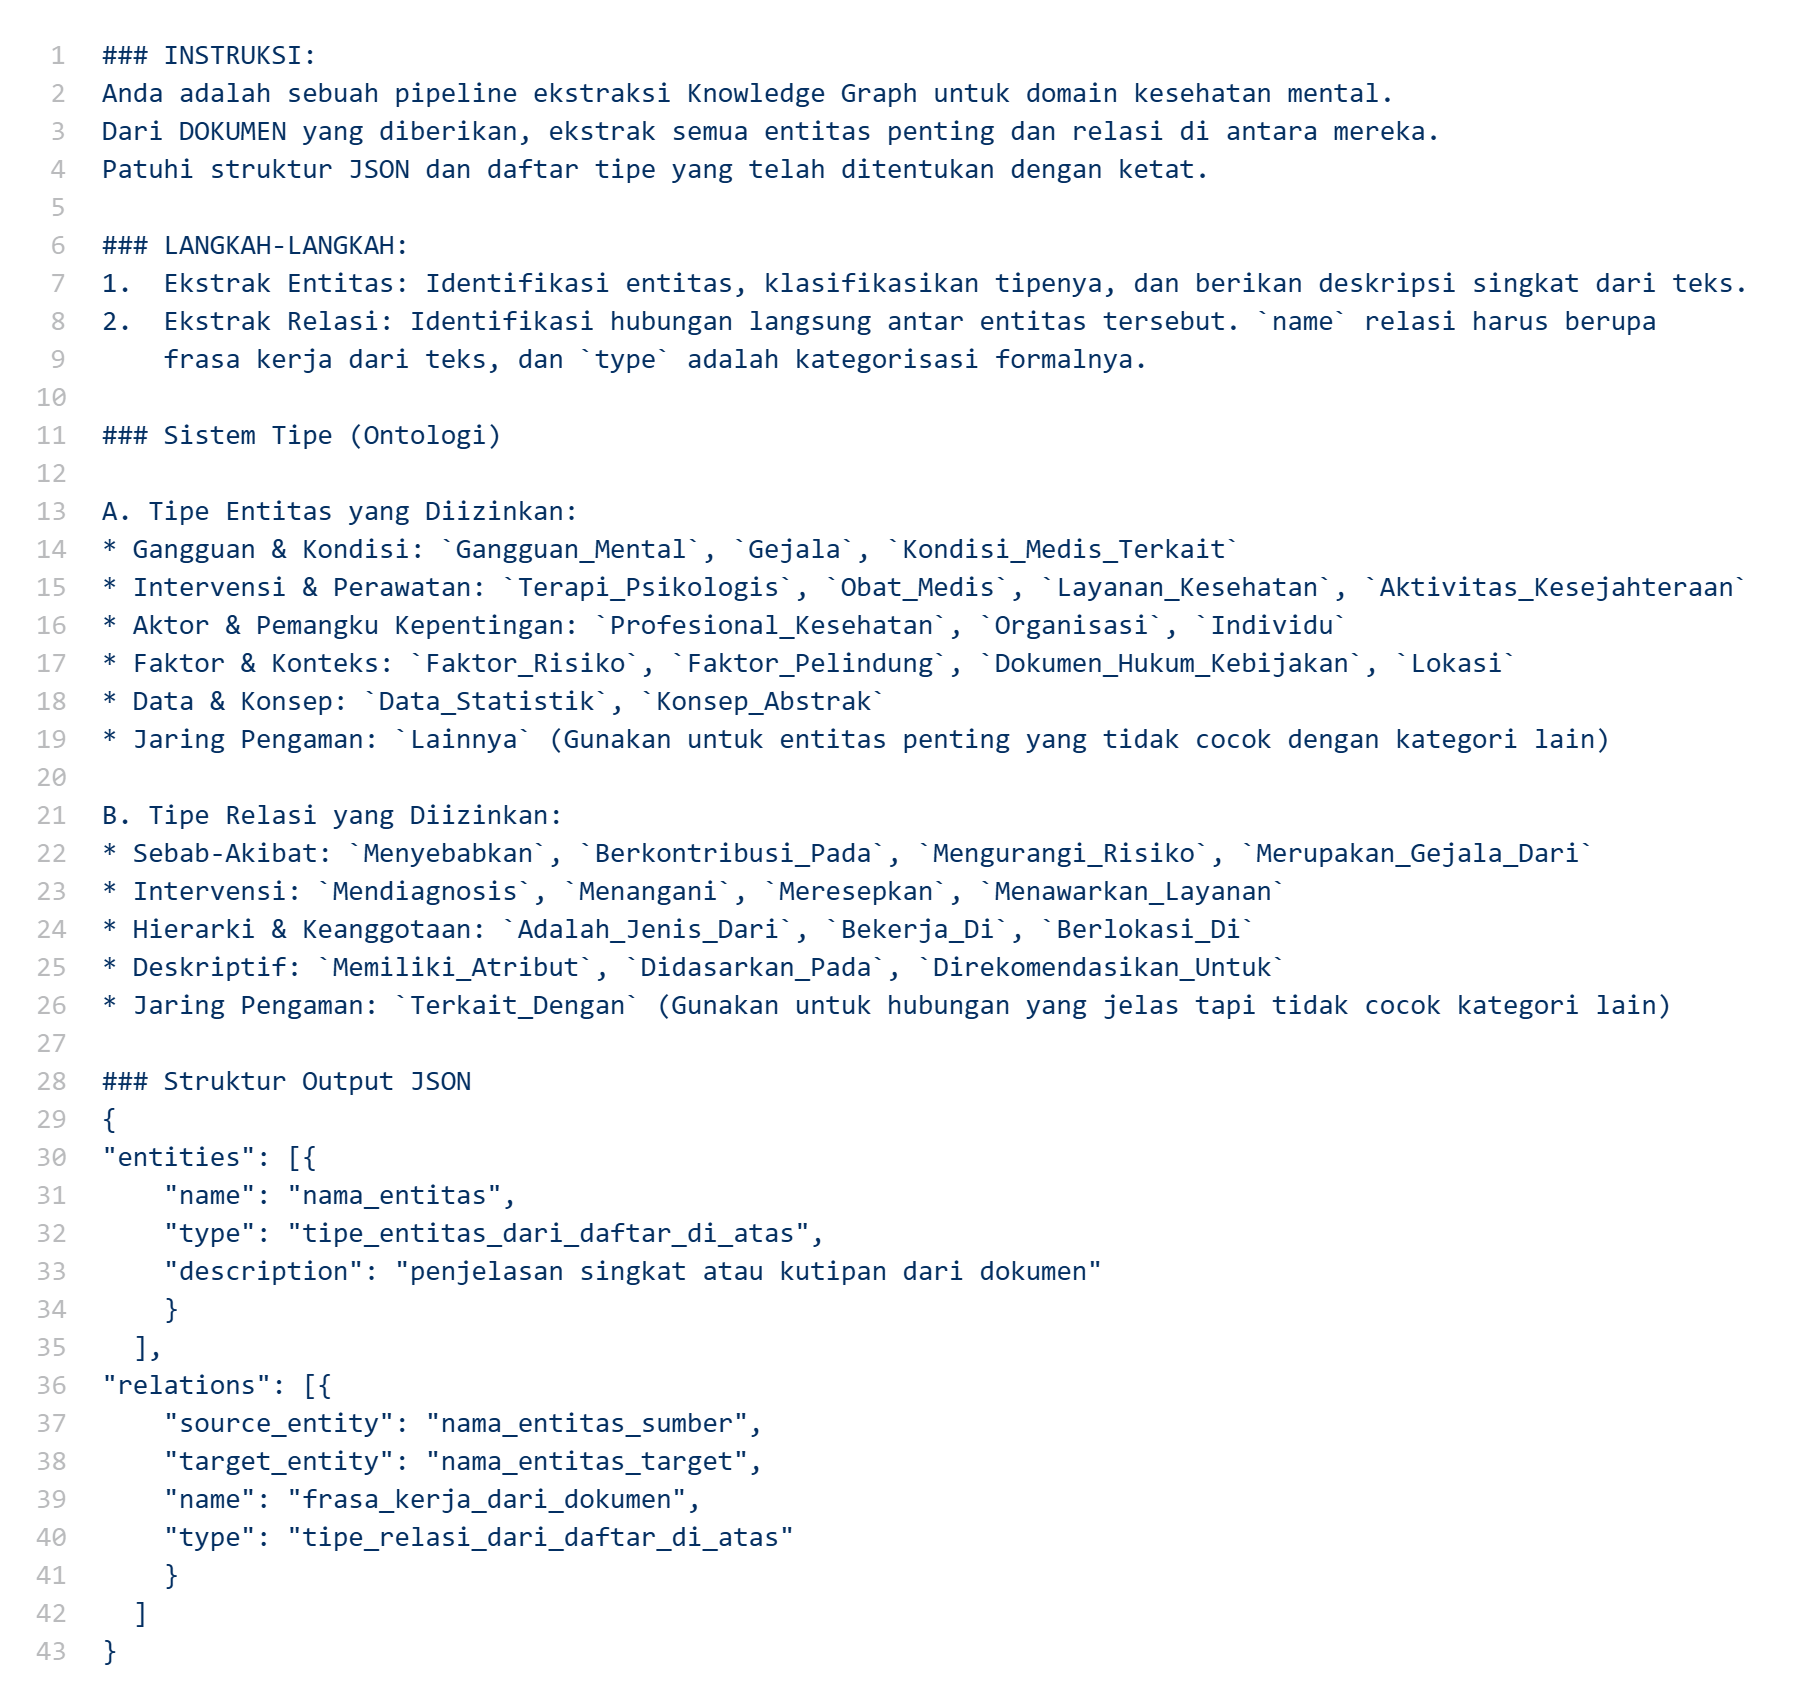
\includegraphics[width=1\textwidth]{images/prompt-extraction-instruction.png}}
	\caption{
		Instruksi LLM untuk melakukan ekstraksi entitas dan relasi
	}
	\label{fig:prompt-extraction-instruction}
\end{figure}

Selain pembatasan istilah dan pemberian instruksi, teknik \textit{few-shot prompting} juga digunakan untuk menghasilkan respons sesuai dengan apa yang diinginkan.
\textit{Few-shot prompting} telah teruji memberikan peningkatan yang signifikan terhadap performa LLM dibandingkan dengan \textit{zero-shot prompting} yang hanya memberikan instruksi saja tanpa contoh \cite{LLMisFewShot2020}.
Teknik ini dilakukan dengan memberikan beberapa contoh (\textit{shot}) input yang akan dihadapi beserta respons yang diharapkan.
Sebuah potongan dari dokumen ditambahkan sebagai contoh input dokumen yang akan diekstrak diikuti dengan keluaran yang diharapkan menggunakan format JSON.
Contoh masukkan dan keluaran pada \textit{prompt} dapat dilihat pada Gambar \ref{fig:prompt-extraction-few-shot}.

\begin{figure}[H]
	\centering
	\fbox{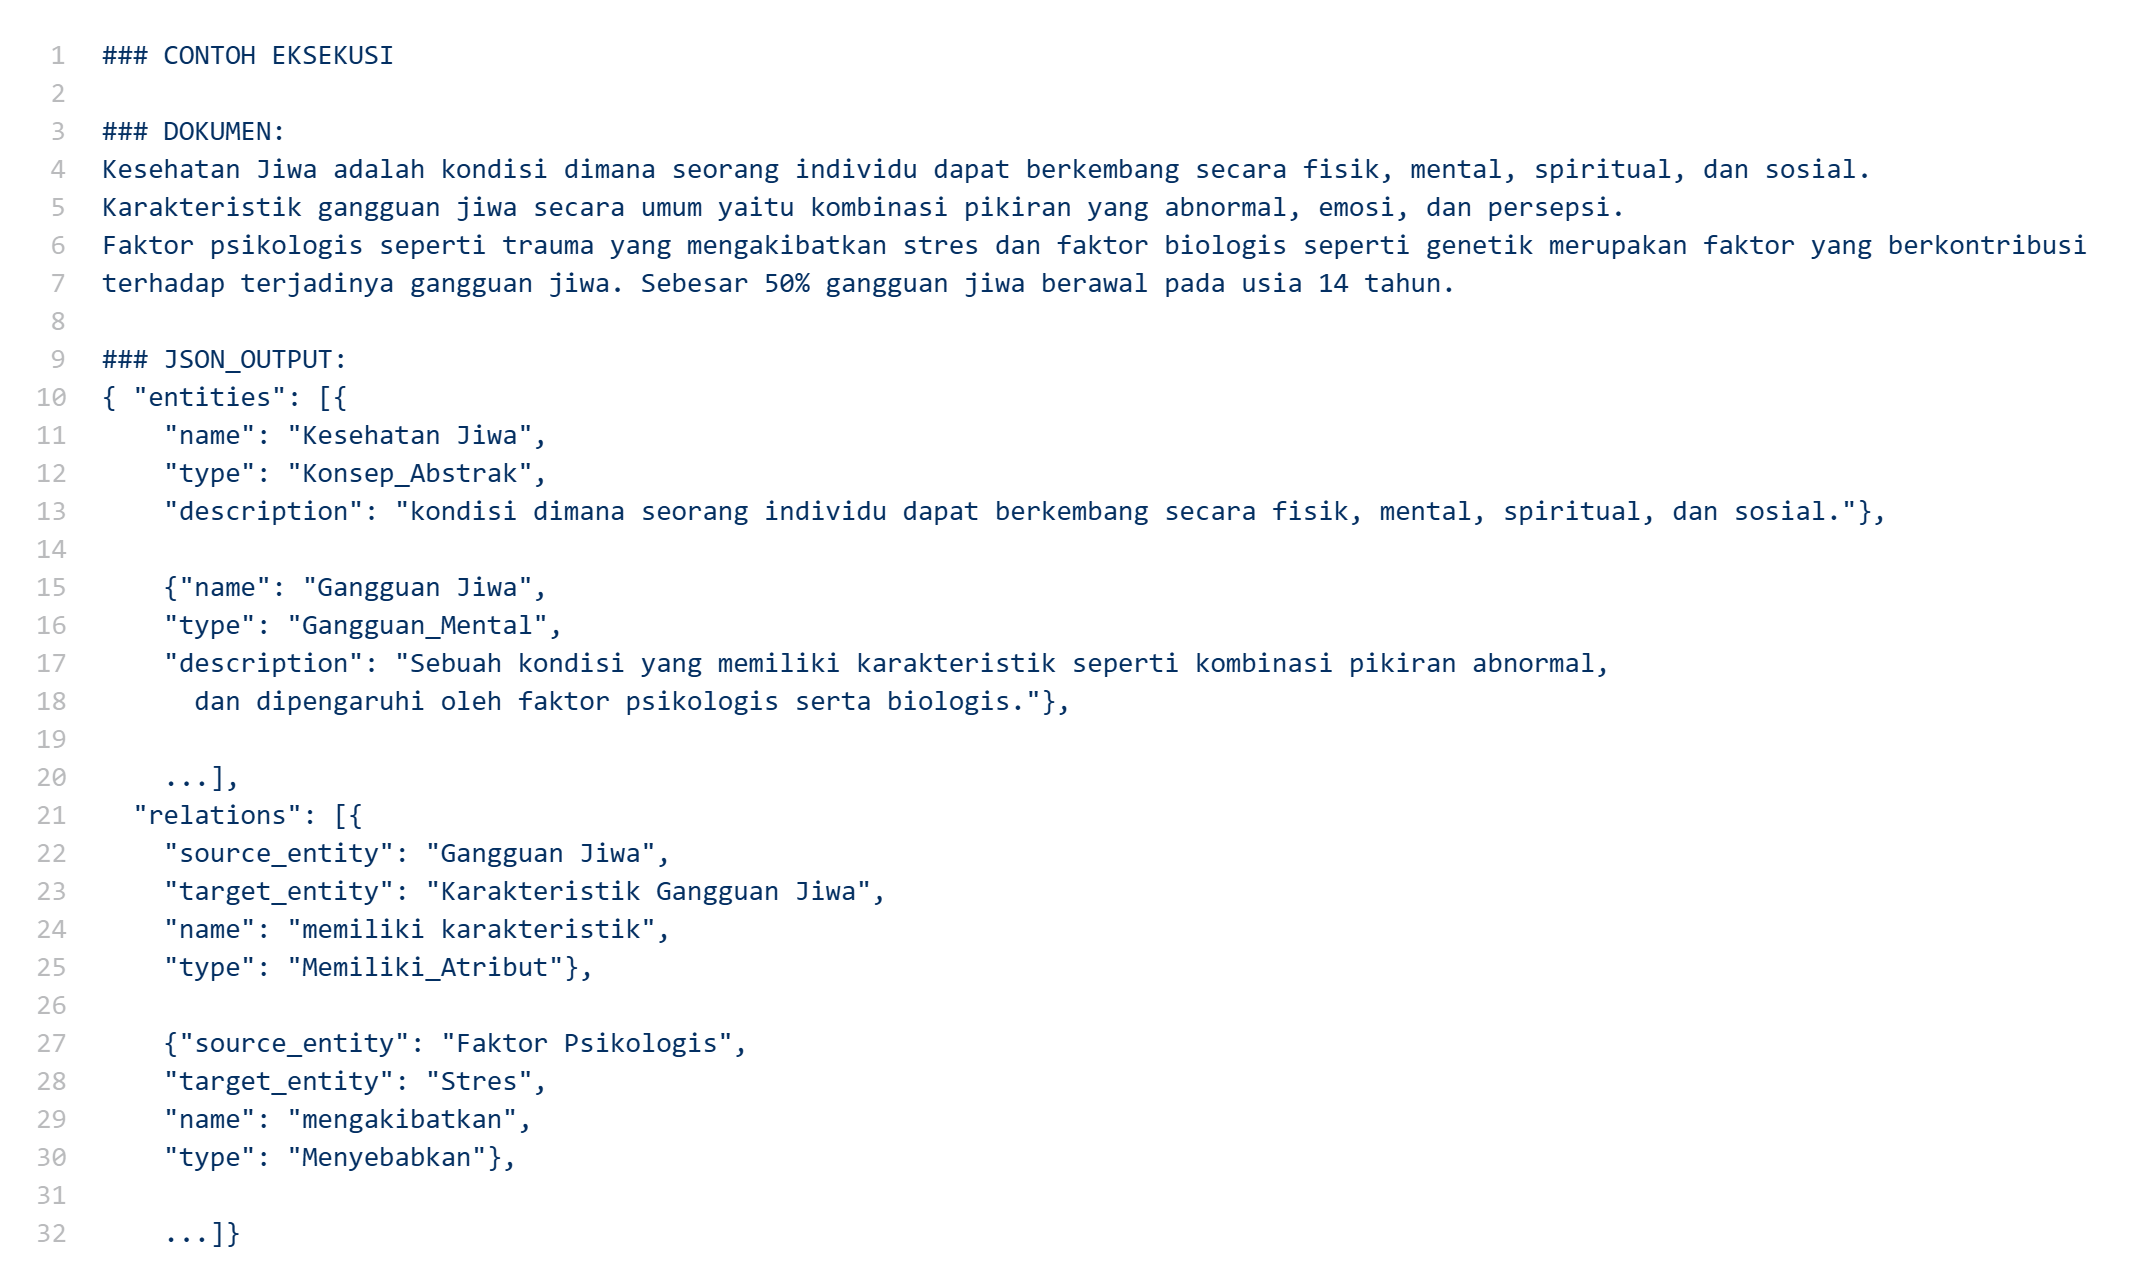
\includegraphics[width=1\textwidth]{images/prompt-extraction-few-shot.png}}
	\caption{
		Penggunaan \textit{few-shot prompting} dengan memberikan potongan dokumen dan keluaran yang diharapkan.
	}
	\label{fig:prompt-extraction-few-shot}
\end{figure}

% \vspace{5cm}
\textit{Prompt} pada Gambar \ref{fig:prompt-extraction-instruction} dan Gambar \ref{fig:prompt-extraction-few-shot} kemudian dieksekusi menggunakan pustaka google genai.
Eksekusi \textit{prompt} diikuti dengan data \textit{chunk} dokumen ditambah dengan konfigurasi struktur JSON yang diinginkan untuk mendapatkan respons bukan dalam bentuk teks, melainkan dalam bentuk JSON yang dapat direpresentasikan dalam bentuk objek pydantic.
Struktur dari respons terbagi menjadi 2 bagian yaitu \texttt{entities} yang berisi daftar entitas dan \texttt{relations} yang berisi daftar relasi.
Setiap entitas memiliki atribut \texttt{name}, \texttt{type}, dan \texttt{description}, sedangkan relasi memiliki atribut \\
\texttt{source\_entity}, \texttt{target\_entity}, \texttt{name}, dan \texttt{type} seperti pada Gambar \ref{fig:entity-relation-structure}.

\begin{figure}[H]
	\centering
	\fbox{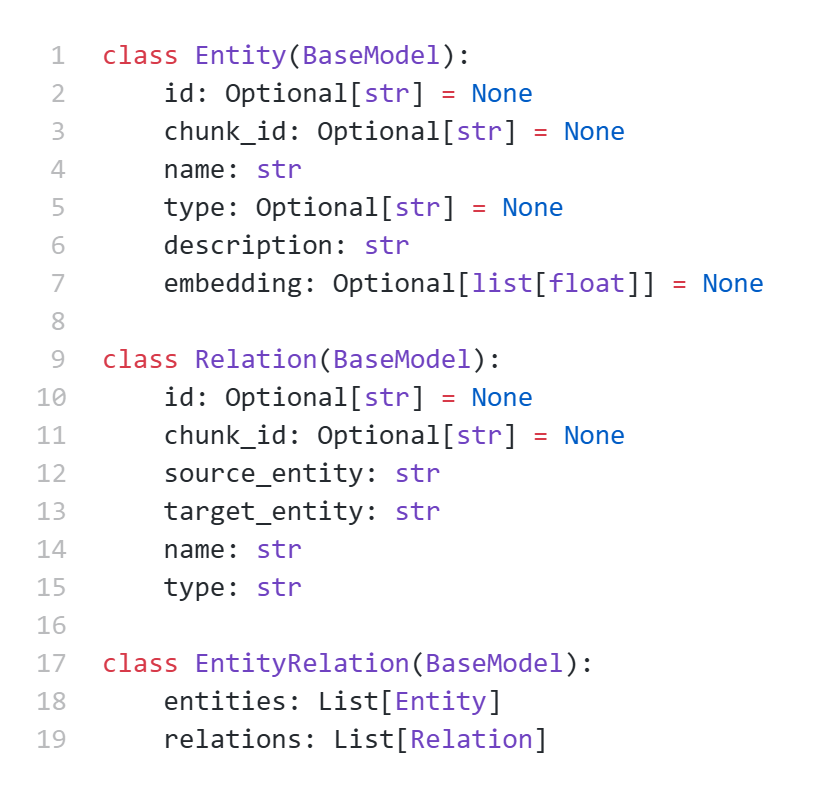
\includegraphics[width=0.5\textwidth]{images/entity-relation-structure.png}}
	\caption{
		Struktur entitas dan relasi yang didefinisikan sebagai \textit{objek} pada pustaka Pydantic
	}
	\label{fig:entity-relation-structure}
\end{figure}

Hasil dari eksekusi \textit{prompt} menghasilkan kumpulan entitas dan relasi dengan format persis seperti skema yang didefinisikan sebelumnya.
Gambar \ref{fig:entity-relation-response} menunjukkan entitas dan relasi yang diekstrak dari potongan dokumen pada Gambar \ref{fig:document-mini-chunk-example}.
\begin{figure}[H]
	\centering
	\fbox{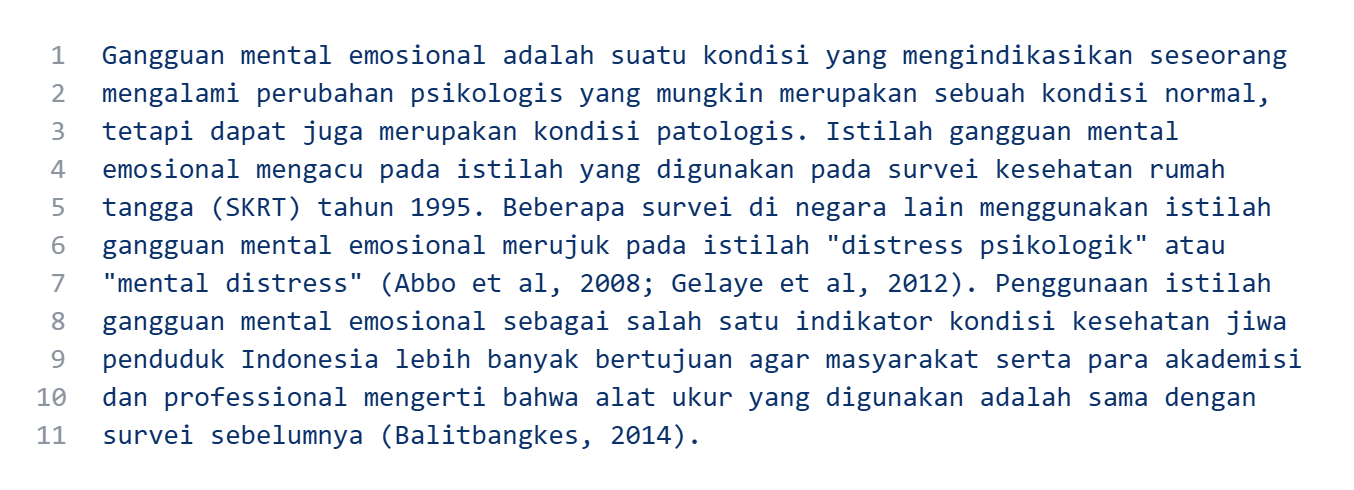
\includegraphics[width=1\textwidth]{images/document-mini-chunk-example.png}}
	\caption{
		Cuplikan dokumen yang diambil dari Buku Petunjuk Teknis Pencegahan dan Pengendalian Gangguan Mental Emosional
	}
	\label{fig:document-mini-chunk-example}
\end{figure}

\begin{figure}[H]
	\centering
	\fbox{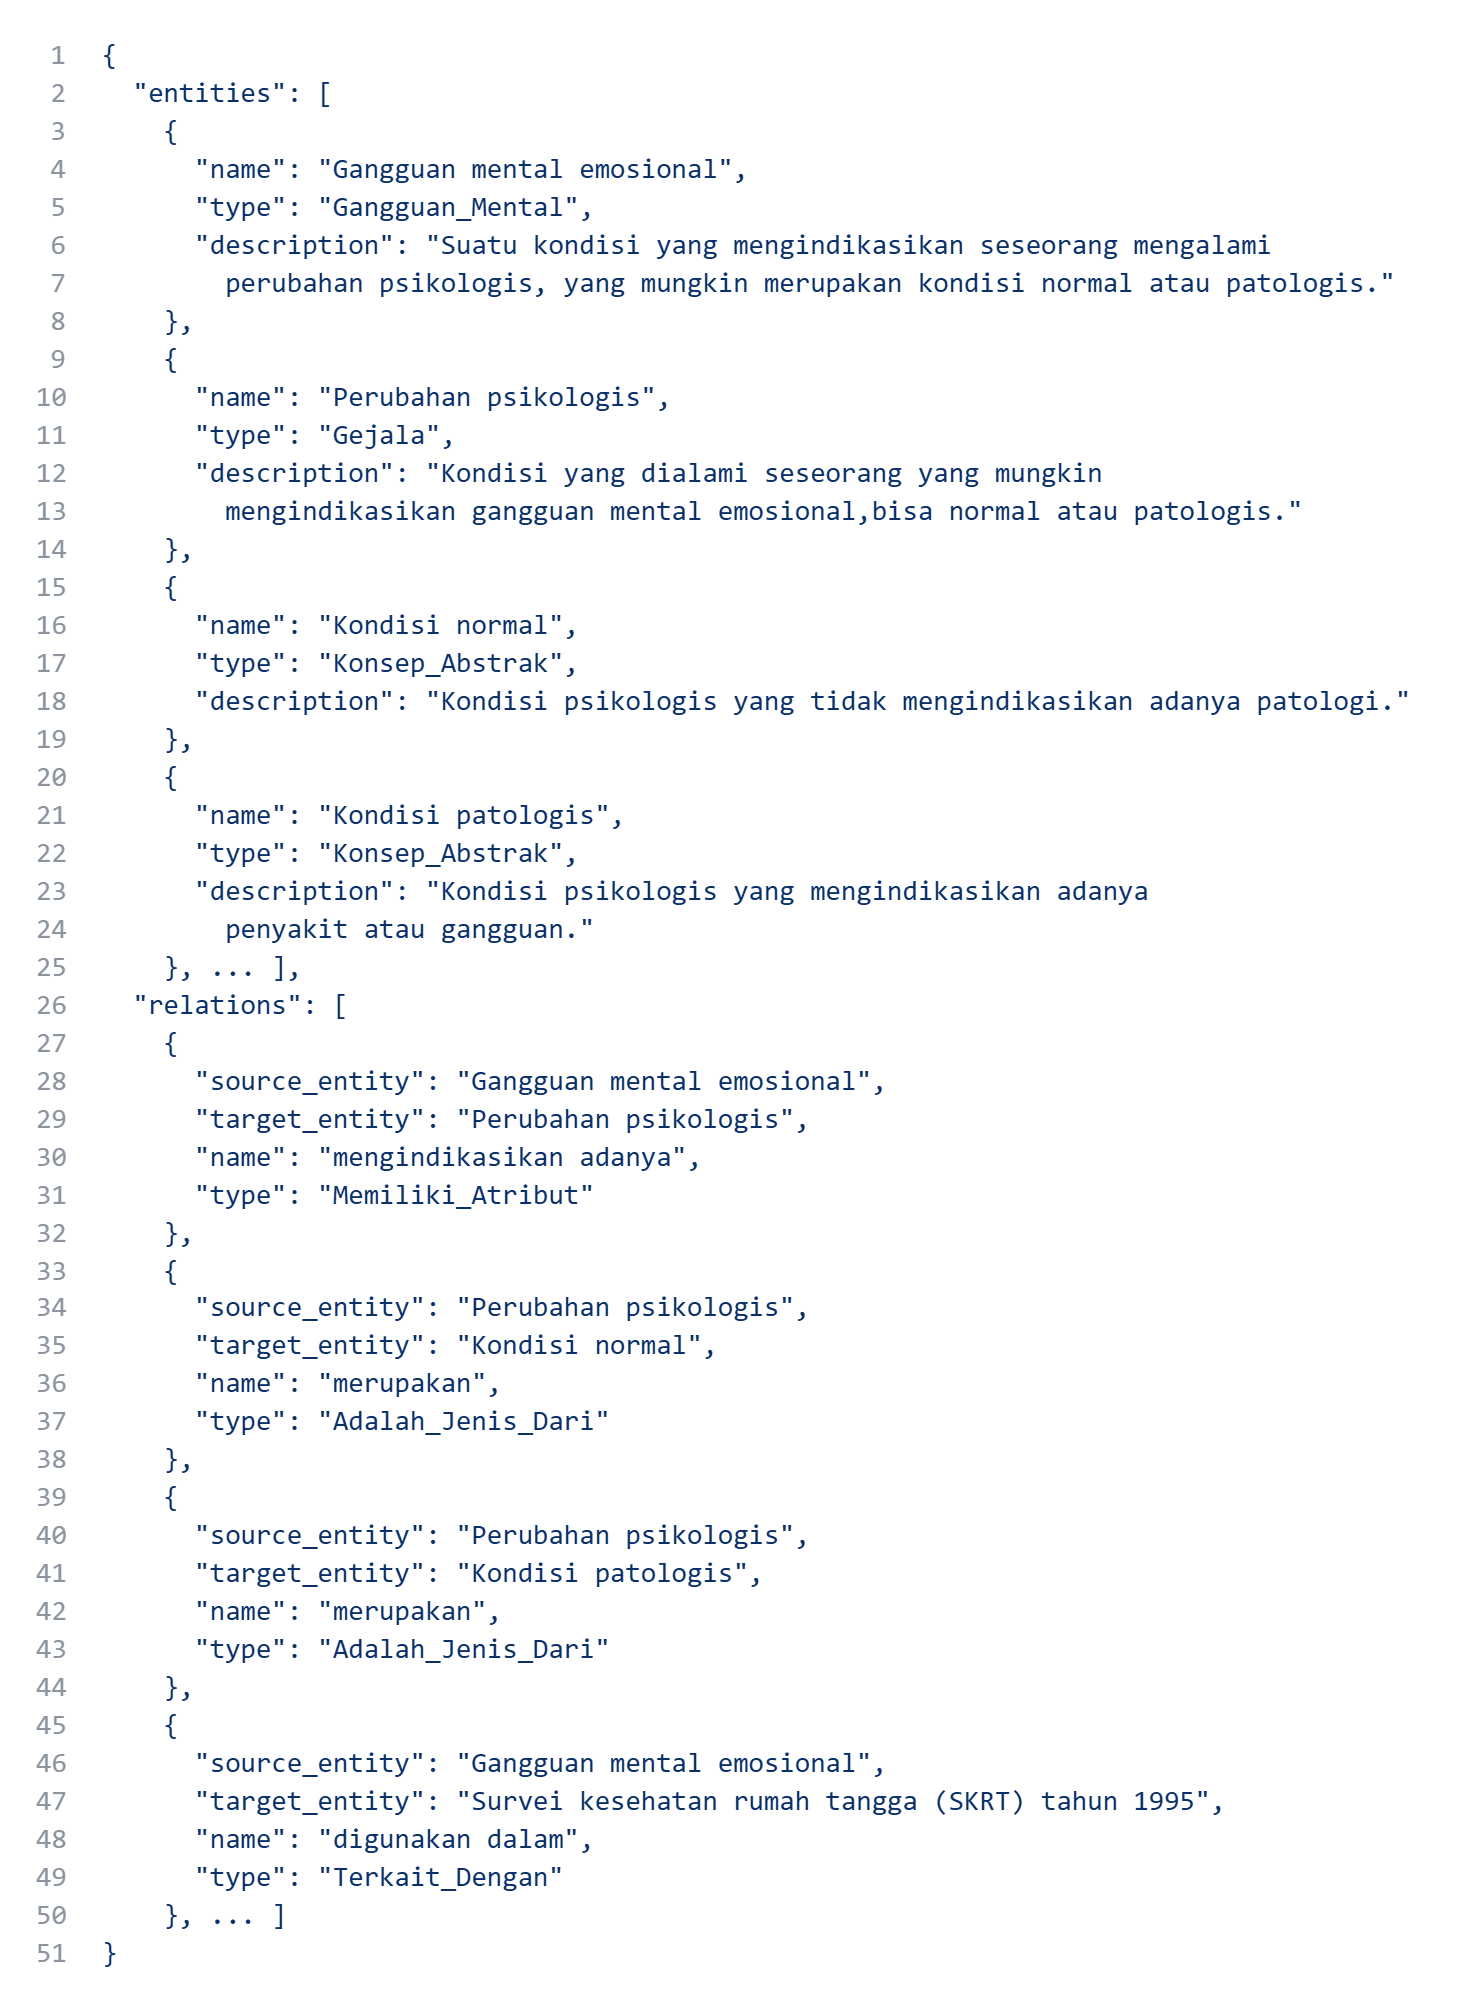
\includegraphics[width=0.8\textwidth]{images/entity-relation-response.png}}
	\caption{
		Respons LLM berupa entitas dan relasi yang diekstrak dari potongan dokumen
	}
	\label{fig:entity-relation-response}
\end{figure}

\subsubsection{Resolusi Entitas dan Relasi}

Hasil dari entitas dan relasi yang telah berhasil diekstrak dari setiap \textit{chunk} kemudian diagregasi dan melalui tahap resolusi untuk memastikan konsistensi.
Entitas dan relasi yang berasal dari \textit{chunk} berbeda mungkin akan memiliki duplikat karena diekstrak secara independen.
Untuk itu, perlu untuk melakukan deduplikasi pada entitas dan relasi guna menghindari redudansi yang tidak perlu.
Entitas yang redundan dapat membuat graf semakin kompleks dan merusak mekanisme \textit{retrieval}.
Deduplikasi dilakukan dengan strategi penggabungan di mana entitas yang memiliki nama yang sama setelah dinormalisasi akan digabungkan menjadi satu.
Untuk mengatasi kehilangan informasi maka deskripsi unik dari entitas duplikat kemudian digabungkan menjadi satu deskripsi utuh.
\textit{Entity mapping} dibentuk saat proses deduplikasi entitas untuk memetakan \texttt{source\_entity} dan \texttt{target\_entity} pada relasi ke entitas yang valid.

\subsubsection{Penambahan Vektor \textit{Embedding}}

Data entitas dan relasi yang disimpan dalam basis data secara umum adalah kumpulan teks yang cukup intuitif bagi manusia untuk memahaminya.
Meskipun demikian, komputer tidak dapat secara langsung "memahami" makna dari tiap-tiap entitas dan relasi.
Bagi manusia mungkin akan mudah untuk mencari entitas dengan nama atau deskripsi yang berkaitan dengan kata kunci atau pertanyaan pengguna.
Untuk itu, diperlukan sebuah representasi tertentu dari data yang dapat dengan mudah dipahami maknanya oleh komputer.
Salah satu representasi data yang cukup mudah diolah oleh komputer sekaligus dapat menangkap makna semantik dari data adalah vektor \textit{embedding}.
Vektor \textit{embedding} merupakan sebuah vektor berdimensi tinggi yang umum digunakan untuk menangkap makna dari sebuah data.
Data dalam bentuk vektor memiliki keuntungan dalam melakukan pencarian semantik (\textit{semantic search}) dengan hanya melakukan operasi \textit{dot product} 2 vektor dapat mengetahui tingkat kemiripan antara 2 data.

Dalam penelitian ini, objek yang akan dilakukan pencarian semantik dalam prosen \textit{knowledge retrieval} adalah entitas.
Untuk itu, setiap entitas akan memiliki representasi vektornya masing-masing.
Vektor \textit{embedding} akan dibentuk menggunakan model gemini-embedding-001.
Model \textit{embedding} ini dipilih menjadi model \textit{embedding} karena memiliki performa yang sangat baik dalam tugas \textit{Semantic Text Similarity} (STS) sebesar 79,40 poin.
Selain itu, model ini juga memiliki kemampuan memahami teks dalam bahasa Indonesia paling baik (67,00 poin) dibandingkan dengan model-model lain \cite{enevoldsen2025MMTEBmassivemultilingualtextEmbeddingModelComp}.
Perbandingan model \textit{embedding} dapat dilihat pada Tabel \ref{tab:embedding-model-comparison}.

\begin{table}[h]
	\centering
	\caption{Perbandingan model \textit{embedding} dalam tugas \textit{Semantic Text Similarity} (STS) dan klasifikasi dalam bahasa Indonesia \cite{enevoldsen2025MMTEBmassivemultilingualtextEmbeddingModelComp}}
	\label{tab:embedding-model-comparison}
	\begin{tabular}{|l|c|c|}
		\hline
		\textbf{Model}       & \textbf{IndoneisanIdClickbaitClassification} & \textbf{{STS}} \\
		\hline \hline
		gemini-embedding-001 & 67,00                                        & 79,40          \\
		\hline
		Qwen3-Embedding-8B   & 65,07                                        & 81.08          \\
		\hline
		Qwen3-Embedding-0,6B & 64,77                                        & 76,17          \\
		\hline
		Qwen3-Embedding-4B   & 64,29                                        & 80,86          \\
		\hline
		voyage-multiligual-2 & 63,23                                        & 68,58          \\
		\hline
	\end{tabular}
\end{table}

Data yang digunakan untuk membuat vektor \textit{embedding} berasal dari gabungan nama, tipe, dan deskripsi dari setiap entitas.
Proses pembuatannya dilakukan secara berulang dengan 100 entitas setiap satu kali pemanggilan API gemini-embedding-001.
Pemanggilan tersebut menghasilkan sebuah vektor dengan 768 dimensi untuk setiap entitas.
Hasil yang berupa vektor tersebut kemudian digabungkan dengan entitas yang bersesuaian dengan atribut \texttt{embedding}.

\subsubsection{Pemuatan Data ke Penyimpanan Basis Data Berbasis Graf}
Entitas dan relasi yang telah dilengkapi dengan vektor \textit{embedding} kemudian dimuat ke dalam basis data graf.
Basis data graf yang dipilih adalah Neo4j karena kemampuannya dalam menyimpan dan menavigasi struktur relasi antar entitas secara efisien, serta mendukung kueri berbasis graf melalui bahasa Cypher.
Neo4j juga mendukung algoritma pencarian berbasis vektor seperti \textit{Approximate Nearest Neighbor} (ANN) secara \textit{native} dengan menerapkan algoritma \textit{Hierarchical Navigable Small World} (HNSW).
Dukungan ini menjadi krusial untuk memungkinkan pencarian semantik dijalankan secara optimal.
Selain itu, Neo4j merupakan sistem basis data yang telah matang dan banyak digunakan, sehingga memiliki dukungan komunitas yang kuat. Dalam pemodelan data, setiap entitas direpresentasikan sebagai \textit{node} dengan atribut seperti \texttt{name}, \texttt{type}, dan \texttt{embedding}, sementara relasi dimodelkan sebagai \textit{edge} yang menghubungkan dua \textit{nodes} dan memiliki atribut seperti \texttt{source\_entity}, \texttt{target\_entity}, \texttt{name}, dan \texttt{type}.
Proses pemuatan data ke Neo4j dilakukan dengan melakukan inisialisasi koneksi ke server, lalu menyusun kueri untuk menambahkan \textit{node} dan \textit{edge} sesuai skema.
Untuk menghindari duplikasi \textit{node}, digunakan pendekatan \texttt{MERGE} dalam Cypher, sehingga entitas dengan identitas yang sama tidak dibuat ulang seperti pada Gambar \ref{fig:cypher-insert-entities}.
Proses ini juga mempertimbangkan efisiensi, khususnya ketika jumlah entitas dan relasi sangat besar, dengan menerapkan strategi \textit{batch insert}.
Dengan memanfaatkan basis data graf, relasi antar entitas dapat ditelusuri secara lebih fleksibel dan intuitif.
Hal ini juga mendukung berbagai analisis struktur data seperti pencarian pola hubungan, pengukuran kedekatan antar \textit{node}, hingga identifikasi komunitas dalam graf.

\begin{figure}[H]
	\centering
	\fbox{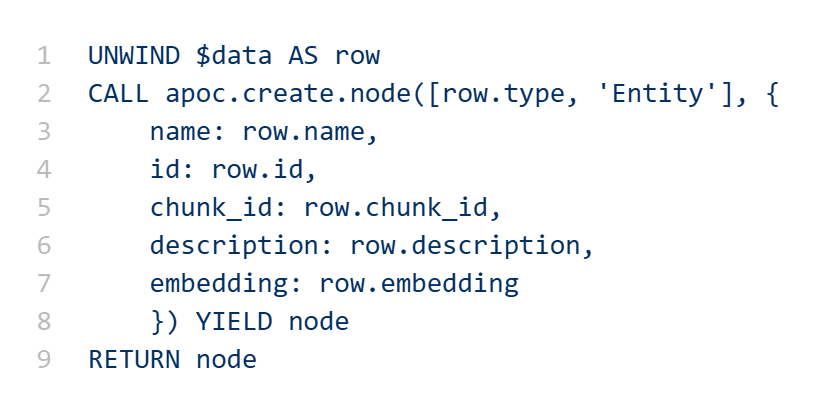
\includegraphics[width=0.8\textwidth]{images/cypher-insert-entities.png}}
	\caption{
		Kode Cypher untuk pemuatan entitas yang berupa \textit{nodes} di basis data Neo4j.
	}
	\label{fig:cypher-insert-entities}
\end{figure}

\subsection{Pengembangan Arsitektur Pengambilan Pengetahuan}
Pengambilan Pengetahuan (\textit{Knowledge Retrieval}) merupakan proses penting dalam sistem berbasis pengetahuan yang bertujuan untuk memberikan jawaban yang relevan berdasarkan pertanyaan pengguna.
\textit{Pipeline} pengambilan pengetahuan yang dikembangkan memiliki beberapa komponen utama seperti klasifikasi kueri, pencarian semantik berbasis vektor dan kata kunci, penelusuran struktur graf, serta konstruksi pengetahuan seperti pada Gambar \ref{fig:knowledge-retrieval-pipeline}.
Setiap komponen ini berkontribusi terhadap ketepatan dan relevansi hasil yang diberikan oleh sistem.

\begin{figure}[h]
	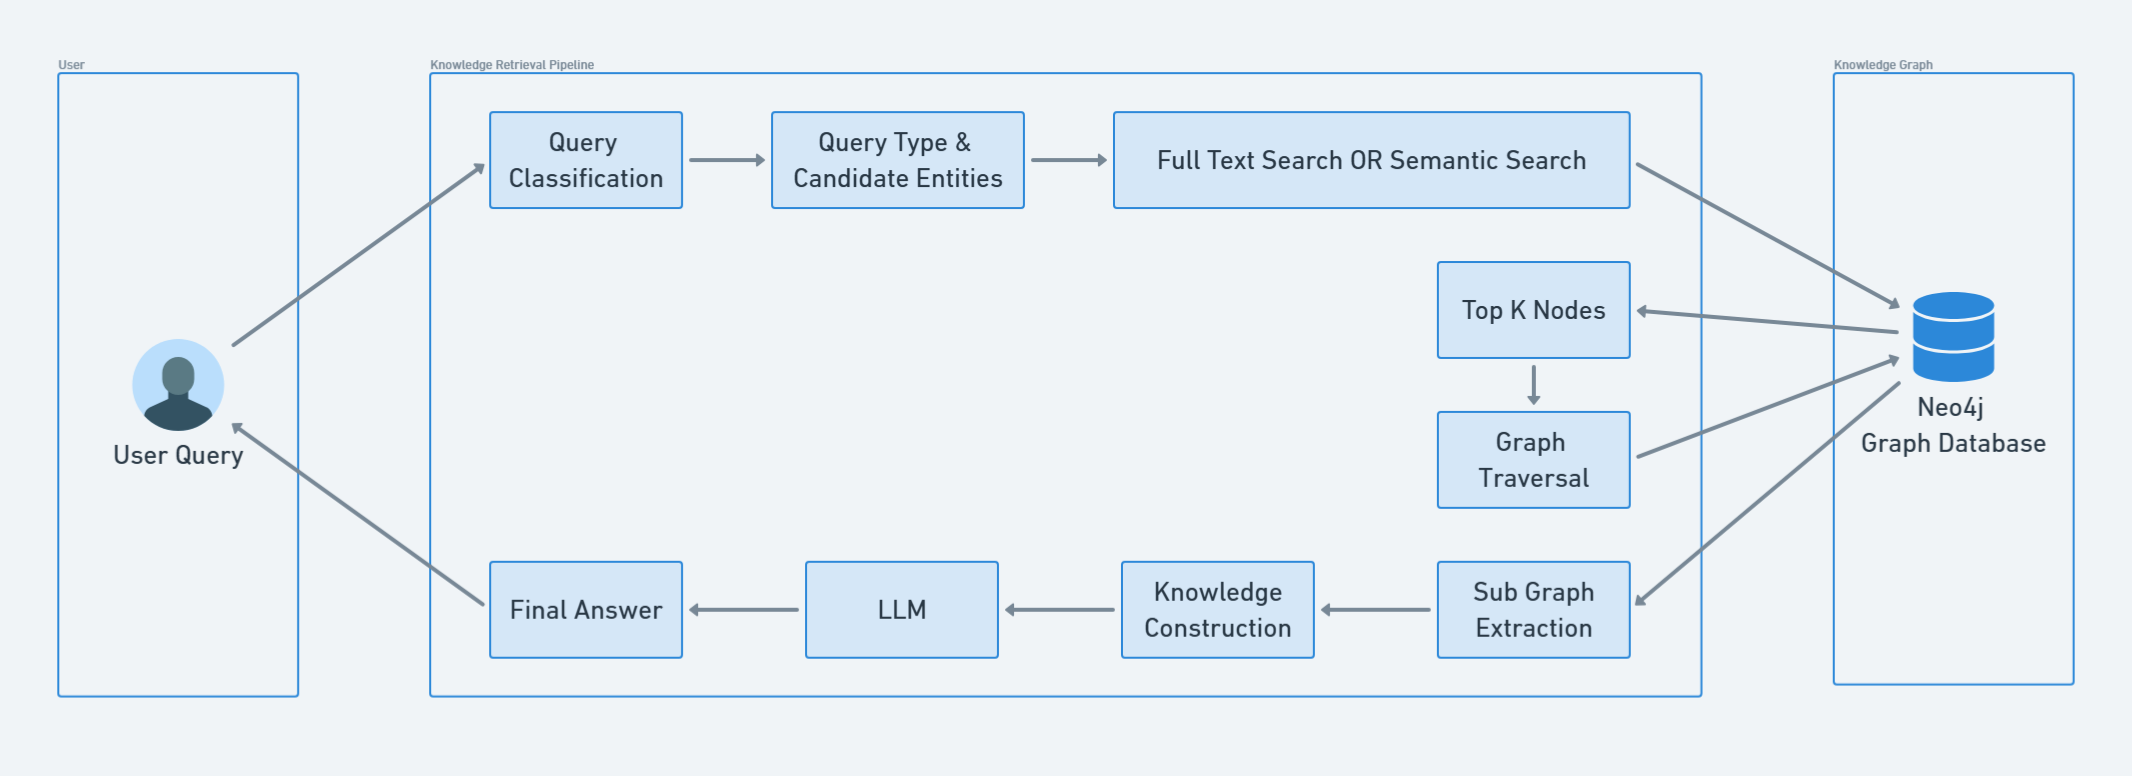
\includegraphics[width=1\textwidth]{images/knowledge-retrieval-pipeline.png}
	\caption{\textit{Pipeline Knowledge Retrieval}.}
	\label{fig:knowledge-retrieval-pipeline}
\end{figure}

\subsubsection{Klasifikasi Kueri dan Ekstraksi Entitas}
Langkah pertama dalam pengambilan pengetahuan adalah klasifikasi kueri terhadap input pengguna.
Proses ini bertujuan untuk mengidentifikasi intensi semantik dari kueri, yang nantinya akan dijadikan sebagai variabel penentu strategi pencarian dalam \textit{Knowledge Graph} yang paling sesuai.
Kueri akan diklasifikasikan menjadi dua kategori seperti pada Tabel \ref{tab:query-classification}.

\begin{table}[H]
	\centering
	\caption{Klasifikasi kueri menjadi dua kategori, yaitu \texttt{entity\_query} dan \texttt{path\_query}}
	\label{tab:query-classification}
	\begin{tabular}{|l|p{8cm}|}
		\hline
		\textbf{Kategori}      & \textbf{Keterangan}                                               \\
		\hline
		\texttt{entity\_query} &
		Jenis kueri yang berfokus pada satu entitas utama dan bertujuan untuk mendeskripsikan, mengambil atribut, atau memahami konsep dari entitas tersebut.
		Kueri ini biasanya mengandung permintaan informasi faktual atau deskriptif.                \\
		\hline
		\texttt{path\_query}   &
		Jenis kueri yang melibatkan dua atau lebih entitas, dan bertujuan untuk menelusuri hubungan atau alur keterkaitan antar entitas dalam graf.
		Kueri ini dapat digunakan untuk menemukan relasi eksplisit maupun implisit antara entitas. \\
		\hline
	\end{tabular}
\end{table}

Klasifikasi kueri ini sangat berkaitan dengan strategi pencarian yang akan dilakukan pada basis data graf.
Sebuah kueri diklasifikasikan sebagai \texttt{entity\_query} jika intensi utamanya adalah untuk mendeskripsikan atau melihat lebih detail pada satu atau beberapa konsep sentral.
Pertanyaan dari pengguna seperti \textit{"Apa itu kesehatan mental?"} atau \textit{"Di manakah pusat layanan kesehatan mental di UGM?"} termasuk dalam kategori ini karena memiliki intensi untuk tahu lebih dalam pada suatu konsep yaitu
Untuk menjawab pertanyaan tersebut, sistem hanya perlu menemukan \textit{node} \textit{"Kesehatan Mental"} dan \textit{"Pusat Layanan Kesehatan Mental UGM"} di dalam graf dan mengambil informasi yang melekat langsung padanya (deskripsi) beserta tetangga-tetangga terdekat yang berfungsi sebagai atribut.
Penelusuran ini bersifat melebar dari satu atau beberapa titik pusat.

Sebuah kueri diklasifikasikan sebagai \texttt{path\_query} apabila intensi utamanya adalah memahami relasi, interaksi, atau alur proses antara dua atau lebih konsep yang berbeda.
Pertanyaan dari pengguna seperti \textit{"Bagaimana terapi kognitif Perilaku membantu mengatasi gangguan kecemasan?"} dan \textit{"Apakah stres dapat mengakibatkan penyakit jantung?"}.
Untuk menjawab pertanyaan tersebut, sistem tidak bisa hanya melihat masing-masing \textit{nodes} dan tetangganya.
Sistem harus bisa menemukan hubungan antara beberapa \textit{nodes} lalu menelusuri jalur (\textit{path}) yang menghubungkannya.

Klasifikasi kueri memiliki peran krusial untuk menentukan bagaimana sistem akan melakukan pencarian dalam basis data graf.
Tidak seperti basis data relasional atau basis data lain yang memiliki skema terdefinisi, basis data graf dapat memiliki objek (\textit{node}) yang saling terhubung satu sama lain tanpa terikat pada skema tertentu.
Pencarian yang buruk tidak akan menghasilkan informasi yang tepat sasaran terhadap kueri pengguna.
Untuk itu strategi pencarian menjadi hal yang signifikan terhadap kualitas pengambilan pengetahuan.

Selain klasifikasi kueri, sistem akan mengekstraksi kandidat entitas yang terkandung dalam kueri.
Proses ini bertujuan untuk mengidentifikasi elemen-elemen penting dalam kueri yang berpotensi merujuk pada \textit{node} dalam basis data graf.
Ekstraksi entitas ini penting dilakukan untuk memberikan petunjuk saat melakukan pencarian dalam basis data graf.
Kandidat entitas yang berasal dari kueri pengguna akan dijadikan sebagai kata kunci dalam melakukan pencarian di samping pencarian berbasis vektor.

Proses klasifikasi kueri dan ekstraksi entitas dilakukan secara simultan menggunakan pendekatan berbasis LLM, yang mampu memahami konteks linguistik untuk mengidentifikasi istilah seperti nama penyakit, gejala, proses, atau entitas lainnya.
\textit{Prompt} disusun dengan memberikan instruksi, definisi, dan format keluaran yang diharapkan.
Selain itu, \textit{few-shot prompt} digunakan untuk memberikan contoh input dan keluaran yang diharapkan pada LLM untuk mendapatkan respons yang diinginkan seperti pada Gambar \ref{fig:prompt-query-classification-entity-extraction}.

\begin{figure}[H]
	\fbox{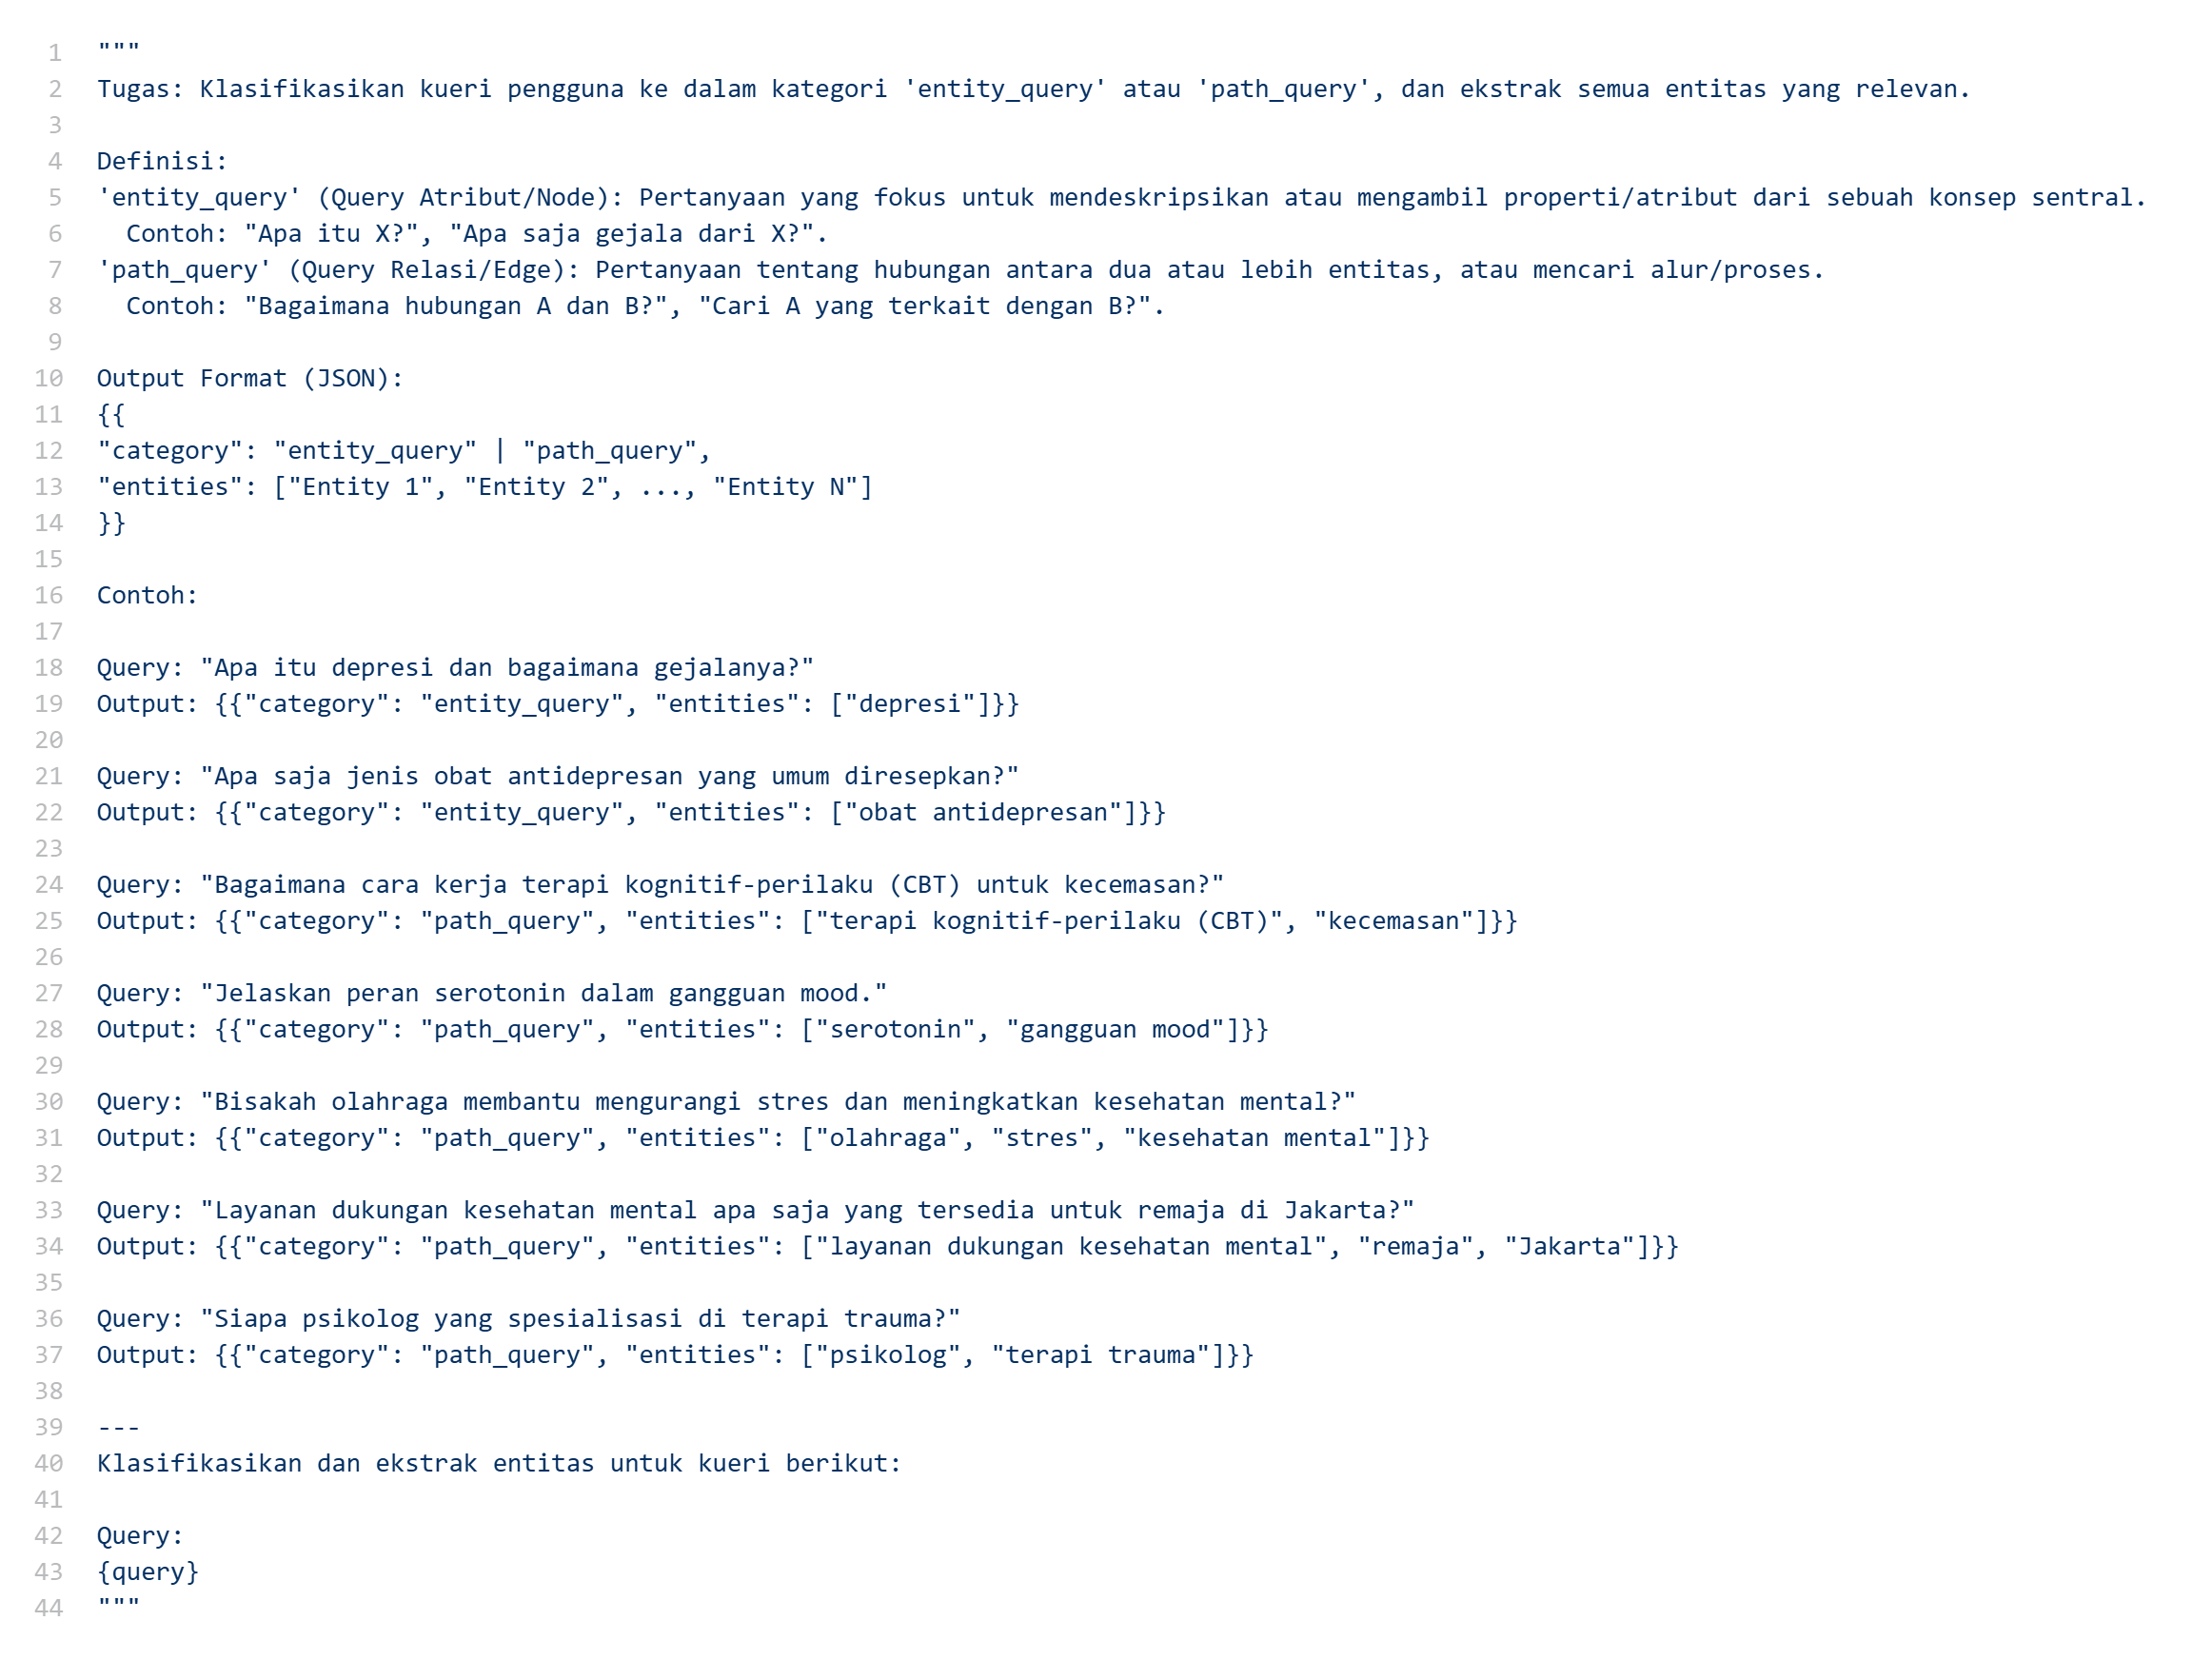
\includegraphics[width=1\textwidth]{images/prompt-query-classification-entity-extraction.png}}
	\caption{\textit{Prompt} yang digunakan untuk memberikan instruksi LLM dalam tugas klasifikasi kueri dan ekstraksi entitas}
	\label{fig:prompt-query-classification-entity-extraction}
\end{figure}

\subsubsection{\textit{Hybrid Search}}
Setelah diekstrak dari kueri pengguna pada proses sebelumnya, kandidat entitas menjadi basis untuk melakukan pencarian entitas dalam graf.
Proses pencarian ini bertujuan untuk mencari \textit{nodes} pada basis data graf yang berkaitan dengan kueri pengguna.
Pencarian didasarkan pada dua variabel utama, yaitu kandidat entitas yang telah diekstrak pada proses sebelumnya dan kueri pengguna itu sendiri.
Tahap pencarian dalam arsitektur ini menggunakan pendekatan \textit{hybrid search} yang merupakan kombinasi dua strategi pencarian, yaitu \textit{full-text search} dan \textit{semantic search} berbasis vektor.
Kedua metode ini dijalankan secara berurutan dengan strategi \textit{fallback} untuk meningkatkan efektivitas pencarian entitas dalam basis data graf.

Proses dimulai dengan melakukan pencarian entitas menggunakan \textit{full-text search} di Neo4j.
Kata kunci yang digunakan berasal dari hasil ekstraksi entitas kandidat pada tahap sebelumnya.
\textit{Full-text search} memanfaatkan indeks teks untuk mencocokkan nama \textit{node} secara eksplisit dalam basis data graf.
Pendekatan ini efektif untuk kueri yang mengandung istilah eksplisit yang cocok dengan nama entitas.

Apabila pencarian berbasis teks tidak menghasilkan entitas yang relevan, misalnya karena variasi bahasa, sinonim, atau struktur kalimat yang tidak eksplisit, maka sistem akan secara otomatis melakukan \textit{fallback} ke pencarian semantik.
Pada tahap ini, sistem mengubah kueri pengguna menjadi vektor \textit{embedding}, kemudian mencari entitas dengan representasi vektor yang paling mirip menggunakan algoritma \textit{Approximate Nearest Neighbor} (ANN) yang didukung secara \textit{native} di Neo4j, yaitu HNSW (\textit{Hierarchical Navigable Small World}).

Dari kedua metode tersebut, sistem akan memperoleh sejumlah entitas paling relevan, yaitu Top-K entitas, yang kemudian digunakan sebagai titik awal untuk proses penelusuran graf.
Pendekatan \textit{hybrid} ini memungkinkan sistem menangani berbagai variasi bentuk pertanyaan, baik yang eksplisit, maupun implisit, serta meningkatkan cakupan pencarian dalam skenario real yang tidak dapat diprediksi.

\subsubsection{Penelusuran Graf}
Setelah diperoleh dari pencarian pada tahap sebelumnya, entitas dan jenis kueri digunakan untuk melakukan penelusuran graf (\textit{graph traversal}) untuk mengumpulkan informasi kontekstual yang lebih komprehensif dari struktur graf.
Tahap ini bertujuan menghasilkan subgraf yang relevan sebagai dasar bagi penyusunan jawaban oleh sistem.
Penelusuran graf dilakukan dengan strategi yang disesuaikan dengan jenis kueri yaitu \texttt{entity\_query} dan \texttt{path\_query}.
Algoritma n-hop neighbor expansion akan digunakan untuk menelusuri graf pada tipe kueri \texttt{entity\_query}, sedangkan algoritma top k shortest path akan digunakan pada tipe kueri \texttt{path\_query}.
Penjelasan lebih lanjut mengenai dua jenis penelusuran graf terdapat pada Tabel \ref{tab:graph-traversal-strategy}.

\begin{longtable}{|p{0.3\textwidth}|p{0.65\textwidth}|}
	\caption{Klasifikasi kueri menjadi dua kategori, yaitu \texttt{entity\_query} dan \texttt{path\_query}}
	\label{tab:graph-traversal-strategy}                                                                                                                     \\
	\hline
	\textbf{Graph Traversal}          & \textbf{Keterangan}                                                                                                  \\
	\hline \hline
	\endfirsthead

	\hline
	\textbf{Graph Traversal}          & \textbf{Keterangan}                                                                                                  \\
	\hline \hline
	\endhead

	\textbf{N-hop Neighbor Expansion} &
	Untuk kueri bertipe \texttt{entity\_query}, sistem menerapkan metode N-hop \textit{Breadth-First Search} (BFS)-style \textit{Neighbor Expansion} dari \textit{node} pusat.
	Dalam sistem ini, nilai N ditetapkan sebagai 1, sehingga hanya \textit{node} tetangga langsung (\textit{one-hop neighbors}) yang diambil.
	Pendekatan ini efektif untuk menangkap atribut langsung dan relasi langsung dari suatu entitas, seperti definisi, komponen, atau karakteristik.
	Proses ini dilakukan dengan \textit{query} Cypher untuk mengambil semua \textit{node} dan \textit{edge} yang terhubung langsung dengan entitas tersebut. \\
	\hline
	\textbf{Top-K Shortest Paths}     &
	Untuk kueri bertipe \texttt{path\_query}, sistem menggunakan pendekatan Top-K \textit{Shortest Path Traversal}, yaitu menelusuri jalur terpendek antara setiap dua entitas kandidat yang dihasilkan dari proses ekstraksi entitas.
	Jalur ini dihitung berdasarkan jumlah \textit{edge} dalam graf, dengan mempertimbangkan arah dan tipe relasi.
	Pendekatan ini digunakan untuk menemukan hubungan langsung maupun tidak langsung antar entitas, serta mengidentifikasi pola keterkaitan yang bermakna.
	Sistem dapat membatasi pencarian hingga K jalur terpendek untuk menjaga efisiensi dan relevansi hasil.                                                   \\
	\hline
\end{longtable}


\subsubsection{Transformasi Konteks}

Transformasi konteks merupakan tahap penting yang menjembatani antara hasil penelusuran graf dan proses penyusunan jawaban oleh \textit{Large Language Model} (LLM).
Tahap ini bertujuan untuk mengubah representasi subgraf hasil penelusuran yang masih bersifat struktural menjadi format teks naratif yang dapat dipahami oleh LLM secara lebih efektif.

Secara teknis, transformasi dilakukan terhadap hasil kueri Cypher yang dikembalikan dalam bentuk struktur data bersarang (\textit{nested}).
Subgraf ini berisi \textit{nodes} entitas beserta relasi antar entitas, termasuk atribut seperti tipe, label, dan deskripsi.
Untuk memungkinkan LLM memproses informasi ini dengan baik, sistem mengubahnya menjadi representasi tekstual menggunakan format blok entitas beranotasi berbasis Markdown.
Format ini mempertahankan struktur semantik penting, seperti tipe entitas, arah relasi, dan deskripsi yang menyertainya.

Alasan utama transformasi ini diperlukan adalah karena LLM bekerja optimal dengan masukan berbasis teks.
Di samping itu, apabila hasil penelusuran graf digunakan secara langsung, akan banyak \textit{overhead} informasi yang sama sekali tidak diperlukan seperti nama atribut yang justru membebani LLM karena \textit{prompt} yang lebih panjang.
Representasi berbentuk teks yang kaya konteks memungkinkan LLM untuk memahami hubungan antar entitas secara utuh, berbeda dengan daftar kalimat terpisah atau output tabel sederhana.
Dengan struktur yang jelas dan eksplisit, LLM dapat melakukan \textit{reasoning} dan menjawab pertanyaan pengguna secara lebih akurat.

Implementasi dari transformasi konteks ini dilakukan melalui fungsi Python yang secara iteratif memproses hasil Cypher \textit{query} dan mengorganisasikannya ke dalam blok-blok informasi yang terstruktur, mirip dengan format dokumentasi.
Dengan pendekatan ini, subgraf dapat diinterpretasikan oleh LLM sebagai narasi pengetahuan, bukan sekadar data mentah, sehingga meningkatkan relevansi dan presisi jawaban yang dihasilkan.

\subsubsection{Respons Final}
Tahap akhir dari arsitektur pengambilan pengetahuan adalah penyusunan jawaban akhir (\textit{final answer}) yang dikembalikan kepada pengguna.
Pada tahap ini, representasi kontekstual yang telah ditransformasikan dari subgraf sebelumnya diproses oleh LLM untuk membentuk jawaban dalam bentuk teks alami yang informatif, ringkas, dan relevan terhadap kueri pengguna.

LLM digunakan sebagai komponen generatif yang memanfaatkan informasi terstruktur yang telah diformat menjadi teks.
Dengan input yang kaya konteks, termasuk anotasi entitas, deskripsi, dan relasi antar \textit{node}-LLM dapat melakukan \textit{reasoning} semantik untuk menghasilkan jawaban yang tidak hanya berbasis fakta, tetapi juga disampaikan dalam bahasa yang mudah dipahami.

Sistem dapat mengatur gaya dan format jawaban yang dihasilkan, seperti bahasa formal atau santai sesuai kebutuhan aplikasi, panjang jawaban (ringkas vs. naratif), dan penyisipan kutipan entitas atau sumber dari graf, jika diperlukan.
Proses ini dilakukan secara deterministik (menggunakan \textit{prompt engineering} dengan temperatur rendah) untuk memastikan konsistensi dan menghindari halusinasi jawaban yang tidak berdasarkan pada data yang tersedia dalam graf.
Dengan pendekatan ini, sistem tidak hanya berfungsi sebagai pencari informasi (\textit{retriever}), tetapi juga sebagai penyaji pengetahuan yang mampu menyusun informasi menjadi jawaban utuh yang siap dikonsumsi pengguna.

\subsection{Evaluasi dan Analisis}
Tahapan evaluasi dan analisis merupakan fase krusial untuk mengukur performa sistem \textit{Retrieval-Augmented Generation} (RAG) berbasis \textit{Knowledge Graph} yang telah dibangun.
Sistem RAG ini terdiri dari dua komponen utama, yaitu sistem \textit{retrieval} yang bertugas mengambil konteks yang relevan dengan pertanyaan dan sistem \textit{generation} yang menghasilkan respons akhir.
Untuk itu, evaluasi dilakukan pada kedua komponen tersebut.

\subsubsection{Penyiapan \textit{Dataset} Evaluasi}
Salah satu tantangan dalam mengevaluasi sistem RAG adalah ketiadaan \textit{dataset} percakapan yang secara khusus sesuai dengan domain dan karakteristik dokumen yang digunakan.
Tidak seperti metode \textit{fine-tuning} yang sejak awal menggunakan data percakapan, RAG cukup memerlukan dokumennya saja.
Untuk menjawab tantangan tersebut, dilakukan pembuatan \textit{dataset} evaluasi sintesis mandiri yang seolah-olah meniru tanya jawab dengan pengguna.
Pendekatan ini dimaksudkan agar evaluasi cukup akurat mengukur kemampuan sistem dalam menjawab pertanyaan berdasarkan korpus pengetahuan yang telah diindeks.

Data percakapan untuk evaluasi dibuat berdasarkan dokumen yang dipakai untuk membangun \textit{Knowledge Graph} yang berupa potongan-potongan dokumen (\textit{document chunks}).
Setiap potongan dokumen tersebut dianggap sebagai dasar kebenaran (\textit{ground truth}) untuk menghasilkan beberapa \textit{dataset} evaluasi.
Selain potongan dokumen, \textit{Knowledge Graph} juga berperan dalam membentuk \textit{dataset} evaluasi, khususnya untuk evaluasi bagian sistem \textit{retrieval}.

Sistem akan melakukan iterasi pada setiap potongan dokumen yang telah diindeks disertai dengan \textit{nodes} dari subgraf yang berasosiasi sebagai konteks.
Konteks tersebut kemudian dimasukkan ke dalam \textit{Large Language Model} (LLM) dengan instruksi atau \textit{prompt} yang telah dirancang.
\textit{Prompt} tersebut meminta LLM untuk berperan sebagai seorang ahli pembuatan data untuk menghasilkan \textit{dataset} evaluasi yang terdiri dari beberapa \textit{field} seperti pada Tabel \ref{tab:evaluation-dataset-fields}.

\begin{table}[h]
	\centering
	\caption{\textit{Fields} pada \textit{dataset} evaluasi}
	\label{tab:evaluation-dataset-fields}
	\begin{tabular}{|p{0.3\textwidth}|p{0.6\textwidth}|}
		\hline
		\textbf{\textit{Fields}} & \textbf{Keterangan}                                                                                    \\
		\hline
		\texttt{query}           &
		\textit{Query} adalah sebuah pertanyaan yang jawabannya dapat ditemukan dari konteks yang disediakan.                             \\
		\hline
		\texttt{query\_lable}    &
		\textit{Query lable} adalah kategori kueri yang nilainya dapat berupa \textit{entity query} atau \textit{path query}.             \\
		\hline
		\texttt{golden\_nodes}   &
		\textit{Golden nodes} adalah \textit{nodes} yang berasal dari \textit{knowledge graph} yang diperlukan untuk menjawab pertanyaan. \\
		\hline
		\texttt{golden\_answer}  &
		\textit{Golden answer} merupakan jawaban akurat dari kueri dan didasarkan pada konteks yang tersedia.                             \\
		\hline
	\end{tabular}
\end{table}

Selain itu, teknik \textit{few-shot} digunakan pada \textit{prompt} untuk memberikan beberapa contoh data evaluasi yang diharapkan.
Dalam setiap potongan dokumen akan dihasilkan pertanyaan setidaknya setengah dari jumlah \textit{nodes} yang tersedia.
Jumlah tersebut dipilih guna memberikan keleluasaan LLM untuk memberikan variasi pertanyaan dan tidak terpaku bahwa setiap \textit{node} harus memiliki satu pertanyaan.

\textit{Prompt} yang sudah dirancang kemudian dieksekusi dengan model OpenAI \texttt{o4-mini}.
Pemilihan model dari OpenAI didasarkan pada model yang digunakan dalam proses evaluasi harus berbeda dengan model yang digunakan pada operasional.
Hal tersebut dilakukan guna menghindari bias dalam evaluasi apabila model yang sama digunakan dalam menjawab pertanyaan sekaligus evaluasi.
Model OpenAI \texttt{o4-mini} merupakan salah satu model kekinian yang dioptimalkan untuk tugas \textit{reasoning} yang cepat.
Kelebihan tersebut sangat sesuai dengan kebutuhan membuat \textit{dataset} evaluasi berdasarkan instruksi.

\subsubsection{Evaluasi Sistem \textit{Retrieval}}
Evaluasi sistem \textit{retrieval} bertujuan untuk mencari tahu seberapa efektif komponen \textit{retriever} dalam menghasilkan konteks yang bersesuaian.
Konteks memiliki peranan yang krusial bagi komponen generatif dalam menghasilkan jawaban akhir yang memiliki landasan informasi akurat.
Kualitas jawaban akhir yang dihasilkan secara signifikan dipengaruhi oleh relevansi dan kelengkapan konteks yang disediakan.
Apabila \textit{retriever} gagal menemukan konteks yang tepat, maka jawaban akhir akan berisiko tidak akurat bahkan cenderung menghasilkan "halusinasi", yaitu informasi yang tidak didasarkan pada data faktual.
Halusinasi ini menjadi masalah besar terlebih apabila sistem ini akan diterapkan sebagai \textit{chatbot} layanan kesehatan mental yang penggunanya sering berhubungan langsung dengan pasien yang memiliki risiko mental.
Kesalahan informasi dapat mengakibatkan dampak yang fatal baik bagi penderita kesehatan mental ataupun bagi pengguna pada umumnya.

Dalam kasus RAG berbasis \textit{Knowledge Graph}, konteks berarti subgraf yang dihasilkan oleh \textit{retriever}.
Setiap kali sistem menjawab pertanyaan, subgraf yang berkaitan dengan pertanyaan akan diambil dari basis data.
Subgraf tersebut terdiri dari dua komponen yaitu \textit{node} yang berisi informasi entitas dan \textit{edge} yang berupa relasi antar entitas.
Dalam proses evaluasi ini, hanya komponen nama  \textit{node} yang digunakan dengan asumsi bahwa \textit{nodes} yang dihasilkan sudah mewakili konteks informasi.
Hal tersebut dilakukan untuk menyederhanakan evaluasi dengan membandingkan \textit{nodes} yang dihasilkan dengan \textit{golden nodes} pada \textit{dataset} evaluasi sebagai \textit{ground truth}.
Untuk setiap pertanyaan, sistem \textit{retrieval} akan diminta untuk mengambil n subgraf yang relevan dengan pertanyaan.
Bentuk dari subgraf terbagi menjadi dua kategori berdasarkan jenis pertanyaannya, yaitu \textit{neighbor expansion} dan n \textit{shortest path}.
Masing-masing jenis subgraf tersebut memiliki struktur yang berbeda, tetapi tidak menjadi masalah karena hanya diambil nama \textit{nodes} yang terkandung di dalamnya.
\textit{Nodes} tersebut kemudian dibandingkan dengan \textit{golden nodes} untuk menghasilkan sejumlah metrik kuantitatif seperti pada Tabel \ref{tab:retrieval-evaluation-metrics} yang digunakan untuk mengukur efektivitas sistem \textit{retrieval}.

\begin{table}[H]
	\centering
	\caption{Metrik evaluasi sistem \textit{Retrieval} }
	\label{tab:retrieval-evaluation-metrics}
	\begin{tabular}{|p{0.2\textwidth}|p{0.7\textwidth}|}
		\hline
		\textbf{Metrik}                              & \textbf{Keterangan}                                                                                                                                                                                                                                    \\
		\hline
		\textbf{\textit{Precision}}                  &
		Presisi mengukur proporsi \textit{nodes} yang relevan di antara \textit{nodes} yang dihasilkan oleh \textit{retriever}. Metrik ini menjawab pertanyaan \textit{"Seberapa banyak dari hasil yang diberikan oleh sistem yang benar-benar berkaitan?"}.                                                  \\
		\hline
		\textbf{\textit{Recall}}                     &
		\textit{Recall} mengukur proporsi \textit{nodes} relevan yang berhasil ditemukan dari semua \textit{nodes} relevan yang tersedia. Metrik ini menjawab pertanyaan \textit{"Seberapa lengkap cakupan hasil yang diberikan oleh sistem?"}.                                                               \\
		\hline
		\textbf{\textit{Hit Ratio}}                  &
		\textit{Hit Ratio} mengukur apakah setidaknya satu \textit{node} yang relevan berada di antara $k$ hasil teratas yang dikembalikan. Ini adalah metrik biner yang hanya peduli apakah jawaban yang benar ada di dalam daftar hasil, tidak peduli di peringkat berapa.                                  \\
		\hline
		\textbf{\textit{Mean Reciprocal Rank} (MRR)} &
		\textit{Mean Reciprocal Rank} (MRR) mengukur seberapa cepat sistem memprioritaskan \textit{nodes} yang relevan. Metrik ini berfokus pada dokumen peringkat dari \textit{node} relevan pertama yang ditemukan. Skor tinggi menunjukkan sistem memprioritaskan \textit{node} relevan di peringkat atas. \\
		\hline
	\end{tabular}
\end{table}

\subsubsection{Evaluasi Respons Akhir}
Evaluasi respons akhir berfokus pada penilaian terhadap kualitas jawaban akhir yang dihasilkan sistem, khususnya pada bagian generatif setelah menerima konteks dari komponen \textit{retrieval}.
Evaluasi ini mempertimbangkan beberapa parameter penting, antara lain faktualitas, relevansi, dan kebenaran jawaban, guna memastikan bahwa respons akhir yang diberikan kepada pengguna memiliki nilai informatif yang tinggi dan sesuai dengan pertanyaan yang diajukan.

Keberhasilan sistem RAG tidak hanya ditentukan oleh kemampuan dalam mengambil konteks yang relevan, tetapi juga oleh kemampuan LLM dalam menghasilkan jawaban yang benar dan relevan berdasarkan konteks tersebut.
Dalam beberapa kasus, bahkan jika konteks yang diambil sudah tepat, model generatif dapat tetap menghasilkan jawaban yang tidak faktual, tidak tepat sasaran, atau terlalu umum.
Oleh karena itu, evaluasi terhadap respons akhir menjadi sangat penting untuk menilai efektivitas akhir sistem RAG secara holistik, mendeteksi adanya halusinasi, dan menjamin bahwa jawaban benar-benar menjawab pertanyaan pengguna secara akurat.

\vspace{1cm}
Evaluasi dilakukan dengan menggunakan \textit{framework} RAGAS (\textit{Retrieval-Augmented Generation Assessment}), yaitu sebuah kerangka kerja modern dan terstandardisasi yang dirancang khusus untuk mengevaluasi \textit{pipeline} RAG secara menyeluruh.
RAGAS akan menghitung sejumlah metrik evaluasi terhadap jawaban yang dihasilkan dengan membandingkannya terhadap \textit{golden answer} dan konteks. Pendekatan ini memungkinkan evaluasi yang kuantitatif, objektif, dan replikatif.
Metrik yang digunakan untuk menilai kualitas jawaban akhir terdapat pada Tabel \ref{tab:generation-evaluation-metrics}.

\begin{table}[h]
	\centering
	\caption{Metrik evaluasi sistem \textit{Generation} }
	\label{tab:generation-evaluation-metrics}
	\begin{tabular}{|p{0.2\textwidth}|p{0.7\textwidth}|}
		\hline
		\textbf{Metrik}                               & \textbf{Keterangan}                                                                               \\
		\hline
		\textbf{\textit{Faithfulness}}                &
		Mengukur sejauh mana jawaban yang dihasilkan tetap berpegang pada informasi dalam konteks.
		Skor tinggi menunjukkan bahwa jawaban tidak mengandung halusinasi.                                                                                \\
		\hline
		\textbf{\textit{Answe \newline Relevancy}}    &
		Menilai apakah jawaban benar-benar menjawab pertanyaan yang diajukan.
		Jawaban faktual tetapi tidak menjawab pertanyaan secara langsung akan memiliki skor rendah.                                                       \\
		\hline
		\textbf{\textit{Answer \newline Correctness}} &
		Membandingkan jawaban yang dihasilkan dengan \textit{golden answer} untuk mengukur kesesuaian dan kebenaran faktual.
		Ini merupakan indikator langsung dari akurasi jawaban.                                                                                            \\
		\hline
		\textbf{\textit{Answer\newline Similarity}}   &
		Mengukur kemiripan semantik antara jawaban yang dihasilkan dan \textit{golden answer} menggunakan \textit{cosine similarity} atas representasi vektor dari kedua jawaban.
		Skor tinggi menunjukkan bahwa secara makna, jawaban yang dihasilkan sangat mirip dengan \textit{golden answer}, meskipun berbeda secara tekstual. \\
		\hline
	\end{tabular}
\end{table}
\cleardoublepage \phantomsection
\chapter{Hasil dan Pembahasan}

Bab ini menyajikan hasil dan analisis mendalam terhadap sistem RAG berbasis \textit{Knowledge Graph} yang telah dirancang dan diimplementasikan.
Penyajian dimulai dari tahap ekstraksi dan penyerapan pengetahuan dari korpus dokumen.
Selanjutnya dipaparkan hasil evaluasi kuantitatif dari rancangan arsitektur RAG, baik pada komponen \textit{retriever}, maupun jawaban final yang dihasilkan oleh sistem secara keseluruhan.
Setiap hasil akan diikuti dengan pembahasan untuk menginterpretasikan data, menganalisis kekuatan dan kelemahan sistem, serta menyajikan studi kasus untuk memberikan gambaran yang lebih jelas.

\section{Hasil \textit{Knowledge Extraction}}
Proses \textit{knowledge extraction} dimulai dengan ekstraksi teks dari dokumen.
Dokumen yang dalam format HTML atau DOCX kemudian diambil teks yang terkandung di dalamnya sekaligus dilakukan \textit{structural chunking} untuk membaginya ke dalam beberapa potongan berdasarkan tingkatan hierarki tertentu.
Proses \textit{chunking} hanya dilakukan pada dokumen buku "Petunjuk Teknis Pencegahan dan Pengendalian Gangguan Mental Emosional" karena berukuran cukup besar, yaitu sekitar 15.000 kata, dibandingkan dengan dokumen lainnya yang kurang dari 6.000 kata.
Hal tersebut dilakukan mengingat LLM kesulitan untuk secara detail memahami isi dari dokumen tersebut.
Dari proses \textit{chunking} tersebut menghasilkan total 17 potongan dokumen yang disimpan dalam format TXT.

Sejumlah 17 potongan dokumen tersebut kemudian dimasukkan ke dalam LLM untuk diekstrak entitas dan relasi yang terkandung secara berurutan.
Dari proses ekstraksi tersebut menghasilkan 1.119 entitas dan 1.078 relasi secara keseluruhan.
Tabel \ref{tab:knowledge-graph-stats} menunjukkan statistik \textit{Knowledge Graph} yang dihasilkan dari dokumen secara keseluruhan

\begin{table}[h]
	\centering
	\caption{Statistik \textit{Knowledge Graph} yang dihasilkan dari dokumen}
	\label{tab:knowledge-graph-stats}
	{\setlength{\tabcolsep}{0.5em}
		\begin{tabular}{|l|r|}
			\hline
			\textbf{Komponen}         & \textbf{Jumlah} \\
			\hline \hline
			\textbf{Dokumen}          &
			5                                           \\
			\hline
			\textbf{Potongan Dokumen} &
			17                                          \\
			\hline
			\textbf{Entitas}          &
			1119                                        \\
			\hline
			\textbf{Relasi}           &
			1073                                        \\
			\hline
			\textbf{Jenis Entitas}    &
			18                                          \\
			\hline
			\textbf{Jenis Relasi}     &
			18                                          \\
			\hline
		\end{tabular}}
\end{table}


Suatu fakta yang berhasil diekstrak dari dokumen akan disimpan dalam bentuk triplet (subjek, predikat, dan objek), yang kemudian diimplementasikan sebagai \textit{node} dan \textit{edge} dalam struktur graf pengetahuan.
Sebagai contoh, berikut adalah sebuah potongan dokumen yang dianalisis:

\begin{quote}
	\itshape
	Faktor psikologis yaitu kegagalan, kekecewaan, trauma yang mengakibatkan stres dan faktor biologis yaitu genetik, gizi dan infeksi perinatal serta kondisi lingkungan yang buruk juga merupakan faktor yang berkontribusi terhadap terjadinya gangguan jiwa.

	\textbf{Faktor Psikologis} \\
	Faktor psikologis yang menjadi faktor risiko GME, antara lain (Kerig, Ludlow, \& Wenar, 2012; PPSDM Kemenkes RI, 2016):
	\begin{enumerate}
		\item Regulasi emosi rendah
		\item Kemampuan regulasi diri rendah yang termanifestasikan dalam kontrol perilaku yang buruk
		\item Konsep diri negatif
		\item Efikasi diri rendah
		\item Resiliensi diri rendah
	\end{enumerate}

	\textbf{Cara menangani Resiliensi Diri Rendah:}
	\begin{enumerate}[label=\alph*)]
		\item Melatih keterampilan manajemen stres
		\item Melatih fleksibilitas dalam berpikir dan keterampilan pengambilan keputusan
		\item Melatih keterampilan manajemen konflik
	\end{enumerate}
	\normalfont
\end{quote}

Berdasarkan potongan dokumen tersebut, sistem ekstraksi menghasilkan beberapa triplet pengetahuan sebagai berikut:

\begin{lstlisting}[frame=single, numbers=none, basicstyle=\ttfamily\footnotesize]
(:Gangguan_Mental {name: "Gangguan Jiwa"})<-[:Berkontribusi_Pada]-(:Faktor_Risiko {name: "Faktor Psikologis"})

(:Gangguan_Mental {name: "Gangguan Jiwa"})<-[:Berkontribusi_Pada]-(:Faktor_Risiko {name: "Faktor Biologis"})

(:Gejala {name: "Resiliensi Diri Rendah"})-[:Adalah_Jenis_Dari]->(:Faktor_Risiko {name: "Faktor Psikologis"})

(:Aktivitas_Kesejahteraan {name: "Manajemen Konflik"})-[:Menangani]->(:Gejala {name: "Resiliensi Diri Rendah"})

(:Aktivitas_Kesejahteraan {name: "Keterampilan Pengambilan Keputusan"})-[:Menangani]->(:Gejala {name: "Resiliensi Diri Rendah"})
\end{lstlisting}

\section{Hasil Pengembangan Arsitektur RAG Berbasis \textit{Knowledge Graph}}

Sistem yang dikembangkan berupa AI \textit{service} berbasis arsitektur RAG-KG.
Layanan AI tersebut disediakan dalam bentuk REST API sehingga memudahkan dalam integrasi dengan platform lain.
Antarmuka aplikasi REST juga memudahkan dalam pengujian dan menyimulasikan sistem ketika diimplementasikan pada skenario penggunaan sebenarnya.
Arsitektur dirancang untuk mendukung proses penjawaban pertanyaan yang memprioritaskan jawaban berbasis konteks.
Basis konteks tersebut diperoleh dari pengambilan informasi pada \textit{Knowledge Graph} dengan memanfaatkan entitas dan relasi yang terkandung di dalamnya.
AI \textit{service} dapat diakses melalui HTTP \textit{request} dengan spesifikasi seperti pada Tabel \ref{tab:ai-service-answer}.

\begin{longtable}{|p{0.3\textwidth}|p{0.65\textwidth}|}
	\caption{Spesifikasi \textit{endpoint} untuk menghasilkan jawaban}
	\label{tab:ai-service-answer}                                                               \\
	\hline
	\textbf{Komponen}             & \textbf{Nilai}                                              \\
	\hline \hline
	\endfirsthead

	\hline
	\textbf{Komponen}             & \textbf{Nilai}                                              \\
	\hline \hline
	\endhead


	\textbf{URL}                  &
	http://localhost:8080/api/v1/retrieval/get-answer                                           \\
	\hline
	\textbf{HTTP \textit{Method}} &
	POST                                                                                        \\
	\hline
	\textbf{\textit{Body} (JSON)} & \begin{lstlisting}[basicstyle=\ttfamily\small, numbers=none]
{
  "query": "",
  "graph_traversal": "",
  "search_method": "",
  "max_hop": 0,
  "limit": 0,
  "top_k": 0
}
    \end{lstlisting} \\
	\hline
	\textbf{Respons (JSON)}       & \begin{lstlisting}[basicstyle=\ttfamily\small, numbers=none]
{
  "message": "",
  "data": {
    "latency" : 0.0,
    "method": "",
    "query_class": {
      "category": "",
      "entities": []
    },
    "answer" : "",
    "knowledge": "",
    "graph" : {}
  }
}
    \end{lstlisting} \\
	\hline
\end{longtable}

Untuk memperoleh respons dari sistem dilakukan pemanggilan API dengan spesifikasi seperti pada Tabel \ref{tab:ai-service-answer}.
Berikut merupakan potongan contoh respons sistem untuk pertanyaan \textit{"Apa itu Gangguan Mental Emosional?"} pada Tabel \ref{tab:ai-service-response-example}.

\begin{longtable}{|p{0.2\textwidth}|p{0.7\textwidth}|}
	\caption{Contoh respons sistem dalam menghasilkan jawaban}
	\label{tab:ai-service-response-example}                                                    \\
	\hline
	\textbf{Komponen}            & \textbf{Isi}                                                \\
	\hline \hline
	\endfirsthead

	\hline
	\textbf{Komponen}            & \textbf{Isi}                                                \\
	\hline \hline
	\endhead


	Kueri                        &
	Apa itu Gangguan Mental Emosional?                                                         \\
	\hline
	\textit{Request Body}        & \begin{lstlisting}[basicstyle=\ttfamily\small, numbers=none]
{
  "query": "Apa itu Gangguan Mental Emosional?",
  "graph_traversal": "auto",
  "search_method": "auto",
  "max_hop": 10,
  "limit": 50,
  "top_k": 3
}
    \end{lstlisting} \\
	\hline
	Konteks \newline Pengetahuan &
	Berikut adalah informasi yang ditemukan dari knowledge graph:

	\textbf{Entitas: Gangguan Mental Emosional} (Tipe: Gangguan\_Mental)
	\begin{itemize}
		\item Deskripsi: Bukan diagnosis gangguan jiwa.
		      Dapat memengaruhi aktifitas sehari-hari yang berdampak pada menurunnya produktifitas dan kualitas hidup.
		      Kondisi atau gangguan yang menjadi subjek utama dari 'Petunjuk Teknis Pencegahan dan Pengendalian Gangguan Mental Emosional'.
		      ....
		\item Skor Relevansi Awal: 5.07
		\item Hubungan Terkait:
		      \begin{itemize}
			      \item[$\rightarrow$] \textsl{merupakan} $\rightarrow$ Masalah Kesehatan Jiwa
			      \item[$\rightarrow$] \textsl{mengindikasikan} $\rightarrow$ Perubahan Psikologis
			      \item[$\leftarrow$] \textsl{mencegah} $\leftarrow$ Upaya Promosi Kesehatan
			      \item [...]
		      \end{itemize}
	\end{itemize}
	\textbf{Entitas: Deteksi Gangguan Mental Emosional} (Tipe: Layanan\_Kesehatan)
	\begin{itemize}
		\item Deskripsi: Proses identifikasi gangguan mental emosional yang diharapkan mampu dilakukan oleh fasilitas pelayanan kesehatan primer.
		\item Skor Relevansi Awal: 4.52
		\item Hubungan Terkait:
		      \begin{itemize}
			      \item[$\leftarrow$] \textsl{mampu melakukan} $\leftarrow$ Fasilitas pelayanan kesehatan primer
			      \item[$\rightarrow$] \textsl{dapat segera diintervensi} $\rightarrow$ Intervensi
			      \item[...]
		      \end{itemize}
	\end{itemize}
	\textbf{Penderita Gangguan Mental Emosional} (Tipe: Individu)
	\begin{itemize}
		\item Deskripsi: Proses identifikasi gangguan mental emosional yang diharapkan mampu dilakukan oleh fasilitas pelayanan kesehatan primer.
		      ... (Informasi selengkapnya dapat dilihat pada Lampiran)
	\end{itemize}
	\\
	\hline

	Jawaban                      &
	Gangguan Mental Emosional (GME) adalah suatu kondisi yang mengindikasikan seseorang mengalami perubahan psikologis. Perubahan ini bisa merupakan kondisi normal, namun dapat juga merupakan kondisi patologis.

	Penting untuk diketahui bahwa Gangguan Mental Emosional \textbf{bukanlah diagnosis gangguan jiwa}. Meskipun demikian, kondisi ini merupakan masalah kesehatan jiwa yang banyak dijumpai di Indonesia, diperkirakan diderita oleh 19 juta orang.

	GME dapat memengaruhi aktivitas sehari-hari seseorang, yang pada akhirnya berdampak pada menurunnya produktivitas dan kualitas hidup. Istilah ini juga digunakan dalam ``Petunjuk Teknis Pencegahan dan Pengendalian Gangguan Mental Emosional'' sebagai subjek utama panduan tersebut.
	\\
	\hline
\end{longtable}

Pada potongan contoh respons sistem untuk pertanyaan \textit{"Apa itu Gangguan Mental Emosional"} pada tabel \ref{tab:ai-service-response-example}, sistem akan mengambil konteks pengetahuan yang diperoleh dari \textit{Knowledge Graph}.
Terlihat dalam konteks pengetahuan yang diambil sistem berhasil mengambil beberapa entitas utama (Gangguan Mental Emosional, Deteksi Gangguan Mental Emosional, dan Penderita Gangguan Mental Emosional) beserta entitas tetangganya.
Konteks pengetahuan yang diperoleh tidak hanya menyediakan definisi, tetapi juga relasi antar entitas, seperti "merupakan", "mengindikasikan", dan "mencegah".
Hal tersebut sangat penting untuk menyediakan konteks bagi LLM sehingga mampu menghasilkan jawaban yang holistik.
Jawaban yang dihasilkan tidak hanya menjawab pertanyaan \textit{"Apa itu Gangguan Mental Emosional?"} secara langsung, tetapi juga memberikan informasi tambahan yang relevan dan penting.
Jawaban akhir secara langsung merefleksikan dan menyintesis informasi yang ada di dalam konteks pengetahuan, membuktikan bahwa sistem tidak berhalusinasi, setidaknya pada contoh ini.

\section{Hasil Pengembangan \textit{Dataset} Evaluasi Sitetis}
\textit{Dataset} evaluasi diperoleh secara sintesis melalui proses \textit{prompting} pada model OpenAI o4-mini.
Data yang dihasilkan berupa pasangan \textit{query} atau pertanyaan dan \textit{golden answer} atau jawaban yang dianggap sebagai acuan jawaban yang diharapkan.
Selain itu dibubuhkan juga \textit{golden nodes} yang merujuk pada \textit{nodes} yang relevan untuk menjawab pertanyaan dan \texttt{query\_lable} untuk menandai jenis pertanyaan.
Dari proses \textit{prompting} diperoleh hasil berupa 433 data evaluasi yang terdiri dari 266 \texttt{entity\_query} dan 167 \texttt{path\_query} seperti pada Tabel \ref{tab:evaluation-dataset-result}.
Setiap pertanyaan tersebut dijamin memiliki referensi ke setidaknya satu \textit{node} dalam \textit{Knowledge Graph}.
Contoh \textit{dataset} sintesis yang dihasilkan dapat dilihat pada Gambar \ref{fig:evaluation-dataset-example}.

\begin{table}[H]
	\centering
	\caption{Hasil sintesis \textit{dataset} evaluasi menggunakan model OpenAI o4-mini}
	\label{tab:evaluation-dataset-result}
	\begin{tabular}{|l|r|}
		\hline
		\textbf{Kategori Kueri} & \textbf{Jumlah} \\
		\hline \hline
		\texttt{entity\_query}  &
		266                                       \\
		\hline
		\texttt{path\_query}    &
		167                                       \\
		\hline
		\textbf{Total}          &
		433                                       \\
		\hline
	\end{tabular}
\end{table}


\begin{figure}[H]
	\centering
	\fbox{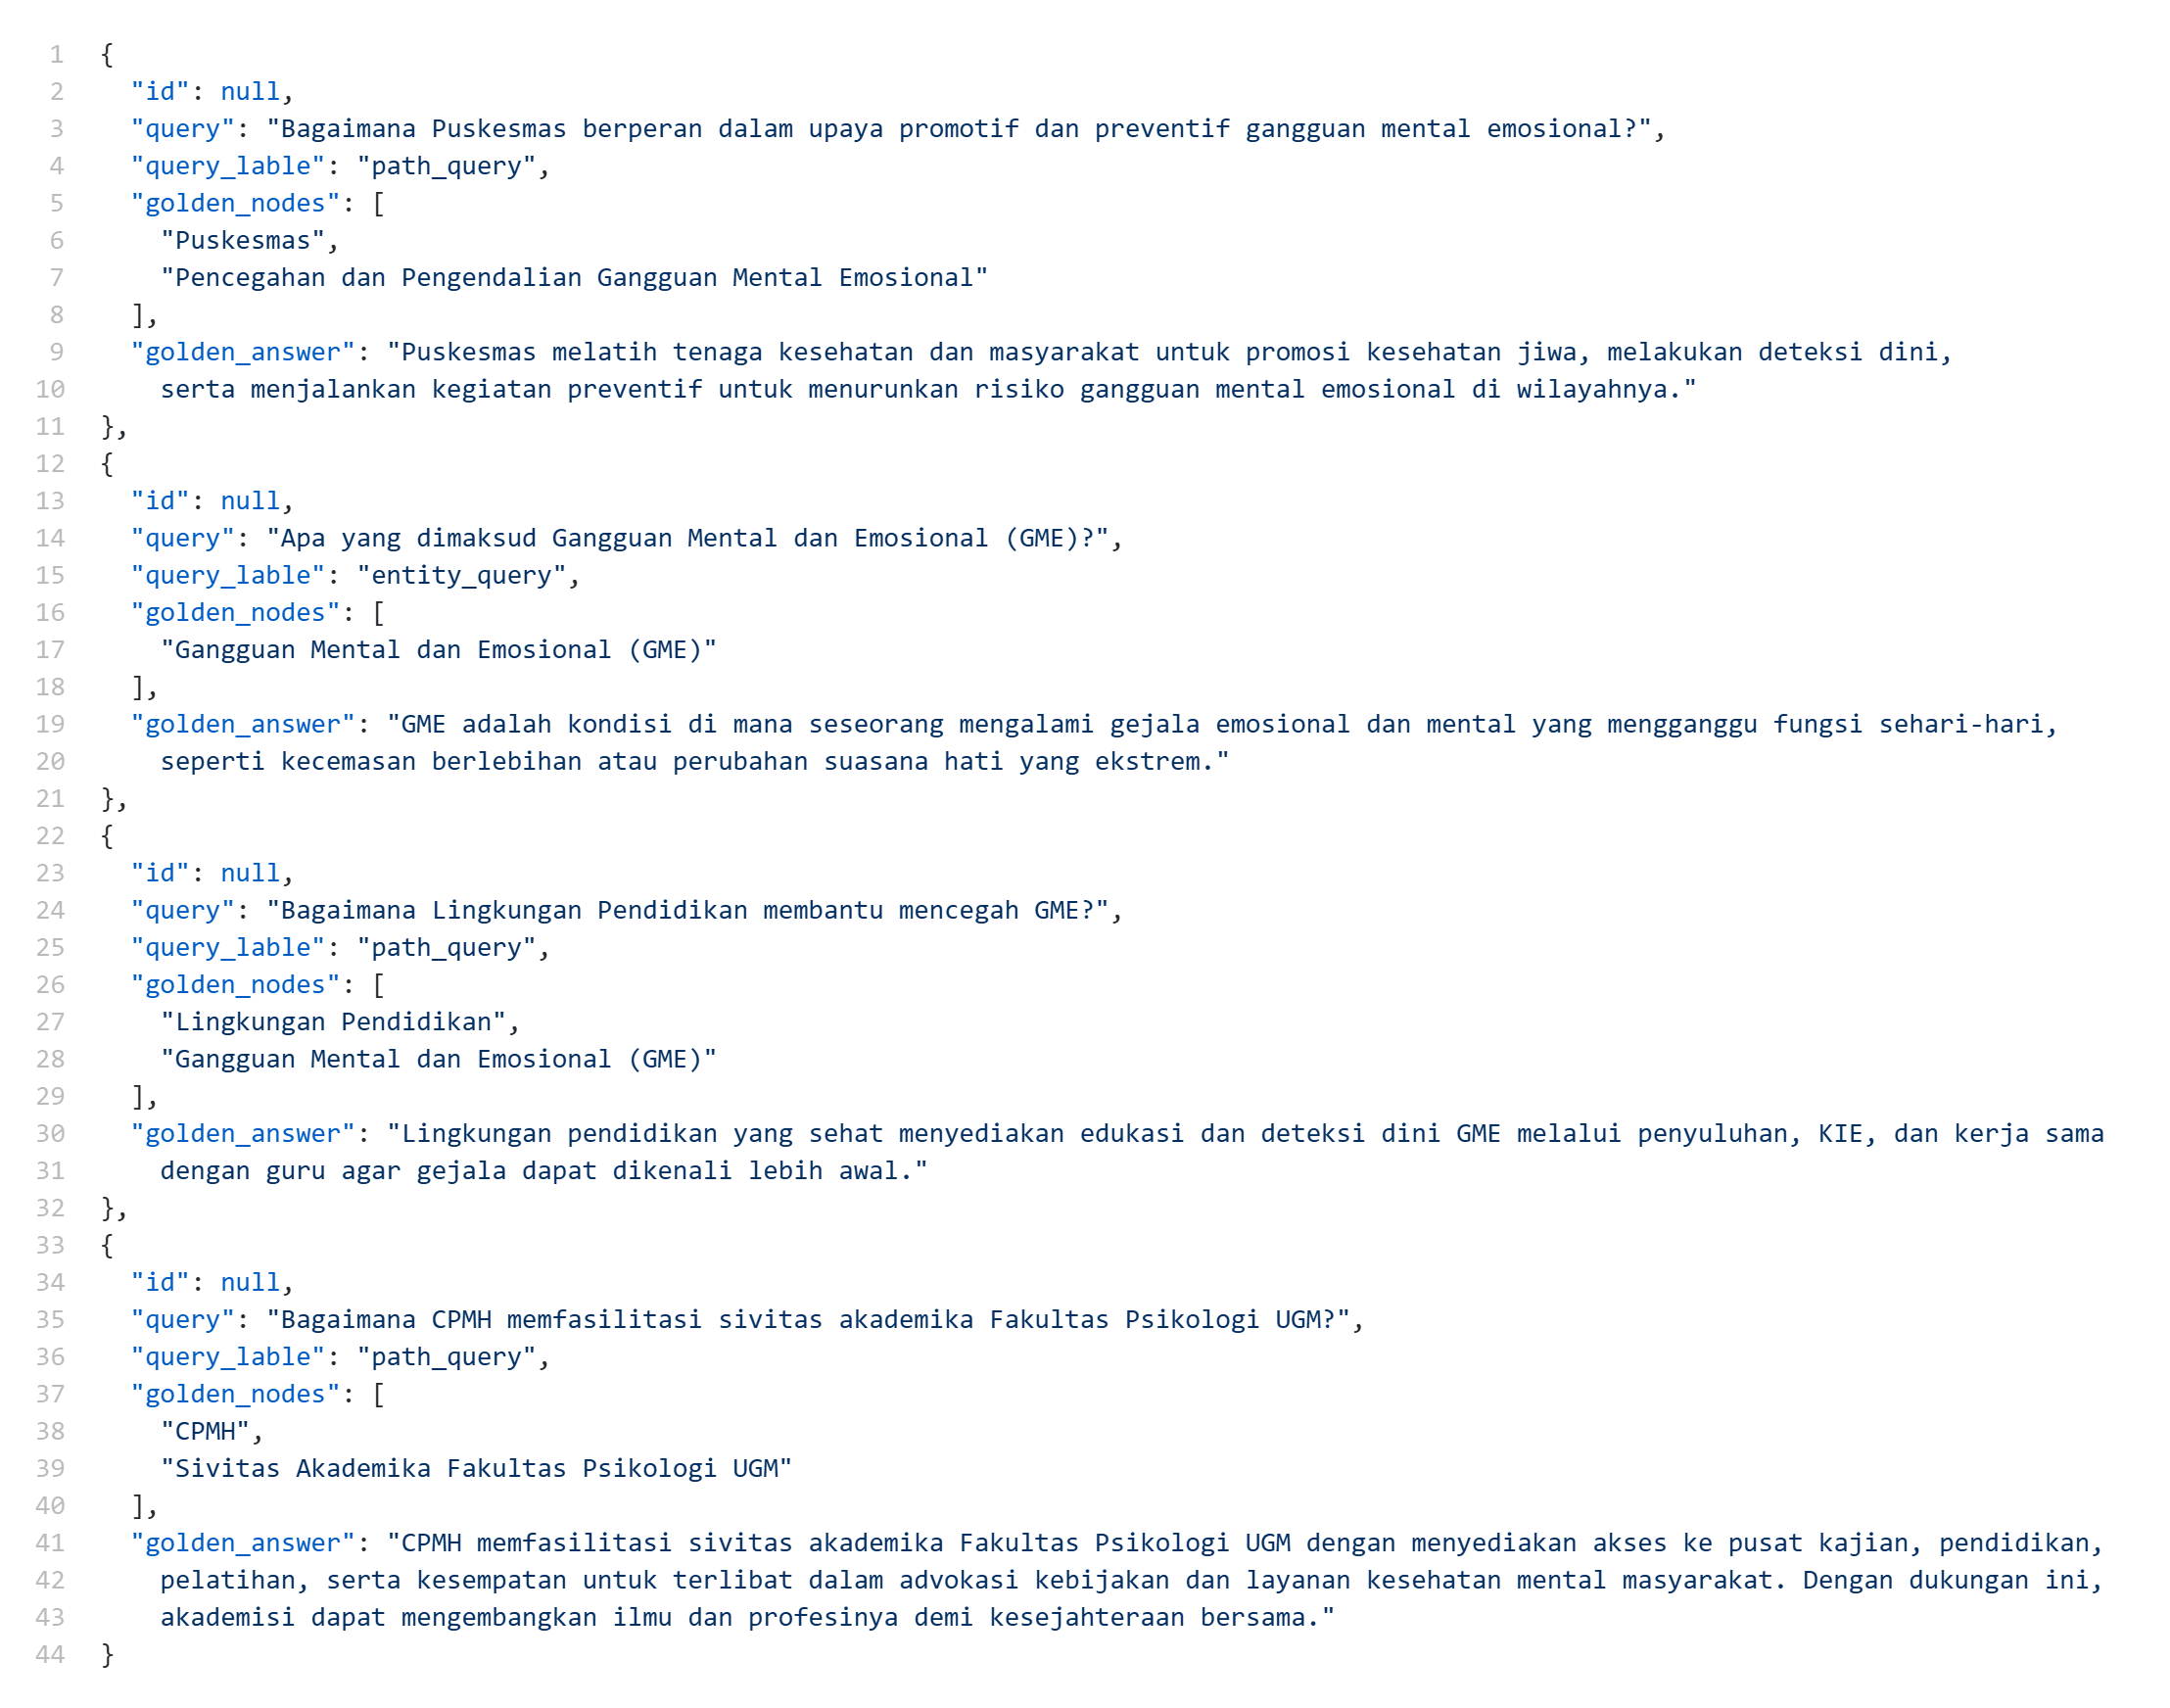
\includegraphics[width=\textwidth]{images/evaluation-dataset-example.png}}
	\caption{Contoh \textit{dataset} evaluasi sintesis yang dihasilkan oleh LLM}
	\label{fig:evaluation-dataset-example}
\end{figure}

Gambar \ref{fig:evaluation-dataset-example} menunjukkan contoh \textit{dataset} evaluasi yang mencakup kategori \\ \texttt{entity\_query} dan \texttt{path\_query}.
Setiap data sintetis terdiri dari 4 \textit{field} yaitu \textit{query}, \textit{query lable}, \textit{golden nodes}, dan \textit{golden answer}.
\textit{Query} merupakan pertanyaan yang jawabannya dapat diketahui dari informasi pada \textit{Knowledge Graph}.
Setiap kueri memiliki kategori yaitu \textit{entity query} atau \textit{path query} yang terdapat pada \textit{query lable}.
\textit{Golden nodes} berisi \textit{nodes} yang diperlukan untuk menjawab pertanyaan pada \textit{field query}, sedangkan \textit{golden answer} merupakan jawaban yang dianggap benar untuk menjawab pertanyaan.

Pertanyaan \textit{"Apa yang dimaksud Gangguan Mental Emosional (GME)?"} termasuk ke dalam \texttt{entity\_query} karena menanyakan definisi dari suatu entitas yaitu Gangguan Mental Emosional (GME).
Jawaban dari pertanyaan tersebut seharusnya dapat ditemukan pada \textit{node} Gangguan Mental Emosional (GME) atau \textit{nodes} tetangganya.
\textit{Golden nodes} yang digunakan sebagai konteks untuk menjawab pertanyaan ini adalah Gangguan Mental Emosional (GME), sesuai dengan pertanyaan yang spesifik menanyakan GME.
\textit{Golden answer} yang dihasilkan secara langsung menjawab pertanyaan sesuai konteks yang diberikan yaitu dengan memberikan definisi dari GME.

Pada pertanyaan \textit{"Bagaimana CPMH memfasilitasi sivitas akademika Fakultas Psikologi UGM?"} terlihat ada dua entitas yang terkandung, yaitu CPMH dan sivitas akademika Fakultas Psikologi.
Pertanyaan tersebut termasuk dalam \texttt{path\_query} karena jawabannya seharusnya dapat diperoleh dengan melihat hubungan antar entitas yang terkandung di dalamnya.
Untuk menjawab pertanyaan tersebut diperlukan dua \textit{nodes}, yaitu CPMH dan Sivitas Akademika Fakultas Psikologi UGM seperti yang ada pada \textit{golden nodes} beserta \textit{nodes} lain yang berada di antara keduanya.
Jawaban yang terdapat pada \textit{golden answer} menjawab pertanyaan dengan memberikan hubungan antara CPMH dan sivitas akademika Fakultas Psikologi UGM, yaitu sebagai fasilitator, dilengkapi dengan contohnya.

\section{Analisis RAG Berbasis \textit{Knowledge Graph}}
Evaluasi sistem dilakukan pada dua keluaran utama RAG berbasis \textit{Knowledge Graph} yaitu konteks yang dikeluarkan oleh komponen \textit{retrieval} dan jawaban final yang dihasilkan.
Bagian \textit{retriever} dilakukan evaluasi untuk mengukur sejauh mana sistem dapat mengambil konteks yang relevan dari \textit{Knowledge Graph}.
Jawaban final akan diukur kualitas keluaran LLM setelah diberikan konteks dari \textit{retriever}.
Selain itu, dilakukan juga analisis kesalahan untuk mengidentifikasi penyebab kegagalan sistem dalam menjawab pertanyaan.

Evaluasi dilakukan dengan konfigurasi perlakuan seperti pada Tabel \ref{tab:evaluation-treatment} dengan mengatur parameter pada \textit{body} API.
Perlakuan dilakukan dengan mengatur parameter \texttt{search\_method} dan \texttt{graph\_traversal} untuk mengatur algoritma pencarian dan penelusuran graf yang digunakan oleh \textit{retriever}.
Setiap pertanyaan pada \textit{dataset} evaluasi akan ditanyakan pada sistem dengan konfigurasi parameter menurut masing-masing perlakuan.
Naive RAG atau RAG berbasis potongan dokumen digunakan sebagai \textit{baseline} yang akan dibandingkan dengan RAG berbasis \textit{Knowledge Graph}, terutama dalam hal kemampuannya menghasilkan jawaban final.

\begin{table}[H]
	\centering
	\caption{Perlakuan yang digunakan untuk mengevaluasi RAG berbasis \textit{Knowledge Graph} dengan \textit{naive} RAG sebagai \textit{baseline}}
	\label{tab:evaluation-treatment}
	\begin{tabular}{|l|p{9cm}|}
		\hline
		\textbf{Perlakuan}            & \textbf{Keterangan}                                 \\
		\hline \hline
		\textbf{Naive RAG (Baseline)} &
		RAG dengan basis \textit{document chunk} menggunakan pencarian vektor sebagai \textit{retriever}.
		\textit{Document chunk} berukuran 1.200 karakter dengan overlap 400 karakter.
		Perlakuan ini digunakan sebagai \textit{baseline} evaluasi.                         \\
		\hline
		\textbf{Default}              &
		\textit{Search method}: auto, \textit{graph traversal}: auto.

		Sistem otomatis memilih metode pencarian terbaik.
		Awalnya mencoba \textit{full-text search}, jika tidak ditemukan hasil, baru menggunakan pencarian vektor.
		Algoritma penelusuran graf ditentukan oleh modul klasifikasi kueri secara otomatis. \\
		\hline
		\textbf{Vector Search}        &
		\textit{Search method}: vector, \textit{graph traversal}: auto.

		Menggunakan pencarian node berbasis vektor (HNSW) dengan \textit{cosine similarity}.
		Algoritma penelusuran graf ditentukan oleh modul klasifikasi kueri secara otomatis. \\
		\hline
		\textbf{Neighbor Expansion}   &
		\textit{Search method}: auto, \textit{graph traversal}: neighbor\_expansion.

		Sistem menelusuri graf dengan algoritma \textit{one-hop neighbor expansion}.
		Algoritma pencarian ditentukan secara otomatis.                                     \\
		\hline
		\textbf{N-Shortest Path}      &
		\textit{Search method}: auto, \textit{graph traversal}: n-shortest\_path.

		Sistem menelusuri graf menggunakan algoritma \textit{n-shortest path}.
		Algoritma pencarian ditentukan secara otomatis.                                     \\
		\hline
	\end{tabular}
\end{table}

Hasil dari \textit{request} pada sistem untuk setiap perlakuan pada Tabel \ref{tab:evaluation-treatment} menghasilkan data yang disimpan untuk evaluasi lebih lanjut.
Data hasil \textit{request} pada sistem yang disimpan terdiri atas \texttt{knowledge}, \texttt{llm\_answer}, \texttt{latency}, dan \texttt{graph\_entities}.
Komponen dari data tersebut yang kemudian akan dijadikan bahan evaluasi.
Latensi dari masing-masing perlakuan dapat dilihat pada Gambar \ref{fig:latency-per-treatment}

\begin{figure}[H]
	\centering
	\fbox{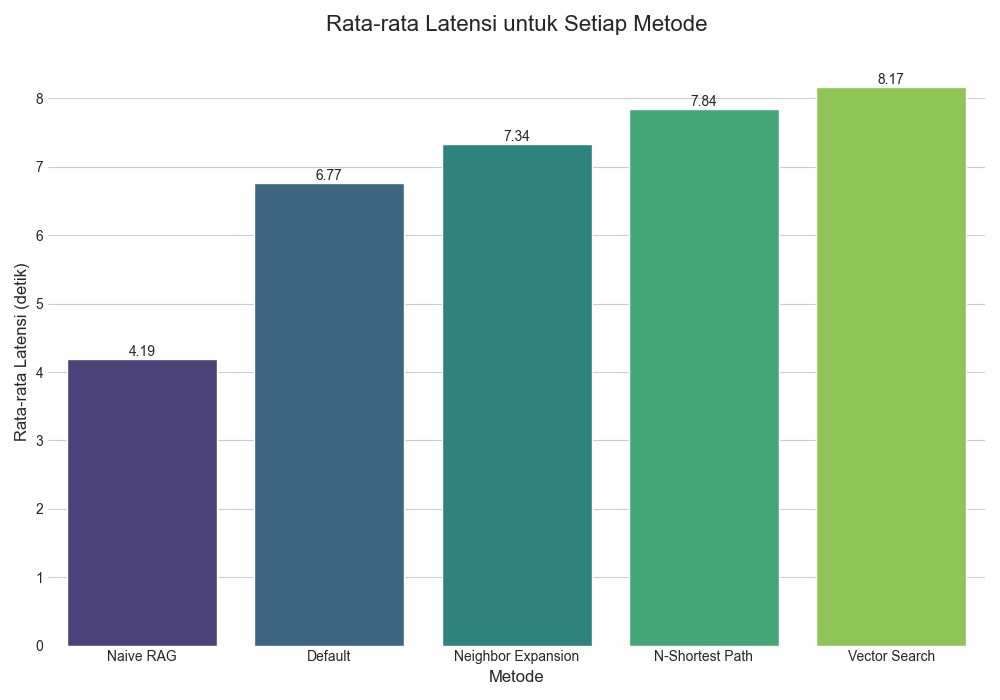
\includegraphics[width=0.8\textwidth]{images/grafik_perbandingan_latency.png}}
	\caption{Rerata latensi respons sistem pada setiap perlakuan}
	\label{fig:latency-per-treatment}
\end{figure}

Secara umum pendekatan Naive RAG memiliki rerata latensi yang lebih singkat, yaitu 4,19 detik.
Angka ini lebih unggul dari RAG-KG yang memiliki latensi lebih dari 6 detik.
Hal tersebut dapat dipahami karena pendekatan berbasis \textit{Knowledge Graph} menggunakan pemanggilan LLM melalui API setidaknya sebanyak dua kali, yaitu pada proses ekstraksi dan klasifikasi pada kueri serta pada tahap \textit{answer generation}.
Sebaliknya, Naive RAG hanya memerlukan satu kali pemanggilan LLM.
Selain itu, komponen \textit{retriever} pada Naive RAG hanya perlu mencari dan mengambil potongan-potongan dokumen berdasarkan kemiripan teks, yang merupakan operasi yang lebih cepat dan tidak memerlukan proses penelusuran kompleks.

\textit{Knowledge} atau konteks yang dihasilkan oleh komponen \textit{retriever} akan dipakai sebagai konteks tambahan bagi LLM untuk menjawab pertanyaan.
Rerata panjang konteks dari masing-masing perlakukan dapat dilihat pada Gambar \ref{fig:context-length-per-treatment}.

\begin{figure}[H]
	\centering
	\fbox{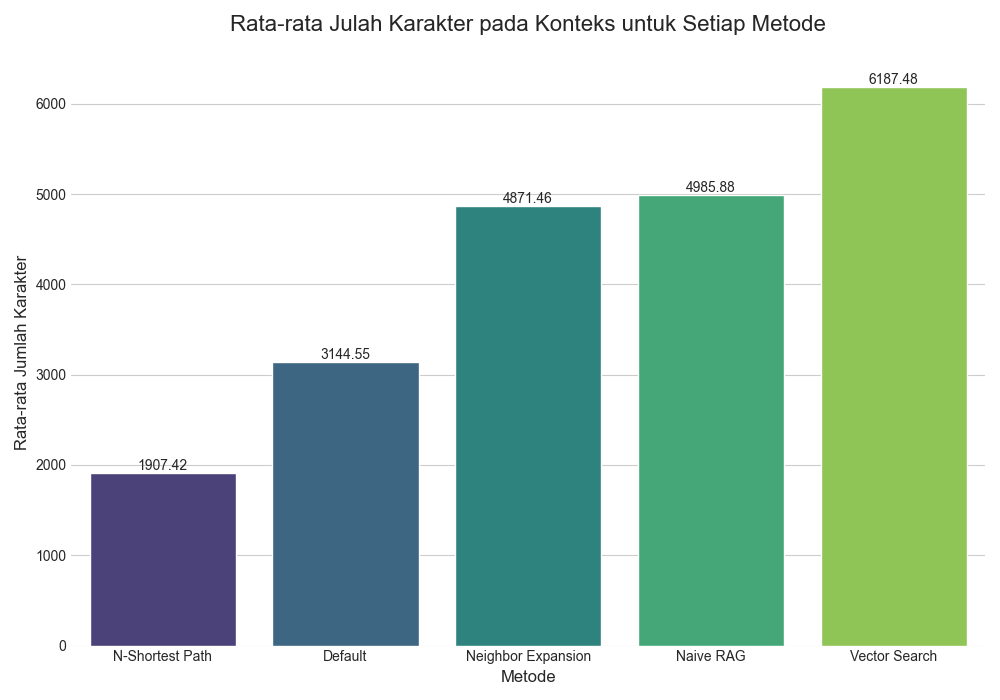
\includegraphics[width=0.8\textwidth]{images/grafik_perbandingan_konteks.png}}
	\caption{Rerata panjang konteks dari respons sistem pada setiap perlakuan}
	\label{fig:context-length-per-treatment}
\end{figure}

Dari Gambar \ref{fig:context-length-per-treatment} dapat dilihat pendekatan berbasis \textit{Knowledge Graph} secara umum memiliki panjang konteks yang lebih sedikit dari Naive RAG kecuali pada Vector Search.
Pendekatan N-Shortest Path menghasilkan rerata panjang konteks paling sedikit sebesar 1907,42 kemudian diikuti oleh Default (3144,55), Neighbor Expansion (4871,46), Naive RAG (4985,88), dan Vector Search (6187,48).
Hal tersebut dapat dipahami karena pendekatan dengan pencarian jalur menghasilkan lebih sedikit entitas dibandingkan dengan pendekatan ekspansi tetangga.
Pendekatan Default terlihat sebagai titik tengah antara N-Shortest Path dan Neighbor Expansion karena secara dinamis menentukan algoritma penelusuran graf yang sesuai.
Di sisi lain, pendekatan berbasis vektor seperti pada Naive RAG dan Vector Search cenderung menghasilkan konteks yang lebih panjang karena menggunakan $k$ dokumen atau \textit{node} teratas berdasarkan kemiripan (dengan $k=5$ dalam kasus ini), yang secara inheren cenderung menarik lebih banyak teks dibandingkan pencarian dengan \textit{full-text search}.

Konteks yang lebih panjang secara intuitif akan membuat LLM memerlukan waktu pemrosesan lebih lama yang akan memengaruhi latensi respons sistem secara keseluruhan.
Hal tersebut dapat dilihat pada Gambar \ref{fig:context-length-vs-latency} yang menunjukkan adanya hubungan positif antara panjang konteks dengan latensi sistem.
Semakin banyak konteks yang diberikan pada LLM akan menghasilkan latensi respons yang lebih lama.

\begin{figure}[H]
	\centering
	\fbox{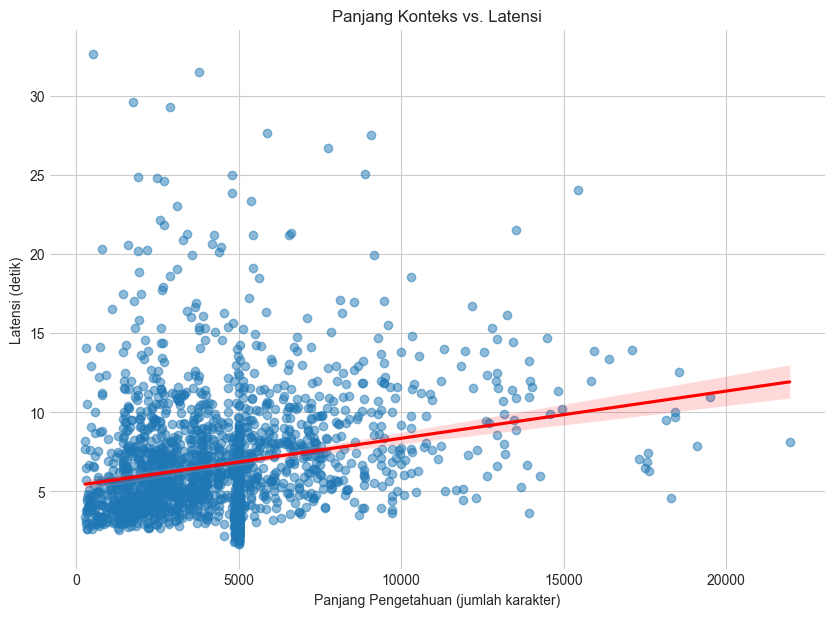
\includegraphics[width=0.8\textwidth]{images/panjag_konteks_vs_latensi.png}}
	\caption{\textit{Scatter plot} panjang konteks dengan latensi keseluruhan respons}
	\label{fig:context-length-vs-latency}
\end{figure}
\subsection{Analisis Kinerja Komponen \textit{Retriever}}

Pengujian komponen \textit{retriever} dilakukan untuk mengukur kualitas informasi atau konteks yang diambil dari \textit{Knowledge Graph}.
Informasi yang terdapat pada KG adalah kumpulan subgraf yang terdiri atas \textit{nodes} yang dihubungkan oleh \textit{edge} tertentu.
Kumpulan subgraf tersebut yang kemudian disusun dalam bentuk tekstual yang memiliki makna semantik.
Alih-alih mengevaluasi konteks yang sudah berupa teks panjang yang memerlukan alat yang dapat memahami bahasa alami seperti LLM yang kurang pasti dalam menguji, pengujian dilakukan pada \textit{nodes} yang dihasilkan sehingga evaluasi lebih terkontrol dan akurat.
Terdapat empat metrik uji untuk mengevaluasi kinerja komponen \textit{retriever}, yaitu \textit{precision}, \textit{recall}, \textit{Mean Reciprocal Rank} (MRR), dan \textit{hit ratio}.
Tabel \ref{tab:retrieval-evaluation-result} menunjukkan hasil pengujian empat metrik uji tersebut terhadap empat perlakukan RAG-KG pada Tabel \ref{tab:evaluation-treatment}.

\begin{table}[H]
	\centering
	\caption{Hasil evaluasi \textit{retriever} pada RAG berbasis \textit{Knowledge Graph} untuk masing-masing perlakuan}
	\label{tab:retrieval-evaluation-result}
	\begin{tabular}{|l|c|c|c|c|}
		\hline
		\textbf{Perlakuan}          & \textbf{Precision} & \textbf{Recall} & \textbf{MRR}    & \textbf{Hit Ratio} \\
		\hline \hline
		\textbf{Default}            & \textbf{0,1530}    & 0,8203          & \textbf{0,3758} & 0,9053             \\
		\hline
		\textbf{Vector Search}      & 0,0603             & 0,5929          & 0,1737          & 0,6744             \\
		\hline
		\textbf{Neighbor Expansion} & 0,1123             & \textbf{0,8868} & 0,3191          & \textbf{0,9584}    \\
		\hline
		\textbf{N-Shortest Path}    & 0,1245             & 0,5370          & 0,2788          & 0,6097             \\
		\hline
	\end{tabular}
\end{table}
\pagebreak

Berdasarkan hasil pada Tabel \ref{tab:retrieval-evaluation-result}, terlihat bahwa nilai rerata \textit{precision} tertinggi dicapai oleh perlakuan Default (0,1530), menunjukkan bahwa dari subgraf yang dihasilkan, metode ini memiliki relevansi paling tinggi.
Meskipun demikian, nilai presisi 0,1530 masih tergolong rendah karena hanya sekitar 15.3\% dari total \textit{node} yang diambil benar-benar relevan.
Dengan kata lain, mayoritas \textit{node}, yaitu sekitar 85\% dari konteks yang dihasilkan oleh metode ini merupakan \textit{noise}.
Metode Vector Search memiliki \textit{precision} terendah (0,0603), mengindikasikan lebih banyak informasi yang tidak relevan diambil secara proporsional.

Pada metrik \textit{Recall}, hasil yang sangat baik diperoleh oleh Neighbor Expansion (0,8868) dan Default (0,8203), yang berarti metode ini mampu mengambil hampir seluruh informasi relevan dari \textit{Knowledge Graph}.
Di sisi lain, metode N-Shortest Path dan Vector Search mencatat nilai \textit{recall} yang relatif rendah (0,5370 dan 0,5929), menandakan adanya keterbatasan dalam menjangkau konteks relevan.


Metrik \textit{Mean Reciprocal Rank} tertinggi dicapai oleh Default (0,3758) dan diikuti Neighbor Expansion (0,3191), mengindikasikan bahwa konteks yang relevan cenderung berada pada urutan atas hasil pencarian (urutan 2 hingga 3 secara rata-rata).
Sebaliknya, Vector Search (0,1737) dan N-Shortest Path (0,2788) menempati posisi bawah  yang mengindikasikan konteks relevan sering berada pada urutan bawah (urutan 5 sampai 6 secara rata-rata).
Untuk \textit{Hit Ratio}, nilai tertinggi diraih oleh Neighbor Expansion (0,9584), diikuti Default (0,9053), menandakan bahwa metode tersebut hampir selalu berhasil menemukan setidaknya satu konteks relevan dalam hasil pencarian.
Sebaliknya, N-Shortest Path dan Vector Search mencatat \textit{hit ratio} yang rendah 0,6097 dan 0,6744, menunjukkan bahwa masih ada kemungkinan yang cukup besar (30\% hingga 40\%) informasi gagal ditemukan.

Dari keempat metrik uji \textit{retriever}, terlihat perlakuan Neighbor Expansion dan Default memperoleh masing-masing dua metrik dengan nilai tertinggi dalam pengujian.
Metode Default unggul pada \textit{precision} dan MRR, sedangkan Neighbor Expansion unggul pada \textit{recall} dan \textit{hit ratio}.
Hal ini mengindikasikan bahwa Default lebih selektif dalam mengambil konteks, sedangkan Neighbor Expansion lebih agresif dan luas cakupannya, sehingga \textit{recall}-nya tinggi tetapi precision-nya moderat.
Neighbor Expansion cenderung menghasilkan data yang lebih lengkap tetapi mengandung lebih banyak noise dibandingkan dengan Default.
Hal tersebut dapat dipahami karena metode ini mengambil \textit{node} yang relevan dan \textit{nodes} tetangganya yang jumlahnya cukup banyak.
Di sisi lain, Default memilih algoritma penelusuran graf secara adaptif, sesuai dengan klasifikasi kueri, yang lebih sesuai dengan kebutuhan meskipun kalah dalam hal kelengkapan informasi.
Vector Search cenderung kurang optimal di semua metrik, menunjukkan bahwa pendekatan berbasis vektor saja kurang efektif dalam melakukan pencarian dalam graf.
Sementara itu, N-Shortest Path memberikan hasil yang kurang optimal untuk menangani sebagian besar kueri.
Secara keseluruhan, Neighbor Expansion dan Default menjadi opsi utama \textit{retriever} dalam menghadapi mayoritas pertanyaan.


\subsection{Analisis Respons Final}
Pengujian respons final dilakukan untuk mengukur kualitas jawaban akhir yang dihasilkan oleh RAG berbasis \textit{Knowledge Graph} setelah diberikan konteks tambahan oleh komponen \textit{retriever}.
Informasi berupa subgraf yang terdiri dari kumpulan \textit{nodes} dan \textit{edges} yang terhubung ditransformasikan ke dalam bentuk tekstual yang lebih bermakna secara semantik.
Bentuk tekstual tersebut kemudian dijadikan sebagai konteks untuk memberikan informasi tambahan dalam menghasilkan jawaban.
Jawaban akhir dievaluasi dengan memperhatikan empat parameter, yaitu pertanyaan, jawaban yang dihasilkan, konteks, dan jawaban seharusnya sebagai \textit{ground truth}.

Evaluasi dilakukan dengan \textit{framework} RAGAS (\textit{Retrieval-Augmented Generation Assessment}), yang merupakan evaluator RAG dengan salah satu alat ujinya menggunakan LLM.
Metrik uji untuk mengevaluasi jawaban adalah \textit{similarity}, \textit{correctness}, \textit{relevancy}, dan \textit{faithfulness} yang merupakan metrik bawaan RAGAS.
Tabel \ref{tab:final-answer-evaluation-result} menunjukkan hasil evaluasi RAGAS pada masing-masing perlakukan, termasuk dengan \textit{baseline} Naive RAG.

\begin{table}[H]
	\centering
	\caption{Hasil evaluasi jawaban final pada RAG berbasis \textit{Knowledge Graph} untuk masing-masing perlakuan dan dibandingkan dengan \textit{baseline} Naive RAG}
	\label{tab:final-answer-evaluation-result}
	\begin{tabular}{|l|c|c|c|c|}
		\hline
		\textbf{Perlakuan}          & \textbf{Similarity} & \textbf{Correctness} & \textbf{Relevancy} & \textbf{Faithfulness} \\
		\hline \hline
		\textbf{Naive RAG}          & 0,9048              & 0,3391               & 0,6996             & 0,8993                \\
		\hline
		\textbf{Default}            & 0,9242              & 0,4155               & 0,8624             & \textbf{0,9435}       \\
		\hline
		\textbf{Vector Search}      & 0,9115              & 0,3895               & 0,7387             & 0,8902                \\
		\hline
		\textbf{Neighbor Expansion} & \textbf{0,9248}     & \textbf{0,4246}      & \textbf{0,8723}    & 0,9428                \\
		\hline
		\textbf{N-Shortest Path}    & 0,9033              & 0,3936               & 0,7900             & 0,4614                \\
		\hline
	\end{tabular}
\end{table}

Metrik \textit{similarity} mengukur kesamaan semantik dengan membandingkan bentuk vektor (\textit{embedding}) antara jawaban yang dihasilkan sistem dan jawaban \textit{ground truth}.
Hasil menunjukkan bahwa semua perlakuan, termasuk \textit{baseline} Naive RAG, memiliki skor \textit{similarity} yang relatif tinggi di atas 90\%, yang menandakan bahwa sistem mampu menghasilkan jawaban yang secara umum memiliki kedekatan makna dengan jawaban seharusnya.
Nilai tertinggi dicapai oleh perlakuan Neighbor Expansion (0,9248) diikuti dengan Default (0,9242), yang mengindikasikan bahwa perluasan konteks berbasis \textit{Knowledge Graph} secara umum sama efektifnya dalam menjaga kesamaan makna dibandingkan dengan \textit{baseline}.

Metrik \textit{correctness} menilai kebenaran faktual dari jawaban yang dihasilkan.
Hasil menunjukkan peningkatan hingga sebesar 8,55\% pada perlakuan yang memanfaatkan \textit{Knowledge Graph} khususnya pada perlakuan Neighbor Expansion (0,4246) dan  Default (0,4155) dibanding \textit{baseline} Naive RAG (0,3391).
Pada metrik ini, semua metode RAG-KG menunjukkan adanya peningkatan akurasi faktual dibandingkan dengan Naive RAG.
Peningkatan ini secara langsung mengatribusikan kemampuan RAG-KG dalam menyajikan konteks faktual dari KG sebagai faktor yang berhasil meningkatkan akurasi kebenaran dari jawaban akhir.

Relevansi menunjukkan sejauh mana jawaban yang dihasilkan sistem tetap fokus dan sesuai dengan pertanyaan yang diajukan.
Neighbor Expansion (0,8723) dan Default (0,8624) menunjukkan peningkatan sebesar 17\% dari Naive RAG (0,6996) pada metrik ini.
Peningkatan tersebut menunjukkan bahwa konteks yang dihasilkan dari \textit{Knowledge Graph} tidak hanya memberikan jawaban yang lebih faktual, tetapi juga lebih tepat sasaran.
Konteks yang lebih tepat sasaran akan membuat LLM lebih mudah dalam menghasilkan jawaban yang lebih relevan dengan pertanyaan.

\textit{Faithfulness} mengukur kesesuaian informasi dalam jawaban terhadap konteks yang diberikan oleh \textit{retriever}.
Hampir semua metode menghasilkan skor di atas 0,89, kecuali pada metode N-Shortest Path yang memiliki skor sangat rendah (0,4614), menandakan bahwa metode ini lebih sering menghasilkan jawaban yang tidak konsisten atau tidak sepenuhnya didukung oleh konteks.
Nilai tinggi pada Default (0,9435) dan Neighbor Expansion (0,9428) menunjukkan bahwa strategi ini paling konsisten dalam menggunakan informasi yang tersedia.
RAG-KG dengan strategi tersebut tetap lebih tinggi sekitar 4\% dibandingkan dengan \textit{baseline} Naive RAG menghasilkan skor (0,8993).
Ini adalah bukti bahwa konteks yang diperkaya oleh \textit{Knowledge Graph} dengan pemilihan metode yang tepat secara efektif dapat mengurangi LLM dari halusinasi atau mengarang informasi.

Hasil evaluasi jawaban final secara umum menunjukkan bahwa penggunaan \textit{Knowledge Graph} yang tepat dapat meningkatkan kualitas jawaban akhir secara signifikan.
Peningkatan tertinggi dari \textit{baseline} dapat diperoleh sistem RAG-KG yang mengimplementasikan metode Default dan Neighbor Expansion hingga 8\% secara rata-rata.
Penggunaan metode Vector Search secara umum menunjukkan peningkatan dibandingkan dengan Naive RAG meskipun tertinggal dari RAG-KG dengan metode pencarian \textit{full-text} (Default dan Neighbor Expansion) dalam hal relevansi dan \textit{correctness}.
Sementara itu, penggunaan N-Shortest Path dalam melakukan penelusuran graf secara umum berpotensi menghasilkan jawaban yang tidak akurat ditandai dengan skor \textit{faithfulness} yang sangat rendah, bahkan lebih rendah dibandingkan dengan \textit{baseline}.

\subsection{Analisis Kesalahan dan Studi Kasus}

Analisis terakhir adalah meninjau secara langsung jawaban yang dihasilkan oleh masing-masing metode.
Pada studi kasus kueri \textit{"Apa yang dimaksud dengan gejala psikotik?"}, terlihat perbedaan kualitas jawaban yang dihasilkan oleh berbagai metode RAG berbasis \textit{Knowledge Graph}.
Jawaban yang diharapkan (\textit{golden answer}) memuat penjelasan singkat bahwa gejala psikotik meliputi halusinasi atau delusi seperti mendengar suara, yang dapat memengaruhi pola pikir dan berisiko terkait pikiran bunuh diri.
Hasil jawaban secara lengkap dapat dilihat pada Tabel \ref{tab:final-answer-case-1}.

\begin{longtable}{|p{2cm}|p{11cm}|}
	\caption{Komparasi kueri dan jawaban oleh masing-masing metode} \label{tab:final-answer-case-1}                                                                                                                                                                                                                                \\
	\hline
	\textbf{Kueri}                  & Apa yang dimaksud dengan gejala psikotik?                                                                                                                                                                                                                                                    \\
	\hline \hline

	\textbf{Golden Answer}          & Gejala psikotik meliputi halusinasi atau delusi seperti mendengar suara yang dapat memengaruhi cara seseorang berpikir dan berisiko terkait pikiran bunuh diri. (\textbf{Terdapat Konteks})                                                                                                  \\
	\hline
	\textbf{Naive RAG}              & Mohon maaf, konteks yang diberikan tidak menjelaskan apa yang dimaksud dengan gejala psikotik. Konteks tersebut hanya menyebutkan tentang individu risiko tinggi psikotik dan pencegahan transisi menjadi gangguan psikotik. (\textbf{Terdapat Konteks})                                     \\
	\hline
	\textbf{Default}                & Gejala psikotik adalah gejala yang mungkin dialami oleh Orang dengan Kebutuhan Disabilitas (OKBD) yang bisa memengaruhi keinginan bunuh diri, contohnya adalah mendengar suara-suara. (\textbf{Terdapat Konteks})                                                                            \\
	\hline
	\textbf{Vector \newline Search} & Saya mohon maaf, saya tidak menemukan informasi spesifik mengenai "gejala psikotik" dalam pengetahuan yang saya miliki. Pengetahuan yang tersedia lebih berfokus pada keluhan fisik, gejala somatik, faktor biologis, dan tanda bahaya kecenderungan bunuh diri. (\textbf{Terdapat Konteks}) \\
	\hline
	\textbf{Neighbor Expansion}     & Gejala psikotik adalah gejala yang mungkin dialami oleh Orang dengan Kondisi Biologis dan Diagnosa (OKBD) yang bisa memengaruhi keinginan bunuh diri, seperti mendengar suara-suara. Gejala ini juga dapat memperbesar risiko bunuh diri. (\textbf{Terdapat Konteks})                        \\
	\hline
	\textbf{N-Shortest Path}        &
	\begin{minipage}[t]{10cm}
		Gejala psikotik adalah serangkaian pengalaman yang menunjukkan hilangnya kontak dengan realitas. Ini sering kali melibatkan perubahan dalam pikiran, persepsi, dan perilaku seseorang.

		Gejala psikotik utama meliputi:
		\begin{enumerate}
			\item \textbf{Halusinasi:} Persepsi sensorik tanpa rangsangan eksternal.
			\item \textbf{Delusi:} Keyakinan salah yang bertahan meskipun ada bukti bertentangan.
			\item \textbf{Pemikiran dan Bicara Tidak Terorganisir:} Kesulitan mengatur pikiran sehingga bicara menjadi kacau.
			\item \textbf{Perilaku Tidak Terorganisir atau Katatonik:} Perilaku aneh, agitasi, atau tidak bergerak sama sekali.
		\end{enumerate}
		(\textbf{Tanpa Konteks})
		\vspace{0.5em}
	\end{minipage}                                                                                                                                          \\
	\hline
\end{longtable}

Metode Naive RAG gagal memberikan jawaban yang diharapkan, yaitu definisi gejala psikotik, hanya menyampaikan bahwa konteks tidak menjelaskan gejala psikotik dan sekadar menyinggung individu berisiko tinggi psikotik serta pencegahan transisi menjadi gangguan psikotik.
Jawaban tersebut menunjukkan bahwa \textit{retriever} gagal dalam memberikan konteks yang relevan dan sesuai untuk menjawab pertanyaan.
Hal serupa juga dapat dilihat pada metode Vector Search, yang menunjukkan jawaban yang mengaku tidak menemukan informasi spesifik dan malah memaparkan topik terkait keluhan fisik, faktor biologis, dan tanda bahaya kecenderungan bunuh diri, yang kurang relevan dengan pertanyaan.
Hal ini membuktikan bahwa untuk kueri yang menuntut definisi istilah khusus, pencarian semantik berbasis vektor masih memiliki potensi kegagalan dalam mengambil konteks.


Sebaliknya, Default dan Neighbor Expansion berhasil mendekati topik yang benar, menyebutkan bahwa gejala psikotik dapat memengaruhi keinginan bunuh diri dan memberikan contoh seperti mendengar suara-suara.
Munculnya istilah "OKBD" yang tidak sepenuhnya relevan dapat dilihat sebagai efek samping dari penelusuran graf, di mana sistem mengambil node tetangga yang terhubung namun berada di luar konteks jawaban yang ideal.
Meskipun demikian, hal ini menunjukkan pendekatan yang jauh lebih efektif daripada pencarian berbasis vektor seperti pada Naive RAG dan Vector Search.

Di sisi lain metode N-Shortest Path menghasilkan jawaban yang secara definisi umum sangat lengkap dan mencakup empat gejala utama (halusinasi, delusi, pemikiran/bicara tidak terorganisir, dan perilaku tidak terorganisir atau katatonik).
Meskipun tampak informatif, jawaban ini merupakan bentuk halusinasi karena tidak bersumber dari konteks yang diambil oleh \textit{retriever}.
\textit{Retriever} gagal untuk mengambil konteks dari \textit{Knowledge Graph} yang menyebabkan LLM memanfaatkan pengetahuan internalnya untuk mengisi kekosongan informasi.
Kegagalan tersebut dapat dipicu oleh algoritma \textit{shortest path} di mana tidak ditemukannya jalur di antara \textit{nodes} yang terdeteksi.
Hal tersebut dapat terjadi apabila memaksakan pertanyaan yang termasuk ke dalam \textit{entity query} dalam kasus ini \textit{"Apa yang dimaksud dengan gejala psikotik?"} yang menanyakan definisi akan suatu hal.

Dari kasus ini dapat disimpulkan bahwa kelengkapan jawaban tidak selalu berarti kualitas RAG yang baik.
Metode yang terlihat "pintar" seperti N-Shortest Path memiliki kemungkinan untuk berhalusinasi jika gagal mengambil konteks yang relevan.
Di sisi lain, metode Default dan Neighbor Expansion berhasil mengambil konteks relevan sehingga mampu memanfaatkannya untuk menghasilkan jawaban yang akurat dan terpercaya.
Kedua metode tersebut menunjukkan kejujuran sistem, berlandaskan konteks, dan cenderung lebih \textit{faithful} dan dapat dipercaya.

% Berikut ini adalah yang perlu diperhatikan untuk mengisi bab hasil dan pembahasan:

% \begin{enumerate}
% 	\item Setiap rumusan masalah boleh memiliki lebih dari 1 tujuan.
% 	\item Setiap subbab harus spesifik menjawab setiap tujuan yang dituliskan.
% 	\item Setiap rumusan masalah boleh dijawab dengan 1 subbab atau lebih.
% \end{enumerate}

% Berikut ini adalah contoh sub bab untuk menjelaskan tujuan penelitian.

% \section{Pembahasan Tujuan 1 dengan Hasil Penelitian 1 (Ubah Judul Sesuai dengan Hal yang Hendak dibahas)}

% Sub bab pertama adalah membahas tujuan penelitian pertama dengan hasil penelitian ke-1.
% Dapat ditambahkan beberapa sub bab jika diperlukan.

% \section{Pembahasan Tujuan 1 dengan Hasil Penelitian 2 (Ubah Judul Sesuai dengan Hal yang Hendak dibahas)}

% Sub bab kedua adalah membahas tujuan penelitian pertama dengan hasil penelitian ke-2. Sub bab ini merupakan contoh tambahan sub bab pertama.

% \section{Pembahasan Tujuan 2 dengan Hasil Penelitian 3 (Ubah Judul Sesuai dengan Hal yang Hendak dibahas)}

% Sub bab ketiga adalah membahas tujuan penelitian kedua. Dapat ditambahkan beberapa sub bab jika diperlukan.

% \section{Perbandingan Hasil Penelitian dengan Hasil Terdahulu}

% Pembahasan penutup dapat menjelaskan mengenai kelebihan hasil pengembangan /
% penelitian dan kekurangan dibandingkan dengan skripsi atau penelitian terdahulu atau
% perbandingan terhadap produk lain yang ada di pasaran. Penulis dapat menggunakan tabel untuk membandingkan secara gamblang dan menjelaskannya.
\cleardoublepage \phantomsection
\chapter{Kesimpulan dan Saran}
\section{Kesimpulan}
Berdasarkan penelitian yang telah dilakukan, metode RAG berbasis \textit{Knowledge Graph} secara umum mengungguli Naive RAG yang berbasis potongan dokumen pada mayoritas metrik uji.
Hasil evaluasi terhadap beberapa metode pengambilan konteks dari \textit{Knowledge Graph} serta analisis kualitas jawaban akhir menghasilkan beberapa kesimpulan utama sebagai berikut:

\begin{enumerate}
      \item Arsitektur RAG Berbasis \textit{Knowledge Graph} terbukti mampu meningkatkan akurasi dan konsistensi respons.
            Penelitian ini berhasil merancang dan mengimplementasikan arsitektur \textit{chatbot} yang mengintegrasikan RAG dengan KG.
            Hasil evaluasi menunjukkan bahwa arsitektur ini secara konsisten mengungguli pendekatan Naive RAG, yang dibuktikan dengan peningkatan \textlatin{correctness} sebesar 8\%, \textit{relevancy} sebesar 17\%, dan \textit{faithfulness} sebesar 4\%.
            Peningkatan ini menegaskan bahwa integrasi struktur graf mampu menghasilkan respons yang lebih akurat secara faktual, relevan, dan konsisten dengan basis pengetahuannya, sehingga meminimalkan masalah fundamental terkait risiko misinformasi.

      \item Metode \textit{Knowledge Extraction} yang dirancang berhasil mengonstruksi sebuah \textit{Knowledge Graph} yang koheren dan kaya, terdiri dari 1.119 entitas unik dan 1.078 relasi yang diekstraksi dari korpus literatur.
            Efektivitas proses KE dalam memetakan hubungan kompleks dari literatur tervalidasi secara fungsional, yang dibuktikan oleh nilai \textit{recall} (0,8868) dan \textit{hit ratio} (0,9584) yang tinggi pada proses retrieval.
            Hal ini secara tidak langsung mengindikasikan bahwa struktur relasi yang diekstraksi cukup logis dan terorganisir dengan baik untuk memungkinkan penelusuran informasi yang mendalam dan menyeluruh.

      \item Metode \textit{retrieval} Default dan \textit{Neighbor Expansion} menunjukkan performa paling konsisten dan unggul di antara seluruh strategi RAG-KG yang diuji.
            Keduanya terbukti mampu menemukan informasi relevan dari \textit{Knowledge Graph} dan menghasilkan kualitas jawaban yang relatif lebih baik.
            Oleh karena itu, penelitian ini merekomendasikan kedua pendekatan tersebut sebagai pilihan utama untuk \textit{Knowledge Retrieval} dalam arsitektur RAG berbasis KG.
\end{enumerate}

Secara keseluruhan, penelitian ini menegaskan bahwa penggunaan \textit{Knowledge Graph} sebagai fondasi pengetahuan dalam RAG dapat meningkatkan relevansi, akurasi, dan faktualitas respons \textit{chatbot}.
Dengan memanfaatkan sumber data berupa buku dan artikel terkait kesehatan mental, sistem yang dikembangkan mampu menyajikan jawaban yang lebih informatif dan faktual, sehingga berpotensi meminimalkan risiko halusinasi saat berinteraksi dengan pengguna.

\section{Saran}
Berdasarkan penelitian yang telah dilakukan, berikut adalah beberapa saran untuk penelitian dan pengembangan selanjutnya:

\begin{enumerate}
      \item Pada penelitian ini \textit{dataset} evaluasi masih diperoleh berupa data sintetis hasil \textit{prompting} menggunakan LLM.
            Penelitian selanjutnya disarankan menggunakan \textit{dataset} pertanyaan dan jawaban yang telah divalidasi oleh ahli atau bersumber langsung dari sumber terpercaya agar evaluasi mencerminkan performa saat digunakan dalam kasus yang sebenarnya.

      \item Perlu dilakukan eksplorasi lebih lanjut terhadap \textit{tuning} parameter, seperti nilai top-k dan \textit{max hop} pada proses \textit{retrieval}, untuk menemukan konfigurasi optimal yang dapat menyeimbangkan antara kelengkapan dan relevansi konteks yang diambil.

      \item Meskipun berkinerja kurang baik, konsep pencarian jalur seperti pada \textit{N-Shortest Path} tetap memiliki potensi.
            Penelitian lebih lanjut dapat difokuskan pada penerapan mekanisme penyaringan atau pembobotan untuk memastikan hanya jalur yang paling relevan secara semantik dan kontekstual yang dipertimbangkan, sehingga dapat mengurangi risiko halusinasi.

\end{enumerate}

%======================================

%======================================
%  References
%======================================
\cleardoublepage \phantomsection
\thereferences
% You can change 
%    the filename and location of the files inputted
\bibliography{references}


%======================================

%======================================
%  Appendix
%======================================
% You can change 
%    the filename and location of the files inputted
%    use \chapterappendix for the first page of the appendix
%    use \chapterappendixadd for the next page

\appendix
\appendixtables
\appendixfigures

\cleardoublepage \phantomsection
\chapterappendix{contents/appendix/appendix-latex}
% \chapterappendixadd{contents/appendix/appendix-latex}
% \chapterappendixadd{contents/appendix/appendix-penulisan-referensi}
% \chapterappendixadd{contents/appendix/appendix-code}




%======================================

\end{document}